\section*{Appendix}
\renewcommand{\baselinestretch}{0.75}\normalsize
\tableofcontents

\section{Ethics Statement \& Reproducibility}\label{appendix:impact}
In recent years, there has been a trend in RL towards large-scale multi-task models that leverage offline pre-training.  
In this work, we broadly aim at building agents that can learn new tasks via ICL without the need for re-training or fine-tuning.
Our goal is to reduce the need to provide entire past episodes in the agent's context by augmenting the agent with an external memory in combination with a retrieval component, similar to RAG in LLMs. 
We believe that multi-task agents of the near future will be able to perform a broad range of tasks, and that these agents will greatly benefit from RAG as used in RA-DT. 
The external memory component can enable agents to leverage information from their own distant past or experiences from other agents. 
Such agents could have an immense impact on the future of work (e.g., as a source of inexpensive labour).  
As such, they do not come without risks and the potential for misuse.  
While we believe that our work can significantly impact the positive use of future agents, it is essential to ensure the responsible deployment of future technologies.

We open-source the codebase used for our experiments and release the datasets we generated \footnote{GitHub: \url{https://github.com/ml-jku/RA-DT}}. 
In addition, we provide further information on the environments/datasets, implementation including hyperparameter tables, and on our experiments in Appendices \ref{appendix:env-data}, \ref{appendix:expdetails}, \ref{appendix:results}, respectively. 



\section{Environments \& Datasets}\label{appendix:env-data}
\subsection{Dark-Room and Dark Key-Door} \label{appendix:env-data-dark}
The Dark-Room environment is modelled after Morris-Watermaze, a classic experiment in behavioural neuroscience for studying spatial memory and learning in animals \citep{Hooge:01}.
We design our Dark-Room and Dark Key-Door environments in Minihack \citep{Samvelyan:2021}, which is based on the NetHack Learning Environment \citep{kuttler2020nethack}.
We construct grids of dimensions $10\times 10$, $20\times20$, and $40\times20$, as depicted in Figure \ref{fig:minigrids}.
With increasing grid sizes, the task of locating the goal becomes harder as the number of possible positions in the grid grows (100, 400, 800).
Therefore, we set the number of interaction steps per environment equal to the number of grid cells. 
Consequently, larger grids result in longer episodes and thus context lengths (e.g., 2400 for AD).
The agent observes its own x-y position on the grid and can perform one of 5 actions at every interaction step (up, down, left, right, stay). 
Episodes start in the top left corner (0,0), and the agent is reset to the start position after every episode.

In \textbf{Dark-Room}, the agent has to navigate to a randomly placed and invisible goal position. 
Therefore, the task space in Dark-Room environments is equal to the number of grid-cells (i.e., $100$ for $10\times10$). 
The agent receives a reward of +1 for every step in the episode if it is located in the goal position and 0 otherwise. 
As there are as many grid-cells as episode steps, the optimal strategy for solving the Dark-Room task is to use the first episode to visit every cell to find the hidden goal location. 
Once found, this knowledge can be exploited in upcoming trials. 

In contrast, in \textbf{Dark Key-Door}, there are two objects: a key and a goal state. 
Similar to Dark-Room, the key and goal positions are randomly placed on the grid. 
The agent has to first pick up the invisible key and then find the invisible goal. 
Due to the presence of the two key events (picking up the key, finding the goal), the task space is combinatorial in the number of grid-cells (i.e., $100^2=10000$ for $10\times10$).
This makes the Dark Key-Door more challenging than the Dark-Room task, especially as the grid size becomes larger.

\begin{figure*}[h]
    \centering    
    \subfigure[Dark-Room 10$\times$10]{
        
\includegraphics[width=0.31\linewidth]{figures/data/darkroom10x10.png}
    }
    \hfill
    \subfigure[Dark-Room 20$\times$20]{
        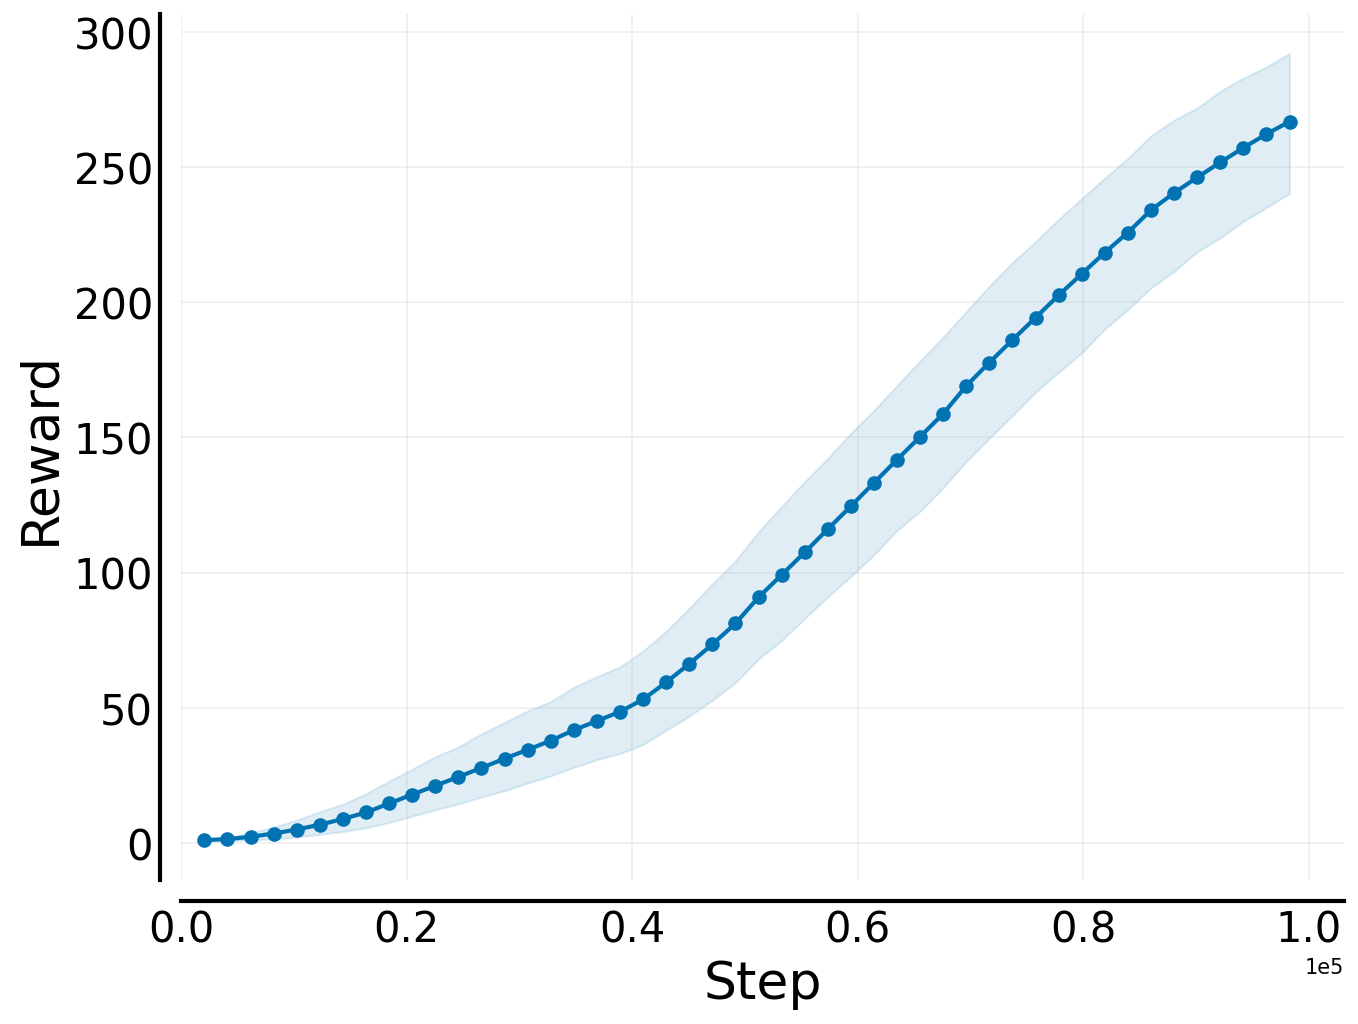
\includegraphics[width=0.31\linewidth]{figures/data/darkroom20x20.png}
    }
    \hfill
    \subfigure[Dark-Room 40$\times$20]{
        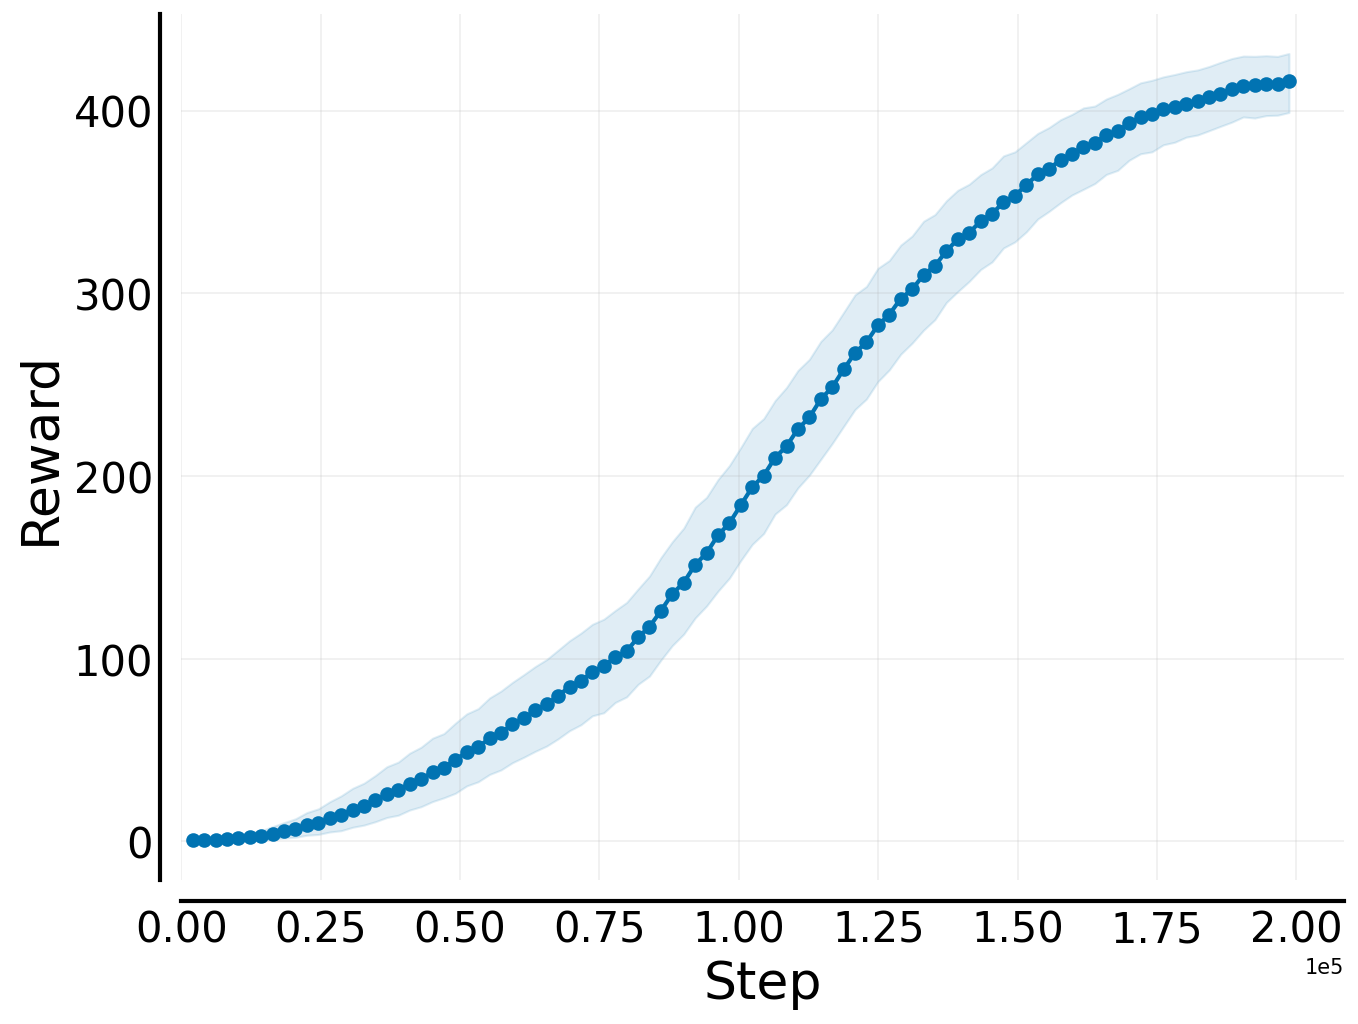
\includegraphics[width=0.31\linewidth]{figures/data/darkroom40x20.png}
    }
    \caption{Average performances of the \textbf{source algorithm}, PPO, on 80 train tasks for Dark-Room \textbf{(a)} 10$\times$10, \textbf{(b)} 20$\times$20, and \textbf{(c)} 40$\times$20.
    For (a), (b), we train PPO on individual tasks for 100K environment steps.
    For (c), we train for 200K environment steps to take the longer episode lengths into account. We evaluate the agents after every 10K steps. 
    Curves show the mean reward achieved (+ 95\% CI) across the 80 train tasks.}    
    \label{fig:datasets-source-darkroom}
\end{figure*}
\textbf{Training Dataset.}
For both Dark-Room and Dark Key-Door, we generate training datasets for 80 randomly assigned goals or key-goal combinations. 
We use PPO \citep{Schulman:2017} to generate 100K environment transitions per goal location for $10\times10$ and $20\times20$ grids and 200K environment transitions for the largest grid.
Therefore, the total number of transitions across datasets is 8M for $10\times10$ and $20\times20$ grids and 16M for $40\times20$.

We train PPO with standard hyperparameter settings in \texttt{stable-baselines3} \citep{Raffin:21} using a learning rate of $3e^{-4}$, batch size of $64$, number of steps between updates of $2048$, number of update epochs $10$, and entropy coefficient of $0.01$. 
For $20\times20$ and $40 \times 20$ grids, we increase the number of update epochs to $30$ and the entropy coefficient to $0.1$ for $40 \times 20$. We store all generated transitions of PPO for our datasets. Consequently, the final datasets contain a mixture of suboptimal or exploratory and optimal or exploitative behaviour.  

\textbf{Source Algorithm Performance.} We show average learning curves across all task-specific PPO agents on the 80 training tasks for all grid-sizes in Figures \ref{fig:datasets-source-darkroom} and \ref{fig:datasets-source-dark-keydoor} for Dark-Room and Dark Key-Door, respectively.
For the $10\times10$ grids, the average performance converges towards optimal performance. 
However, on the larger grid sizes, the performance remains below the optimum.
This is because it takes the agent longer to discover and collect successful episodes by initially random environment interaction as the grids become larger.

    
    
\begin{figure*}[h]
    \centering    
    \subfigure[Dark Key-Door 10$\times$10]{
        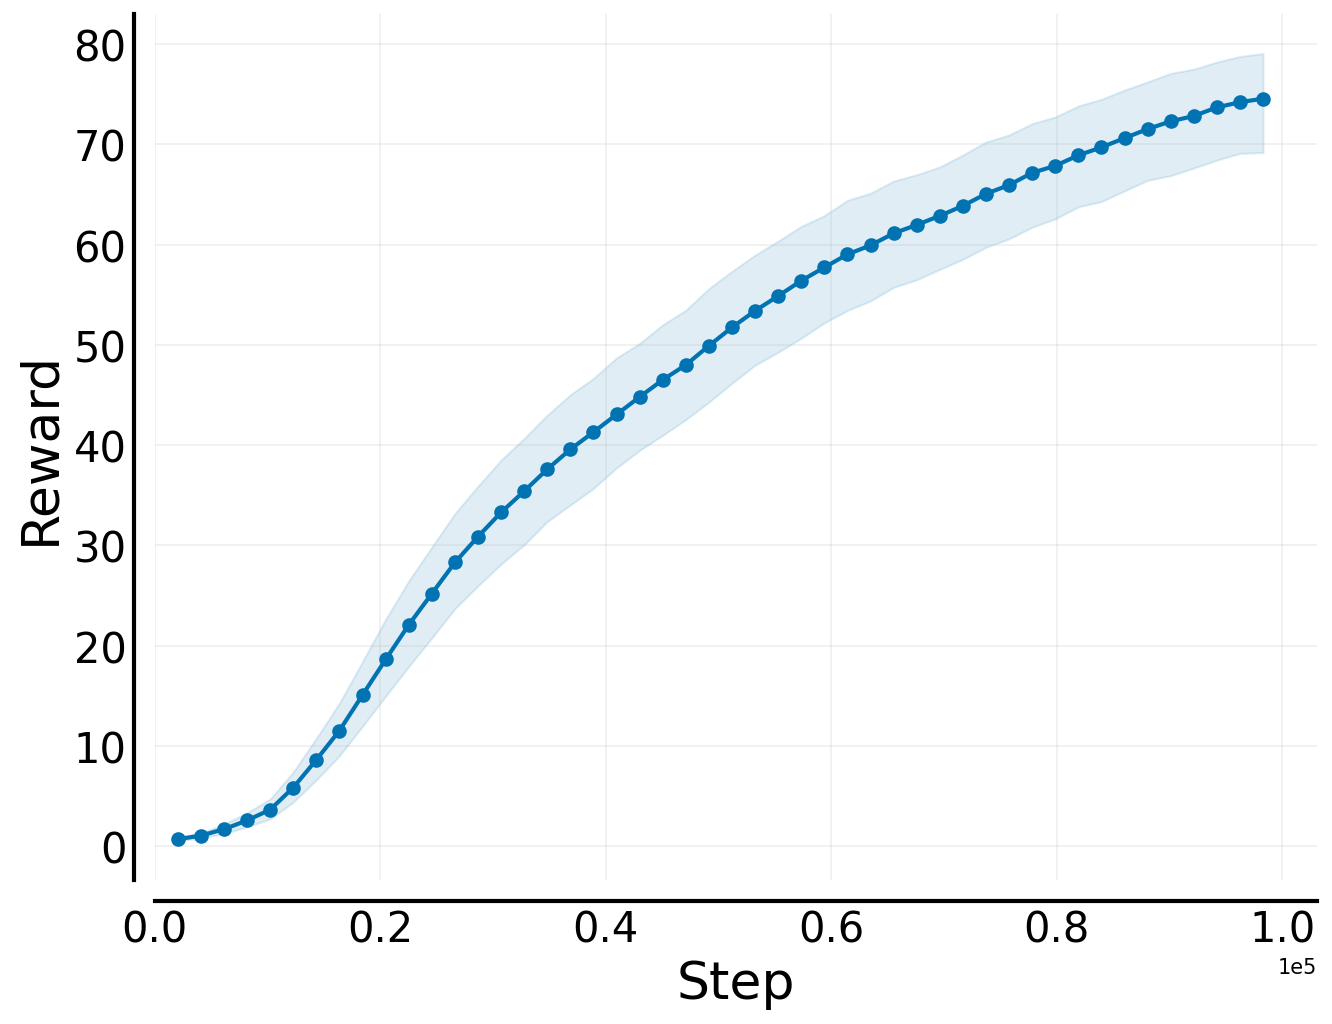
\includegraphics[width=0.31\linewidth]{figures/data/keydoor.png}
    }
    \hfill
    \subfigure[Dark Key-Door  20$\times$20]{
        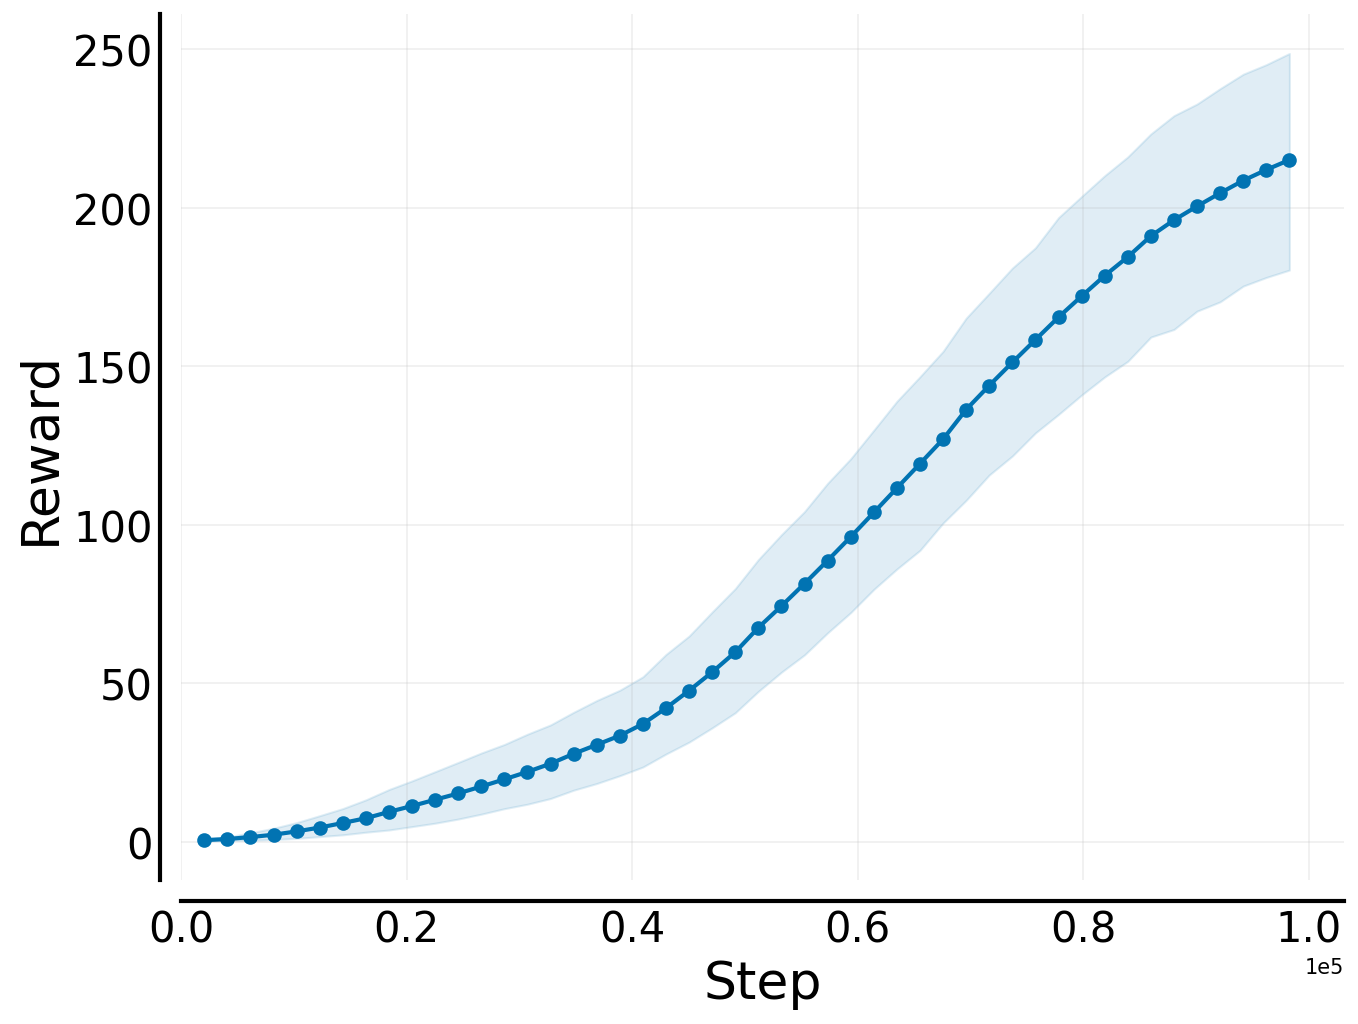
\includegraphics[width=0.31\linewidth]{figures/data/keydoor20x20.png}
    }
    \hfill
    \subfigure[Dark Key-Door  40$\times$20]{
        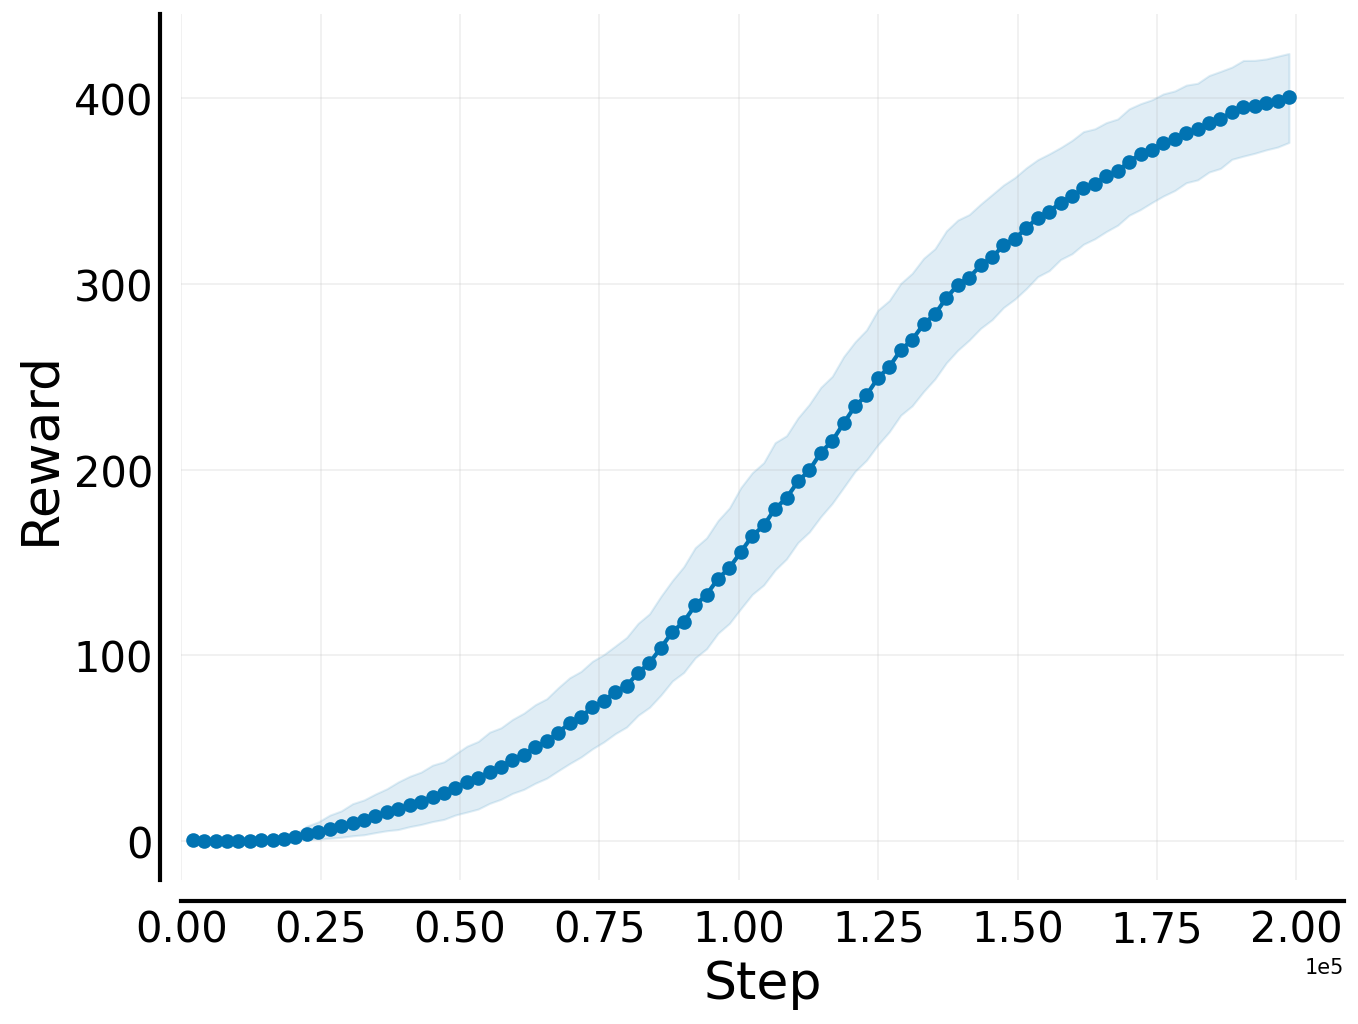
\includegraphics[width=0.31\linewidth]{figures/data/keydoor40x20.png}
    }
    \caption{Average performances of the \textbf{source algorithm}, PPO, on 80 train tasks for \textbf{Dark Key-Door}  \textbf{(a)} 10$\times$10, \textbf{(b)}  20$\times$20, and \textbf{(c)} 40$\times$20.
    For (a), (b) we train PPO on individual tasks for 100K environment steps.
    For (c), we train for 200K environment steps. We evaluate the agents after every 10K steps. 
    Curves show the mean reward achieved (+ 95\% CI) across the 80 train tasks.}    
    \label{fig:datasets-source-dark-keydoor}
\end{figure*}


\begin{figure*}[h]
    \centering
    \subfigure[Room 10$\times$10]{
        
\includegraphics[width=0.15\linewidth]{figures/envs/darkroom10x10.png}
        \label{fig:sub1}
    }
    \hspace{1cm}
    \subfigure[Key-Door 10$\times$10]{
        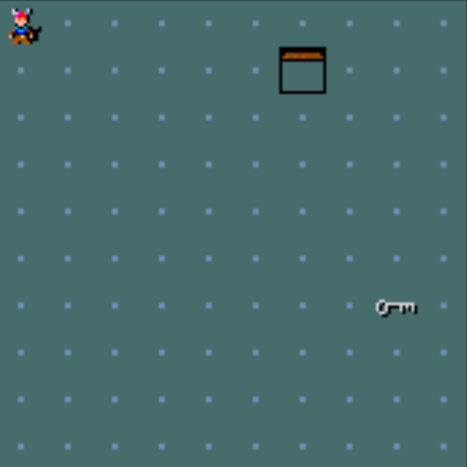
\includegraphics[width=0.15\linewidth]{figures/envs/keydoor10x10.png}
        \label{fig:sub2}
    }
    
    \subfigure[Room 20$\times$20]{
        
\includegraphics[width=0.15\linewidth]{figures/envs/darkroom20x20.png}
        \label{fig:sub1}
    }

    \subfigure[Room 40$\times$20]{
        
\includegraphics[width=0.5\linewidth]{figures/envs/darkroom40x20.png}
        \label{fig:sub1}
    }
    \caption{Mini-grid environments. In \textbf{Dark-Room}, the agent is located in a room and has to navigate to an invisible goal location. We use grid-sizes  \textbf{(a)} 10$\times$10, \textbf{(b)} 20$\times$20 and \textbf{(c)} 40$\times$20 for our experiments. In \textbf{(b) Dark-KeyDoor}, the agent has to pick up an invisible key, then navigate to the invisible goal location. Agents only observe their current x-y coordinate on the grid. A reward of +1 is obtained in every step the agent is situated in the goal state, +1 for picking up the key.}
    \label{fig:minigrids}
\end{figure*}
\clearpage
\subsection{MazeRunner}\label{appendix:env-data-mazerunner}
MazeRunner was introduced by \citep{Grigsby:23} and inspired by the Memory Maze environment \citep{Pasukonis:22}.
The agent is located in a 15$\times$15 procedurally-generated maze and has to navigate to a sequence of one, two, or three goal locations in the right order (see Figure \ref{fig:mazerunner-env}).
Similar to Dark-Room environments, MazeRunner is partially observable and exhibits sparse rewards.
The agent observes a Lidar-like 6-dimensional representation of the state that contains 4 continuous values that measure the distance from the agent's location to the nearest wall, and the x-y coordinates of the agent's position in the grid.
The action space is 4-dimensional (up, down, left, right).
A reward of +1 is obtained when reaching the currently active goal state in the goal sequence. 
Therefore, the total achievable reward is equal to the number of goal states. 
Episodes last for a maximum of 400 steps or terminate early if all goal locations have been reached. 
After every episode, the agent (gray box in Figure \ref{fig:mazerunner-env}) is reset to the origin location. 
During evaluation, we allow for 30 ICL trials, which amounts to 12K environment steps in total.
\begin{figure}[h]
    \centering
    \subfigure[One goal]{
        
\includegraphics[width=0.25\linewidth]{figures/envs/mazerunner3.png}
        \label{fig:X}
    }
    \hspace{0.5cm}
    \subfigure[Two goals]{
        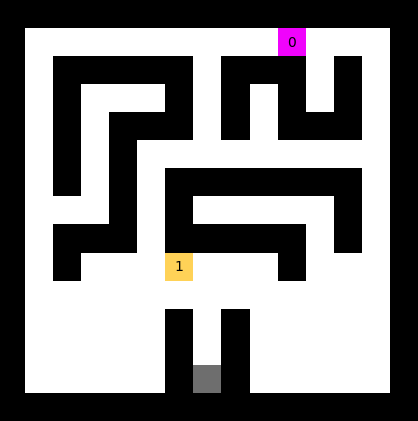
\includegraphics[width=0.25\linewidth]{figures/envs/mazerunner4.png}
        \label{fig:X}
    }
    \hspace{0.5cm}
    \subfigure[Three goals]{
        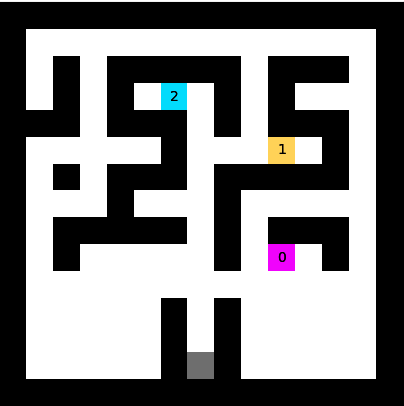
\includegraphics[width=0.25\linewidth]{figures/envs/mazerunner1.png}
        \label{fig:X}
    }
    \caption{Maze-Runner environments introduced by \citet{Grigsby:23}. In \textbf{Maze-Runner}, the agent is located in a procedurally generated $15\times15$ maze and has to navigate to \textbf{(a)} one, \textbf{(b)} two, or \textbf{(c)} goal locations in pre-specified order. The agent receives a reward of +1 for reaching a goal. Episodes last for a maximum of 400 steps, or terminate early if all goal locations have been visited.}
    \label{fig:mazerunner-env}
\end{figure}

\textbf{Training Dataset.}
The procedural generation of the maze and selection of the number of goals is controlled by setting the environment seed. 
We use PPO to generate 100K environment interactions for 100 procedurally-generated mazes, and record the entire replay buffer, which amounts to 10M transitions in total. 
We found it necessary to equip the task-specific PPO agents with an LSTM \citep{Hochreiter:97} policy.
Without the LSTM, agents hardly make progress for some mazes, especially if the maze contains two or three goal locations.
For this reason, we first generate data for more than 100 mazes and select the first 100 seeds, where the average reward at the end of training is $>0.25$. 
This results in a set of seeds in $[0,120]$
Otherwise, we use standard hyperparameter settings as provided in \texttt{stable-baselines3}. 


\textbf{Source Algorithm performance.}
We show the average learning curves over all 100 task-specific PPO agents in Figure \ref{fig:mazerunner-datagen}.
On average, the agents receive a reward of $\approx1$ over all mazes. 
This average includes environments with one, two, or three goals.
We provide further dataset statistics for MazeRunner with the corresponding dataset release.

\begin{figure}[h]
    \centering
    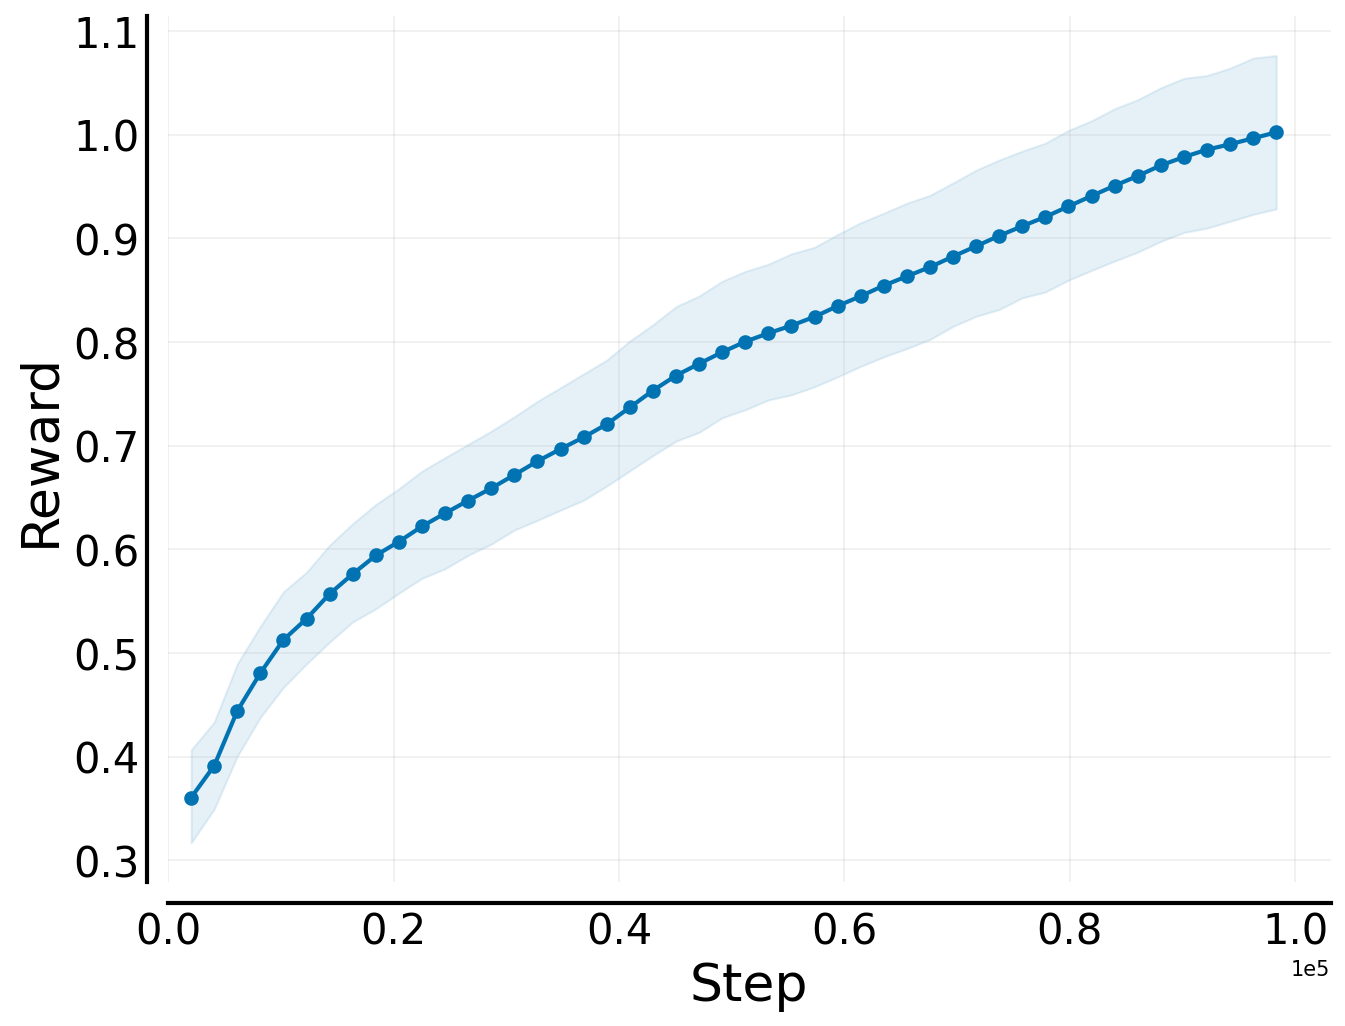
\includegraphics[width=0.35\linewidth]{figures/mazerunner/datagen.png}  
    \caption{Learning curves for data-collection runs on all 100 mazes on Maze-Runner 15$\times$15 environments with PPO-LSTM as source algorithm. We train for 100K environment steps on each maze and report the mean reward achieved (+ 95\% CI).}
    \label{fig:mazerunner-datagen}
\end{figure}

\subsection{Meta-World}\label{appendix:env-data-meta-world}
The Meta-World benchmark \citep{Yu:20} consists of 50 challenging robotics tasks, such as opening/closing a window, using a hammer, or pressing buttons. 
All tasks in Meta-World use a Sawyer robotic arm simulated using the MuJoCo physics engine \citep{Todorov:12}.
The observations and actions are 39-dimensional and 6-dimensional continuous vectors, respectively.
As all tasks share the robotic arm, the state and action spaces remain constant across tasks. 
All actions are in the range $[-1,1]$.
The reward functions are dense and based on distances to the goal locations (exact reward definitions are provided in \citet{Yu:20}).
Similar to \citet{Wolczyk:21} and \citet{Schmied:23}, we limit the episode lengths to 200 interactions.
We follow \citet{Yu:20} and split the 50 Meta-World tasks into 45 training tasks (ML45) and 5 evaluation tasks (ML5). 
During evaluation, we use deterministic environment resets after episodes, i.e., objects and goal positions are reset to their original state.
Furthermore, we mask out the goal positions in the state vector, which forces agents to adapt during environment interaction.
Agents are given 30 ICL trials during evaluation.
The 5 evaluation tasks are: 

\hspace{2.5cm}\texttt{bin-picking}, \texttt{box-close}, \texttt{door-lock}, \texttt{door-unlock}, \texttt{hand-insert}

\textbf{Training Dataset}.
For our Meta-World experiments, we leverage the datasets released by \citet{Schmied:23}. 
The datasets contain 2M transitions per task, which amounts to 90M transitions across all ML45 training tasks.
The data was generated with randomized object and goal positions after every episode. 

\subsection{DMControl}\label{appendix:env-data-dmcontrol}
DMControl contains 30 different robotic tasks with different robot morphologies \citep{Tassa:18}.
Similar to prior work \citep{Hafner:19,Schmied:23}, we select 16 of these 30 tasks and split them into 11 training (DMC11) and 5 evaluation tasks (DMC5).
The DMC11 training tasks are: 

\texttt{finger-turn\_easy}, \texttt{fish-upright}, \texttt{hopper-stand},
\texttt{point\_mass-easy},\texttt{ walker-stand}, \texttt{walker-run}, \texttt{ball\_in\_cup-catch},
\texttt{cartpole-swingup}, \texttt{cheetah-run}, \texttt{finger-spin}, \texttt{reacher-easy}

The DMC5 evaluation tasks are:

\texttt{cartpole-balance}, \texttt{finger-turn\_hard}, \texttt{pendulum-swingup}, \texttt{reacher-hard}, \texttt{walker-walk}

States and actions in DMControl are continuous vectors.
As DMControl contains different robot morphologies, the state and action spaces vary considerably across tasks ($3\leq|\mathcal{S}|\leq 24$, $1\leq|\mathcal{A}|\leq6$). 
All actions in DMControl are bounded by $[-1,1]$.
Episodes last for 1000 environment steps, and per time-step, a maximum reward of +1 can be achieved, which results in a maximum reward of 1000 per episode. 
Agents are given 30 ICL trials per task during evaluation, which results in 30K steps for a single evaluation run.  

\textbf{Training Dataset}.
As for Meta-World, we leverage the datasets released by \citet{Schmied:23}.
The datasets contain 1M transitions per task, which amounts to 11M transitions used for training across all DMC11 tasks. We refer to \citet{Schmied:23} for further dataset statistics on DMControl and Meta-World.

\subsection{Procgen}\label{appendix:env-data-procgen}
The Procgen benchmark consists of 16 procedurally-generated video games and was designed to test the generalization abilities of RL agents \citep{Cobbe:20}.
Unlike other environments considered in this work, Procgen environments emit $3\times64\times64$ images as observations.
All 16 environments share a common action space of 15 discrete actions.
The procedural generation in Procgen is controlled by setting an environment seed. 
The environment's seed randomizes the background and colour of the environment, but retains the same game dynamics.
This results in visually diverse observations for the same underlying task, as illustrated in Figure \ref{fig:procgen-seeds} for three seeds on the game \texttt{starpilot}.
The rewards in Procgen can be dense or sparse depending on the environment.

We follow \citet{Raparthy:23} and use 12 tasks for training and 4 tasks for evaluation, which we refer to as PG12 and PG4, respectively.
The PG12 tasks are:

\texttt{bigfish}, \texttt{bossfight}, \texttt{caveflyer}, \texttt{chaser}, \texttt{coinrun}, \texttt{dodgeball},\\
\texttt{fruitbot}, \texttt{heist}, \texttt{leaper}, \texttt{maze}, \texttt{miner}, \texttt{starpilot}

The PG4 tasks are: \texttt{climber}, \texttt{ninja}, \texttt{plunder}, \texttt{jumper}

We exploit the procedural generation of Procgen and evaluate all models in three settings: (1) training tasks - seen seed (PG12-Seen), (2) training tasks - unseen seed (PG12-Unseen), and (3) evaluation tasks - unseen seed (PG4).
In particular, the agents observe data from 200 different training seeds.
To enable ICL to the same environment, we always keep the same seed during evaluation (seed=1 for PG12-seen, seed=200 for PG12-Unseen and PG4).
During evaluation, we limit the episode lengths to 400 steps. 

\begin{figure}[h]
    \centering
    \subfigure[\texttt{starpilot}, seed=1]{
        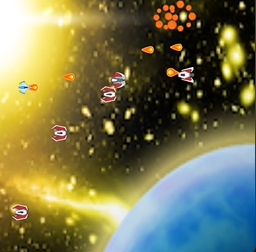
\includegraphics[width=0.25\linewidth]{figures/envs/procgen-starpilot2.png}
        \label{Startpilo}
    }
    \hspace{0.5cm}
    \subfigure[\texttt{starpilot}, seed=2]{
        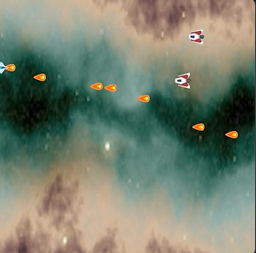
\includegraphics[width=0.25\linewidth]{figures/envs/procgen-starpilot1.png}
        \label{fig:X}
    }
    \hspace{0.5cm}
    \subfigure[\texttt{starpilot}, seed=3]{
        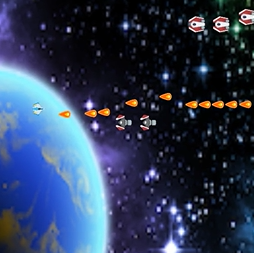
\includegraphics[width=0.25\linewidth]{figures/envs/procgen-starpilot3.png}
        \label{fig:X}
    }
    \caption{Illustration of procedural generation in Procgen \texttt{starpilot}. For different seeds, the same environment looks visually considerably different. We train on a multi-task dataset of 12 Procgen tasks, with each dataset containing trajectories from 200 environment seeds. To test for ICL, we evaluate on single hold-out seeds.}
    \label{fig:procgen-seeds}
\end{figure}

\textbf{Training Dataset.}
We generate datasets by training task-specific PPO agents for 25M timesteps on 200 environment seeds per task in \texttt{easy} difficulty, as proposed by \citet{Cobbe:20}.
We train PPO using the same hyperparameter settings as \citet{Cobbe:20}, using a learning rate of $5e^{-4}$, batch size 2048, number of update epochs of 3, entropy coefficient of $0.01$, GAE $\lambda=0.95$, and with reward normalization.
We use 256 timesteps per rollout over 64 parallel environments, which results in 16384 environment steps per rollout in total. 
Furthermore, we found it useful to decrease the discount factor to 0.99.

As in previous experiments, we record the entire replay buffer and consequently, the datasets contain mixed-quality behaviour.
We subsample the 25M transitions per task by storing only the observations of the first 5 parallel environments, which results in approximately 2M transitions per task. 
To ensure disk-space efficiency, all trajectories are stored in separate \texttt{hdf5} files in the lowest compression level, with all image-observations encoded in \texttt{unit8}.
Consequently, the datasets for all 16 tasks (32M transitions) take up only 70GB of disk space, and their \texttt{hdf5} format enables targeted reading from disk, without loading an entire trajectory into RAM.
We release two versions of our datasets: a smaller one containing 2M transitions per task as used in our experiments, and a larger one containing 20M transitions per task.

\textbf{Source Algorithm performance.}
We show the individual learning curves for all tasks in Figure \ref{fig:appendix-datacollection-procgen}, and the aggregate statistics over all 16 datasets in Table \ref{tab:procgendata}. 


\begin{table}[]
    \centering
    \caption{Dataset Statistics for all 16 Procgen tasks.}
    \begin{tabular}{l c c c}
    \toprule
    \textbf{Task} & \textbf{\# of Trajectories} &  \textbf{Mean Length}  & \textbf{Mean Return} \\
    \midrule
     \texttt{bigfish} &      8834 &    $221\pm184$ &  $ 5.9 \pm  9.1$\\
   \texttt{bossfight} &     12103 &    $161\pm200$ &  $ 2.2 \pm  4.3$\\
   \texttt{caveflyer} &     16466 &    $119\pm202$ &  $ 7.6 \pm  4.4$\\
      \texttt{chaser} &      9182 &    $213\pm72$  &  $ 3.4 \pm  3.2$\\
     \texttt{climber} &     11392 &    $171\pm248$ &  $ 9.2 \pm  5.2$\\
     \texttt{coinrun} &     38236 &     $51\pm49$  &  $ 9.7 \pm  1.8 $\\
   \texttt{dodgeball} &     13089 &    $149\pm214$ &  $ 3.2 \pm  4.2$\\
    \texttt{fruitbot} &      6966 &    $280\pm152$ &  $17.0 \pm 14.3 $\\
       \texttt{heist} &      8090 &    $241\pm395$ &  $ 8.0 \pm  4.0$\\
      \texttt{jumper} &     45621 &     $43\pm143$ &  $ 8.7 \pm  3.3$\\
      \texttt{leaper} &     28383 &     $69\pm84$  &  $ 4.9 \pm  5.0$\\
        \texttt{maze} &     48867 &     $40\pm112$ &  $ 9.5 \pm  2.3$\\
       \texttt{miner} &     26897 &     $73\pm182$ &  $11.7 \pm  3.5 $\\
       \texttt{ninja} &     24268 &     $80\pm136$ &  $ 7.8 \pm  4.2$\\
     \texttt{plunder} &      6179 &    $316\pm106$ &  $ 4.9 \pm  3.2$\\
   \texttt{starpilot} &      9490 &    $206\pm137$ &  $17.3 \pm 16.4 $\\
    \midrule
     Average &  19628 & 152 &  8.2\\
    \bottomrule
    \end{tabular}
    \label{tab:procgendata}
\end{table}

\begin{figure}
  \centering
    \subfigure{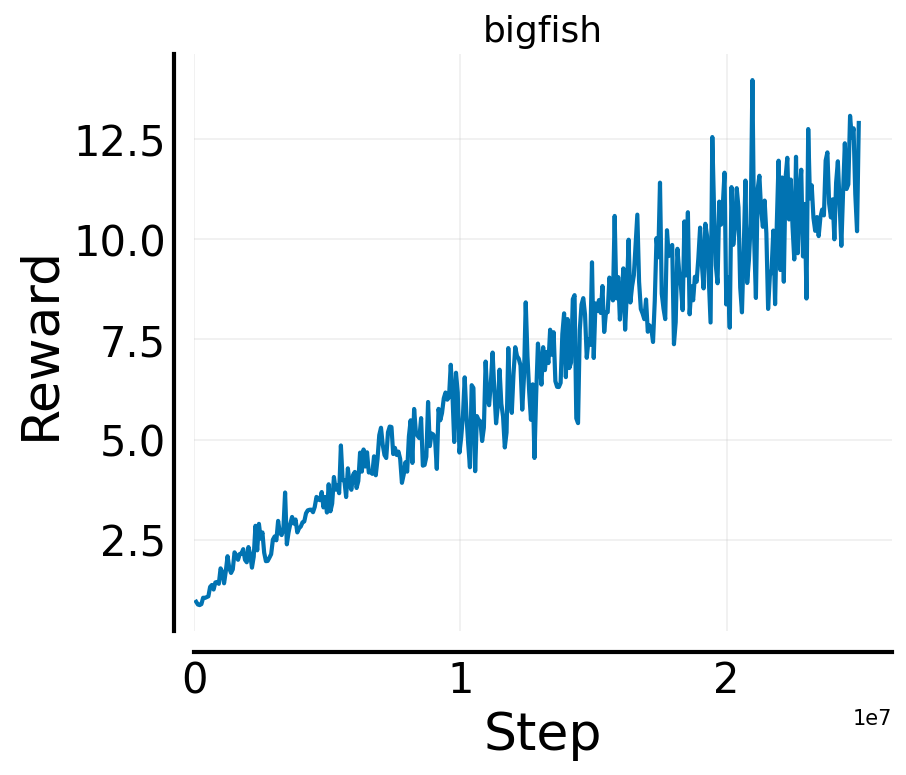
\includegraphics[width=0.24\textwidth]{figures/procgen/datagen/lc_rliable_bigfish_nolegend.png}}
    \subfigure{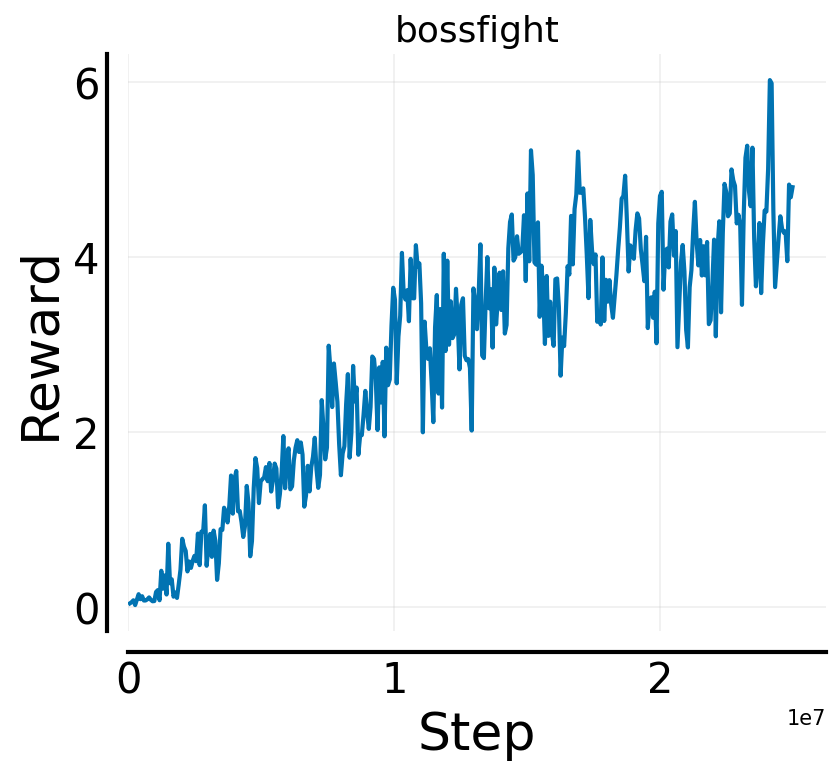
\includegraphics[width=0.24\textwidth]{figures/procgen/datagen/lc_rliable_bossfight_nolegend.png}}
    \subfigure{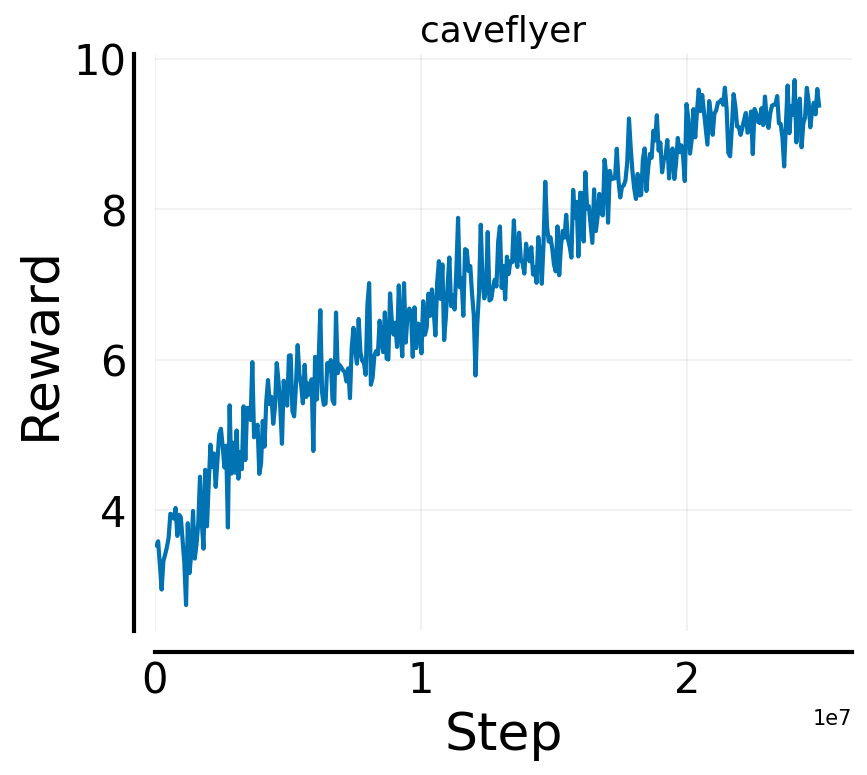
\includegraphics[width=0.24\textwidth]{figures/procgen/datagen/lc_rliable_caveflyer_nolegend.png}}
    \subfigure{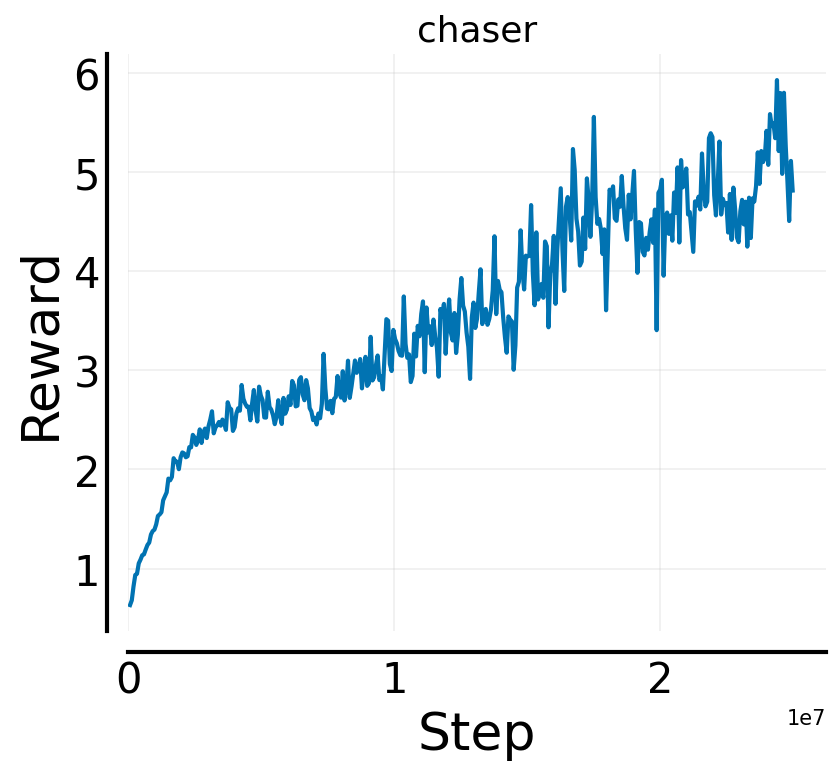
\includegraphics[width=0.24\textwidth]{figures/procgen/datagen/lc_rliable_chaser_nolegend.png}}

    
    \subfigure{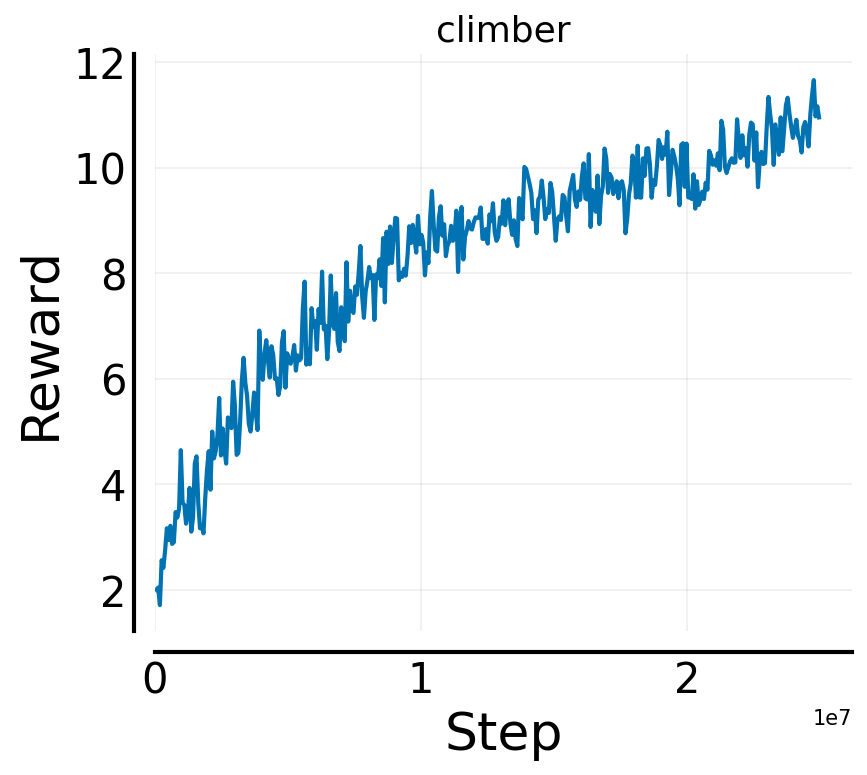
\includegraphics[width=0.24\textwidth]{figures/procgen/datagen/lc_rliable_climber_nolegend.png}}
    \subfigure{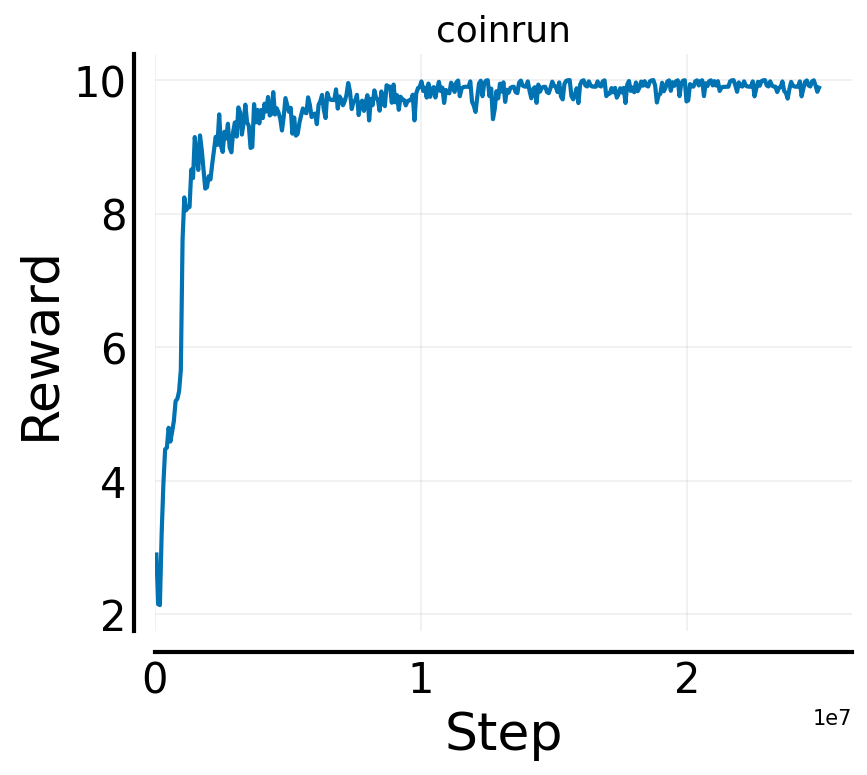
\includegraphics[width=0.24\textwidth]{figures/procgen/datagen/lc_rliable_coinrun_nolegend.png}}
    \subfigure{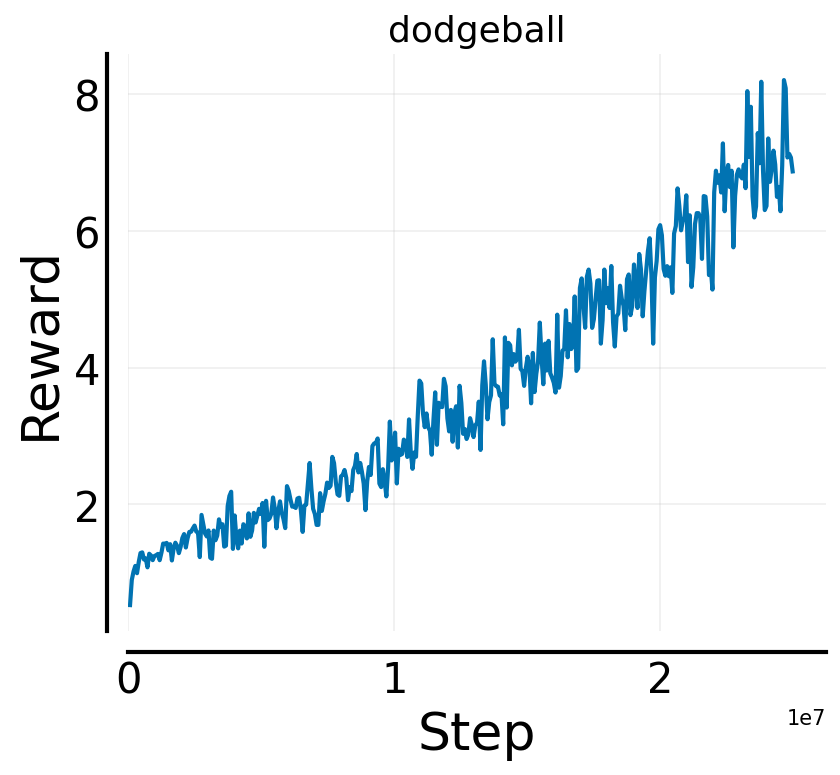
\includegraphics[width=0.24\textwidth]{figures/procgen/datagen/lc_rliable_dodgeball_nolegend.png}}
    \subfigure{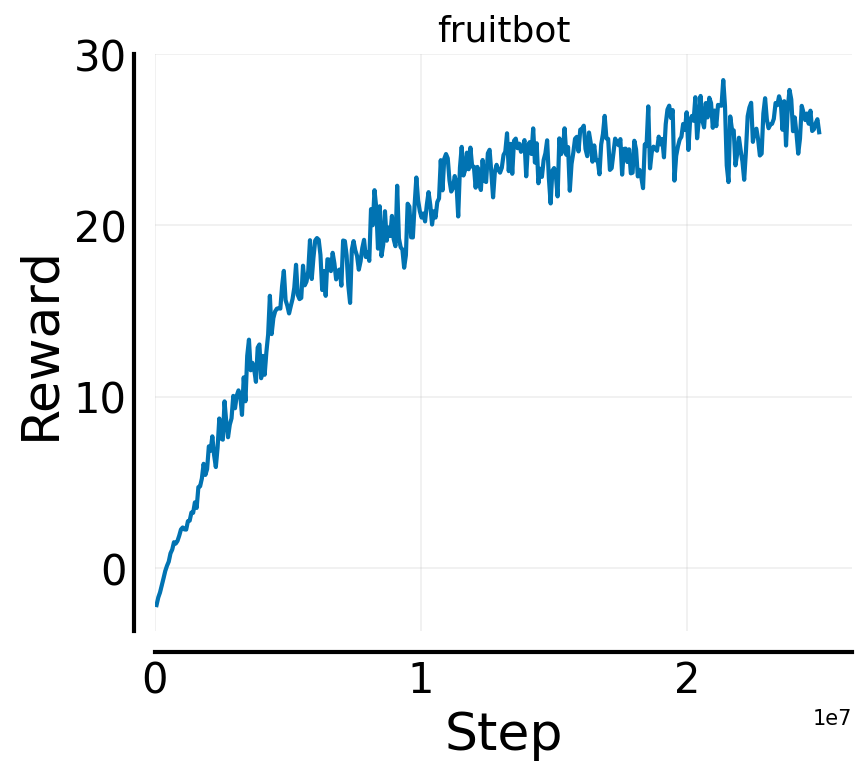
\includegraphics[width=0.24\textwidth]{figures/procgen/datagen/lc_rliable_fruitbot_nolegend.png}}

    \subfigure{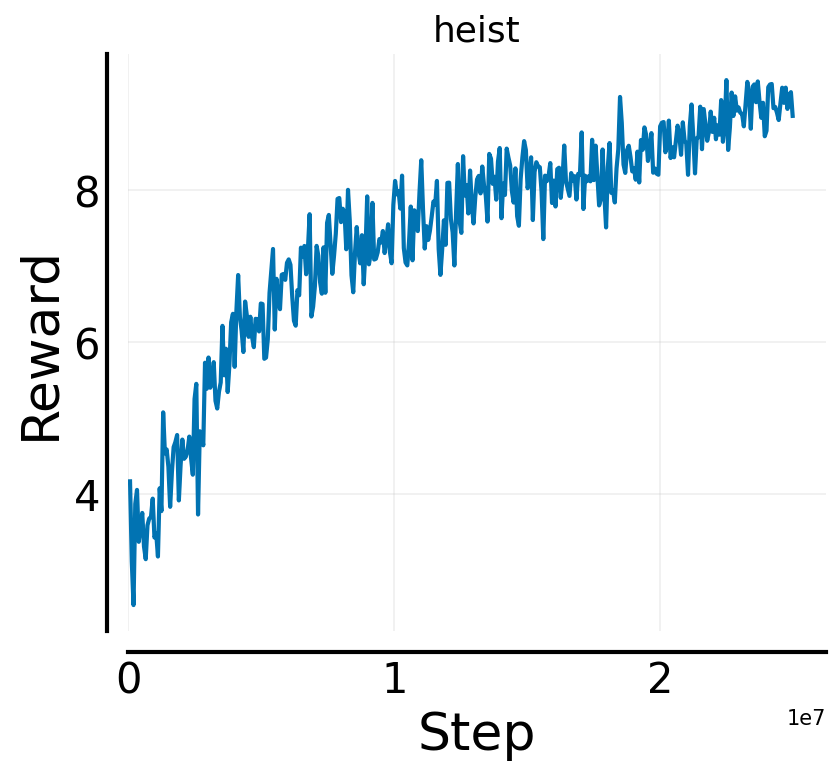
\includegraphics[width=0.24\textwidth]{figures/procgen/datagen/lc_rliable_heist_nolegend.png}}
    \subfigure{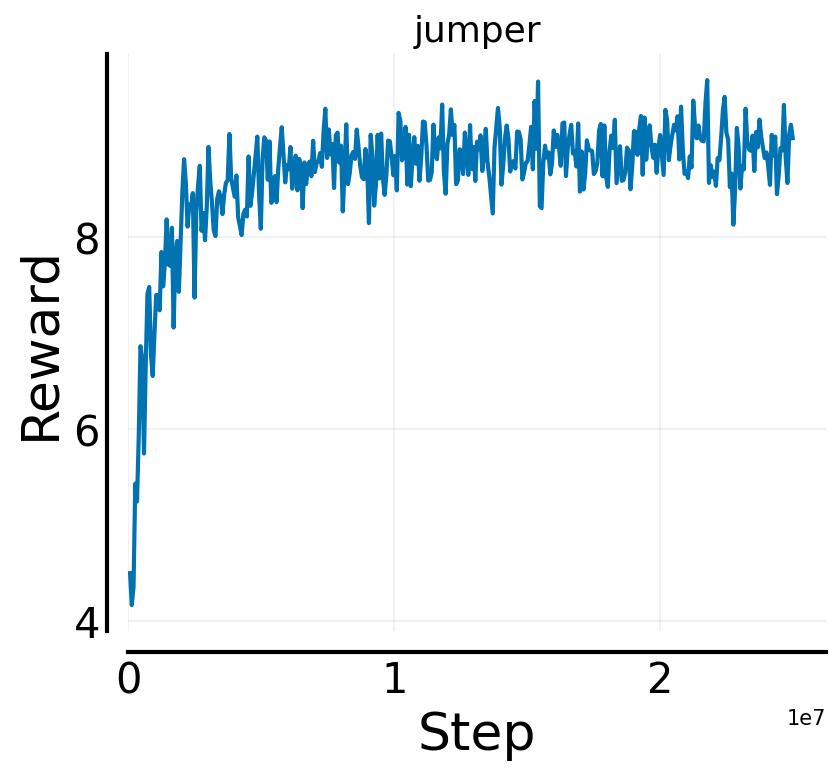
\includegraphics[width=0.24\textwidth]{figures/procgen/datagen/lc_rliable_jumper_nolegend.png}}
    \subfigure{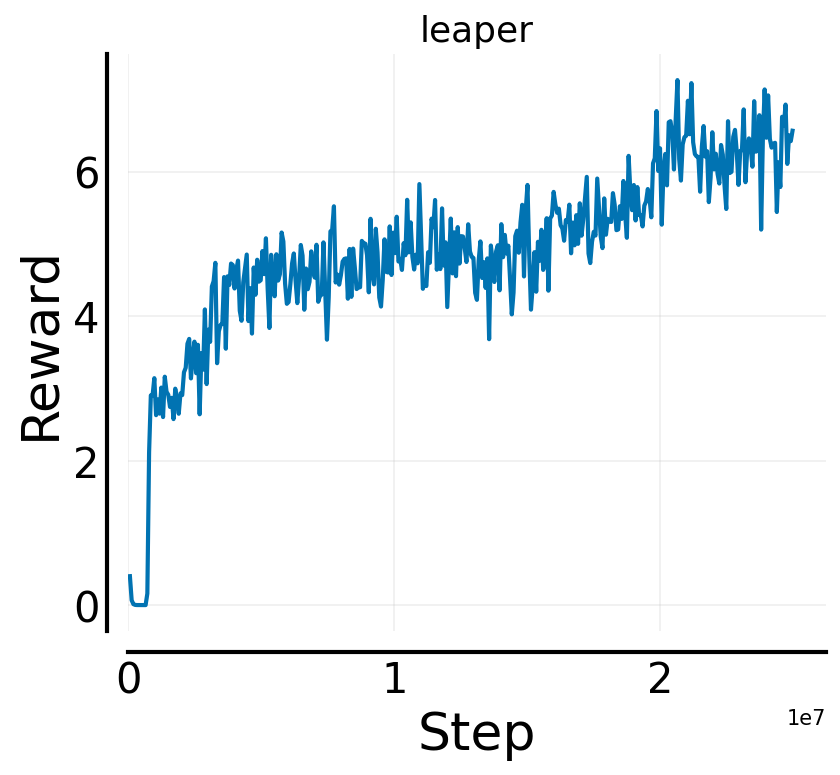
\includegraphics[width=0.24\textwidth]{figures/procgen/datagen/lc_rliable_leaper_nolegend.png}}
    \subfigure{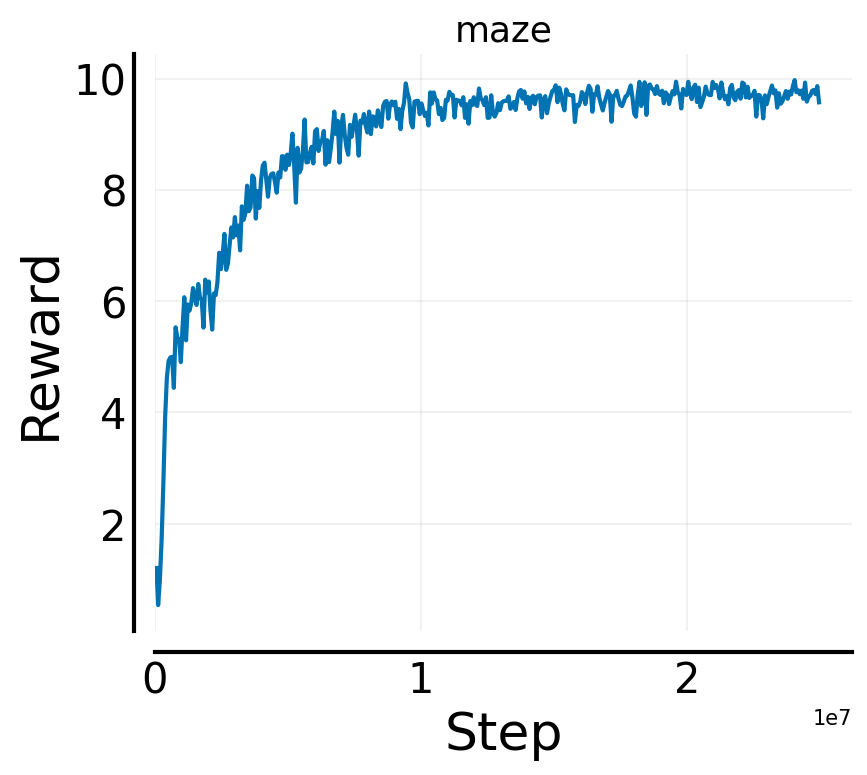
\includegraphics[width=0.24\textwidth]{figures/procgen/datagen/lc_rliable_maze_nolegend.png}}
    
    \subfigure{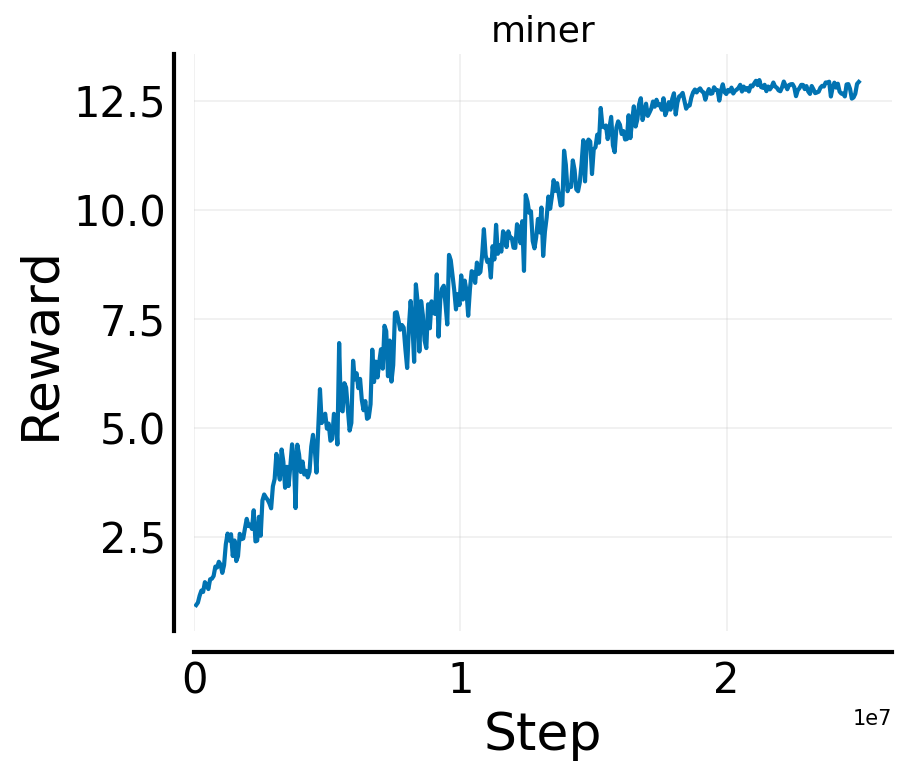
\includegraphics[width=0.24\textwidth]{figures/procgen/datagen/lc_rliable_miner_nolegend.png}}
    \subfigure{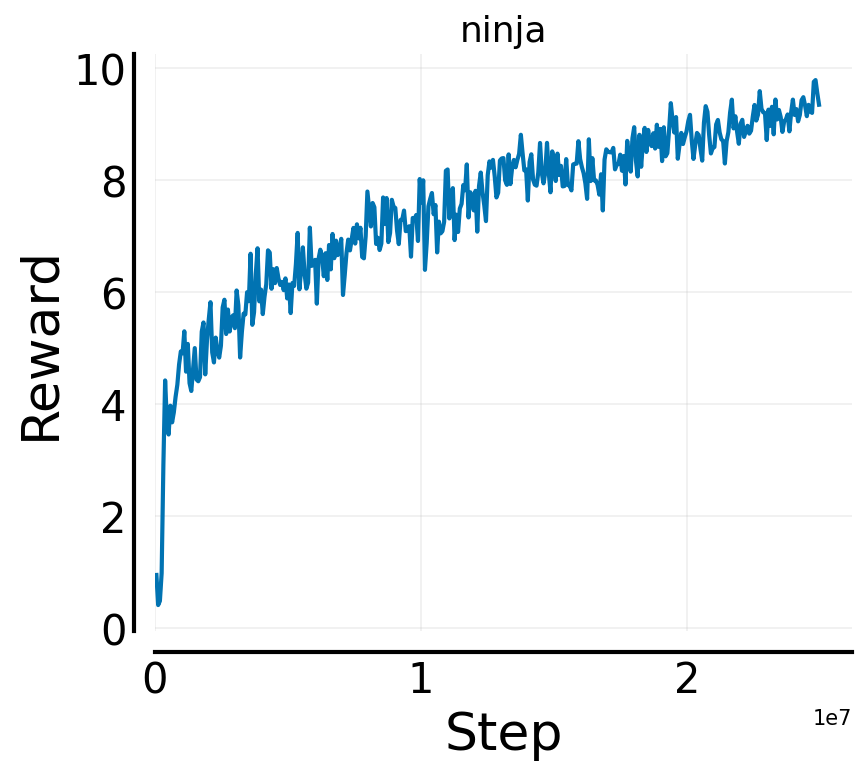
\includegraphics[width=0.24\textwidth]{figures/procgen/datagen/lc_rliable_ninja_nolegend.png}}
    \subfigure{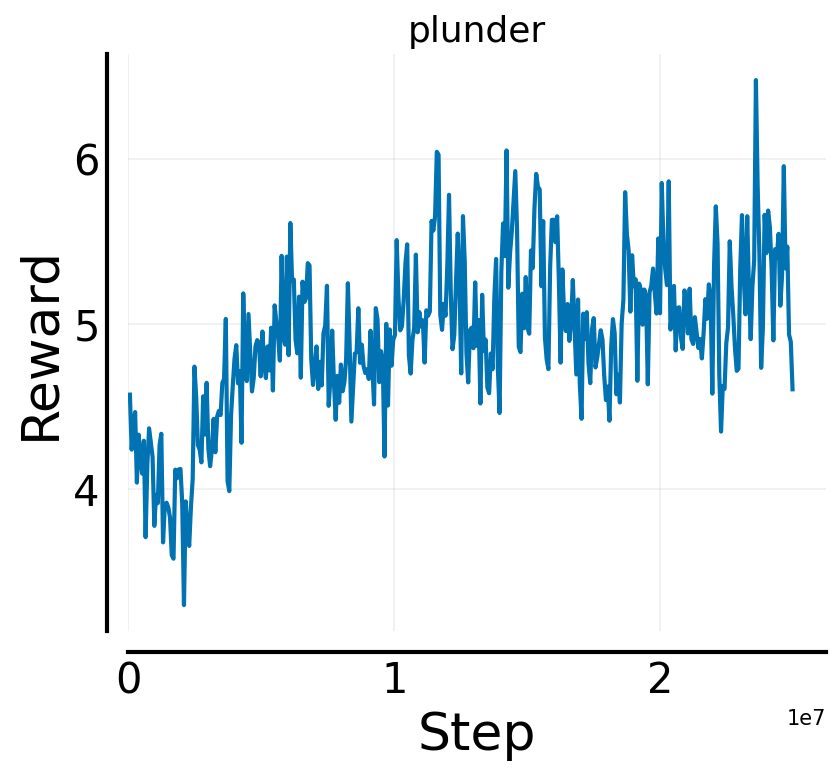
\includegraphics[width=0.24\textwidth]{figures/procgen/datagen/lc_rliable_plunder_nolegend.png}}
    \subfigure{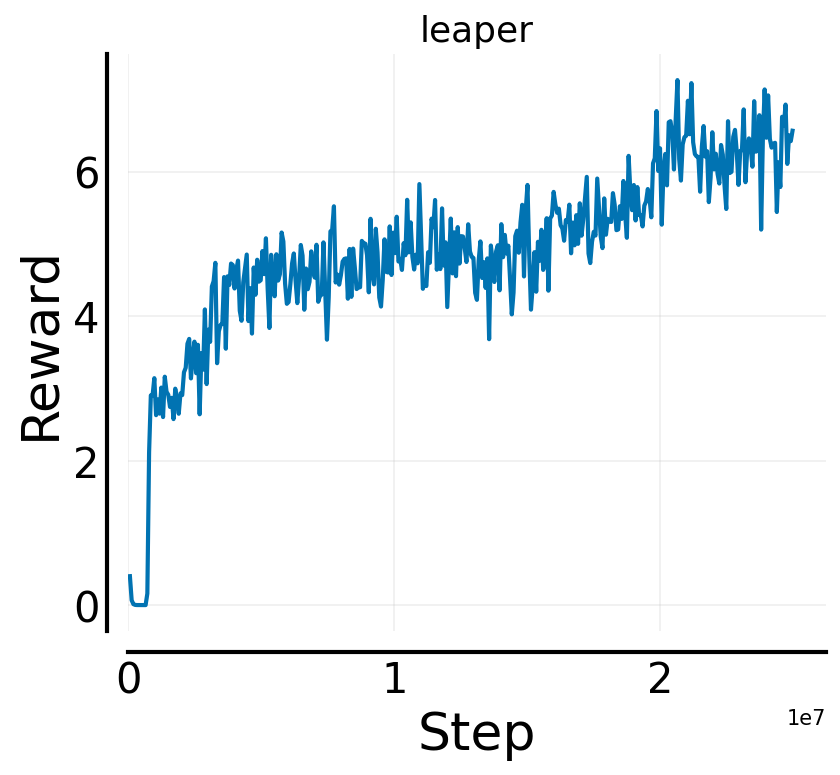
\includegraphics[width=0.24\textwidth]{figures/procgen/datagen/lc_rliable_leaper_nolegend.png}}
    
    \subfigure{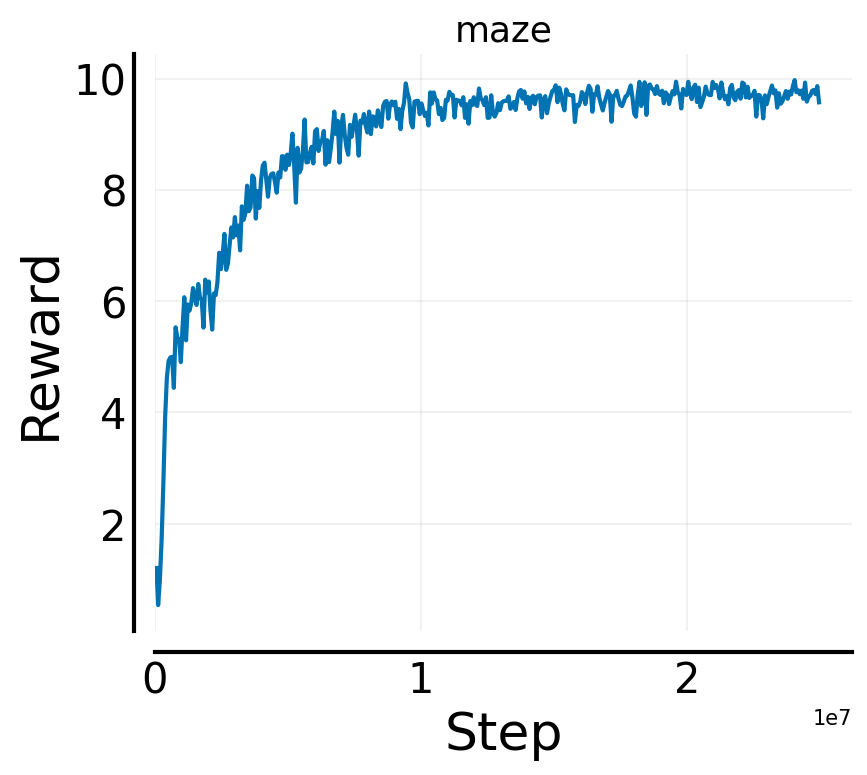
\includegraphics[width=0.24\textwidth]{figures/procgen/datagen/lc_rliable_maze_nolegend.png}}
    \subfigure{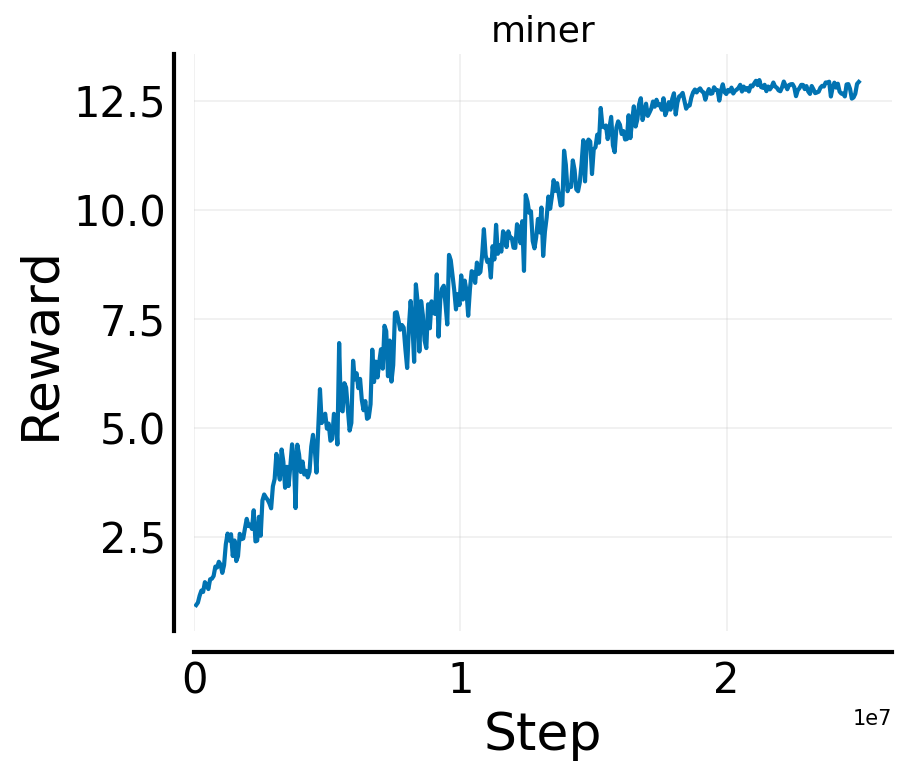
\includegraphics[width=0.24\textwidth]{figures/procgen/datagen/lc_rliable_miner_nolegend.png}}
    \subfigure{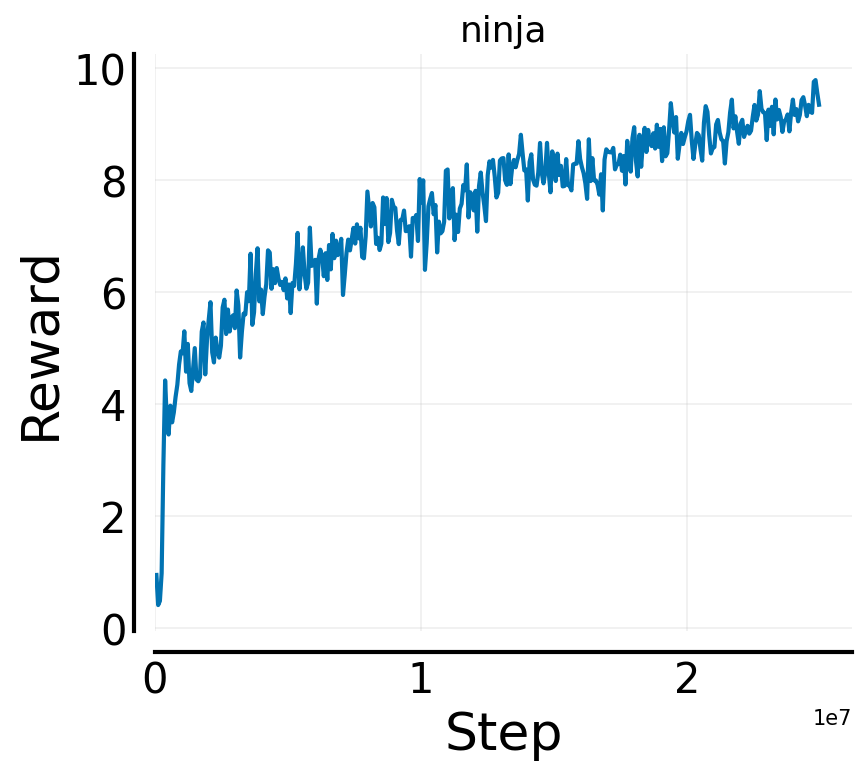
\includegraphics[width=0.24\textwidth]{figures/procgen/datagen/lc_rliable_ninja_nolegend.png}}
    \subfigure{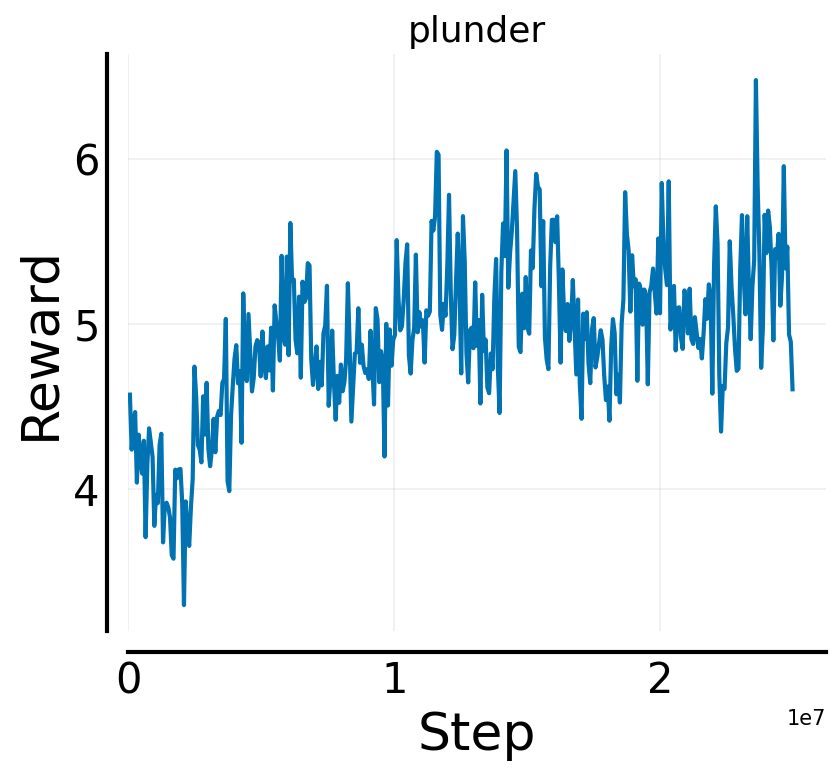
\includegraphics[width=0.24\textwidth]{figures/procgen/datagen/lc_rliable_plunder_nolegend.png}}
  \caption{Learning curves for data-collection runs on all 16 Procgen environments with PPO as source algorithm. We train for 25M environment steps on each task in \texttt{easy} mode.} 
  \label{fig:appendix-datacollection-procgen}
\end{figure}

\clearpage
\section{Experimental \& Implementation Details} \label{appendix:expdetails}
\subsection{General}\label{appendix:general}

\textbf{Training \& Evaluation.}
We compare RA-DT against DT, AD, and DPT on all environments. 
In grid-world environments, we train all methods for 100K steps and evaluate after every 25K steps. 
For Meta-World, DMControl, and Procgen, we train for 200K steps and evaluate after every 50K steps. 
During evaluation, the agent is given 40 interaction episodes for ICL on Dark-Room and Dark Key-Door, and 30 episodes on MazeRunner, Meta-World, DMControl, and Procgen.
We use the ICL curves as the primary evaluation mechanism, and report the scores at the last evaluation step (100K or 200K).
Following \citet{Agarwal:21}, we report the mean and 95\% stratified bootstrap confidence intervals across tasks and over three seeds in all experiments. 
To construct the CI bands for the learning curves, we use percentile bootstrap and 2K bootstrap samples, as suggested by \cite{Agarwal:21}.
In contrast to \citet{Agarwal:21}, we do not report the interquartile mean in our experiments, but instead opt for the mean to report in line with prior in-context RL methods \citep{Laskin:22,Lee:23}. 
Note that the evaluations conducted in this work are computationally costly because of the multi-task settings and environments with long episodes.
Therefore, we limit our experiments to three seeds per method.
Given the large number of experiments we report in this work in over 800 tasks (3 variants of Dark-Room with 100 rooms each, 3 variants of Dark Key-Door with 100 rooms, 120 mazes for MazeRunner, 50 Meta-World tasks, 16 DMControl tasks, 16 Procgen tasks) for 5 methods, increasing the number of seeds would have exceeded our computational budget. 

Across experiments, we keep most parameters fixed, unless mentioned otherwise.
We train with a batch size of 128 on all environments, except for $40\time20$ grids, where we use a batch size of 32.
We use a constant learning rate of $1e^{-4}$ and 4000 linear warm-up steps followed by a cosine decay to $1e^{-6}$ and train using the AdamW optimizer \citep{Loshchilov:18}.
Furthermore, we employ gradient clipping of 0.25, weight decay of 0.01, and a dropout rate of 0.2 for all methods.

\textbf{Context Length.} 
On grid-worlds, we use a context length $C$ equivalent to two 2 episodes for AD, DPT, and DT. 
For example, on $40\times20$ grids, this results in a sequence length of 6400 ($=1600 * 4$ for state/action/reward/RTG) for the DT and a sequence length of 4800 for AD.
On Meta-World, DMControl, and Procgen, we reduce the sequence context length to 50 steps for DT. 
For RA-DT, we use a shorter context length of $C=50$ transitions across environments, except for $20\times20$ and  $40\times20$ grids, where we increase the context length to 100.
We want to highlight that the context length for RA-DT applies to both the input context and the retrieved context. 
The retrieved context contains the past and future context, as described in Section \ref{sec:vector-index}. 
Consequently, the effective context length of RA-DT is $C+2*C$ and is independent of the episode length. 

\textbf{Network Architecture.} 
For all environments, except for Procgen, we use a GPT2-like network architecture \citep{Radford:19} with 4 Transformer layers, 8 heads, and a hidden dimension of 512, which results in 16M parameters.
On Procgen, we use a larger model with 6 Transformer blocks, 12 heads, and a hidden dimension of 768.
States, actions, rewards, and RTGs are embedded using separate embedding layers per modality, as proposed by \citet{Chen:21}.
For all modalities and environments, we use standard linear layers to embed the inputs. 
Procgen is again an exception, where we use the convolutional architecture proposed by \citet{Espeholt:18} and adopted in prior works \citep{Cobbe:20,Schmidt:21,Schwarzer:23}. 
Processing image sequences is computationally demanding. 
Therefore, we first pre-train the vision encoder using a separate DT and embed all images in the dataset using the learned vision encoder. 
Therefore, the data-loading is not bottlenecked by loading entire images into memory, but only their compact representations.

Furthermore, we use global positional embeddings.
We also experimented with the Transformer++ recipe (RoPE, SwiGLU, RMSNorm), but only observed minimal performance gains for our problem setting.
To speed up training, we use mixed-precision \cite{micikevicius2017mixed}, model compilation as supported in PyTorch \citep{Paszke:19}, and FlashAttention \citep{Dao:23}. 

\textbf{Implementation}. 
Our implementation of the DT is based on the \texttt{transformers} library \citep{Wolf:20} and \texttt{stable-baselines3} \citep{Raffin:21}.
We integrated AD, DPT, and RA-DT on top of this implementation. 

\textbf{Hardware \& Training Times}.
We run all our experiments on a server equipped with 4 A100 GPUs.
For most of our experiments, we only use a single A100.
Depending on the environment and method used, training times range from one hour (Dark-Room, DT) to 20 hours (DMControl, AD) for a single training run. 


\subsection{Decision Transformer}\label{appendix:dt}
For Dark-Room and Dark Key-Door, we sample the target return for RTG conditioning before every episode $\cN(90,5)$, $\cN(370,10)$, and $\cN(500,10)$ for grid sizes $10\times10$,  $20\times20$, and $40\times20$, respectively.
On grid-worlds, we found that sampling the target return performs better than using a fixed target return per grid size. 
We assume this is because specifying a particular target return biases the DT towards particular goal locations.
For MazeRunner, we use a constant target return of 3. 
For Meta-World, DMControl, and Procgen, we set the target return to the maximum return achieved for a particular task in the training datasets. 
However, we also found that constant target returns per domain work decently.


\subsection{Algorithm Distillation}
AD obtains a context trajectory and learns to predict actions of an input trajectory taken $K$ episodes later.
Therefore, we tune $K$ per domain. 
On grid-worlds, we found $K=100$ to perform the best, similar to \citet{Lee:23}.
For MazeRunner and Meta-World, we set $K=1000$, and for DMControl and Procgen, we set $K=250$.


\subsection{Retrieval-Augmented Decision Transformer}\label{appendix:radt-details}
\textbf{Embedding Model.} 
For the embedding model $g(\cdot)$, we either use a DT pre-trained on the same environment with the same hyperparameters as listed in Section \ref{appendix:expdetails}, or a pre-trained and frozen LM. 
For the pre-trained LM, we use \texttt{bert-base-uncased} from the \texttt{transformers} library by default. 
BERT is an encoder-only LM with 110M parameters, vocabulary size $v=30522$, and embedding dimension of $d_{\text{LM}}=768$ \citep{Devlin:18}.
We apply FrozenHopfield with $\beta=10$ to state, action, reward, and RTG tokens (see Equation \ref{eq:frozenhopfield}). 
To achieve this, we one-hot encode all discrete input tokens, such as actions in Dark-Room/MazeRunner/Procgen or states in Dark-Room, and rewards/RTGs in the sequence before applying the FH.
For other tokens, such as continuous states/actions as in Meta-World/DMControl, we directly apply the FH. 
We evaluate other alternatives for the LM in Appendix \ref{appendix:ablations}.

\renewcommand{\algorithmicensure}{\textbf{Output:}}
\renewcommand{\algorithmicrequire}{\textbf{Input:}}
\renewcommand{\algorithmiccomment}[1]{$\triangleright$ #1}
\begin{algorithm}[H]
\caption{RA-DT at training time}
\label{alg:radt-train}
  \begin{algorithmic}[1]
    \REQUIRE DT $\pi_{\theta}$, embed model $g$, dataset $\mathcal{D}$, gradient steps $N$, context len $C$, batch size $B$, eval frequency $E$, loss function $\mathcal{L}$ (cross-entropy or MSE), \texttt{evaluate}, batch-wise procedures \texttt{retrieve}, \texttt{reweight}, and \texttt{update}
    \STATE $\mathcal{I} \gets \emptyset$ \hfill\COMMENT{Initialize retrieval index $\mathcal{I}$}
    \FOR{$\tau \in \mathcal{D}$}
        \STATE $\mathcal{I} \gets \mathcal{I} \cup \{(g(\tau_{t-C:t}), \tau_{t-C:t+C}) \mid t \in \text{range}(0, |\tau|, C)\}$ \hfill\COMMENT{Add k-v pairs of sub-trjs to $\cI$ }
    \ENDFOR
    \FOR{$i = 1 \ldots N$}
        \STATE $\mathbf{b} \sim \mathcal{D}$ where $\mathbf{b}=\{\tau_j\ \mid 1 \leq j \leq B\} $ \hfill\COMMENT{Sample batch of sub-trjs each of length $C$}
        \STATE $\mathbf{q} = g(\mathbf{b})$ \hfill\COMMENT{Construct queries for all sub-trjs}
        \STATE $\mathcal{R} \gets \text{\texttt{retrieve}}(\mathbf{q}, \mathcal{I})$ \hfill\COMMENT{Retrieve top-$l$ sub-trjs, Eq. \ref{eq:retrieve}}
        \STATE $\mathcal{S} \gets \text{\texttt{reweight}}(\mathcal{R})$ \hfill\COMMENT{Re-weight top-$k$ sub-trjs, Eq. \ref{eq:retscore}, \ref{eq:reweight}}
        \STATE $\mathbf{a} = \pi_{\theta} (\cdot \mid \mathbf{b}, \{\tau_{\text{ret}} \in \mathcal{S}\} )$ \hfill\COMMENT{Predict actions for batch}
        \STATE $\pi_{\theta} \gets \texttt{update}(\pi_{\theta}, \mathcal{L}, \mathbf{a}, \mathbf{b})$ \hfill\COMMENT{Perform gradient step, see Appendix \ref{appendix:general} for $\mathcal{L}$}
        \IF{$i \; \% \; E == 0$}
            \STATE \text{\texttt{evaluate}}($\pi_{\theta}$, $g$) \hfill\COMMENT{Evaluation with ICL, see Algorithm \ref{alg:radt-inference}}
        \ENDIF
    \ENDFOR
  \end{algorithmic}
\end{algorithm}

\textbf{Constructing queries/keys/values.}
Regardless of whether $g$ is domain-specific or domain-agnostic, we obtain $C$ embedded tokens after applying $g$ to the input trajectory $\tau_{in}$. 
Subsequently, we apply mean aggregation over the context length $C$ to obtain the $d_r$-dimensional query representation.
We experimented with aggregating over all tokens or only tokens of a particular modality (state/action/reward/RTG), and found aggregation over states-only to be most effective (see Appendix \ref{appendix:seq-agg}).
As described in Section \ref{sec:vector-index}, we construct the key-value pairs in our retrieval index by embedding all sub-trajectories in the dataset $\mathcal{D}$ using our embedding model $g$, $\cK \times \cV = \{(g(\tau_{i, t-C:t}), \tau_{i, t-C:t+C}) \mid 1 \leq i \leq |\cD| \}$.
To avoid redundancy, in practice, we construct $H / C$ key-value pairs for a given trajectory $\tau$ with episode length $H$ and sub-sequence length $C$, instead of constructing the key and values for every step $t \in [1,H]$.
Note that the values, we store $\tau_{i, t-C:t+C}$, contain both the sub-trajectory itself ($\tau_{i, t-C:t}$) and its continuation ($\tau_{i, t:t+C}$).
Similar to \citet{Borgeaud:22}, we found this choice important for high performance in RA-DT, because it allows the model to observe how the trajectory may evolve if it predicts a certain action (given that the retrieved context is similar enough).

\textbf{Vector Index.} We use Faiss \citep{Johnson:2019,Douze:2024} to instantiate our vector index $\cI$.
This allows us to search our vector index in $\mathcal{O}(\log M)$ time using Hierarchical Navigable Small World (HNSW) graphs. 
Consequently, retrieval-augmentation is highly scalable and commonly employed in LMs with large-scale datasets that contain trillions of tokens \citep{Borgeaud:22}.
For the datasets we consider, we found it faster to use a Flat index on the GPU as provided by Faiss instead of using HNSW, because our retrieval datasets are small enough.
We use retrieval both during training and during inference. 
It is, however, possible to pre-compute the retrieved trajectories for $\cD$ before the training phase to limit the computational demand of retrieval, as suggested by \citet{Borgeaud:22}.
During evaluation, we can retrieve after every environment step or only after every $t$ environment steps. 
Here, $t$ represents a trade-off between inference time and final performance. 
We use $t=1$ for Dark-Room and Dark Key-Door, and $t=25$ for all other environments (see Appendix \ref{appendix:steps-between-retrievals} for an ablation on this design choice).
For all environments, except for Meta-World and DMControl, we provide a single retrieved sub-trajectory in the agent's context. 
For Meta-World and DMControl, we found that providing more than one retrieved sub-trajectory benefits the agent's performance.
Therefore, for these two environments, we retrieve the top-4 sub-trajectories, order them by return achieved in that trajectory, and provide their concatenation as retrieved context for RA-DT. 

\textbf{Reweighting.}
To implement the reweighting mechanism, as described in Section \ref{sec:reweighting}, we first retrieve the top $l\gg k$ experiences and select the top-$k$ experiences according to their reweighted scores. 
We set $l=50$ in all our experiments.  

\begin{table}[]
    \centering
    \caption{Hyperparameters for RA-DT.}
    \begin{tabular}{l | c c}
    \toprule
    \textbf{Environment} & \textbf{Parameter} & \textbf{Value} \\
    \midrule
     Default &      Gradient steps & 100K \\
      &      Optimizer & AdamW \\
      &      Batch size & 128 \\
      &      Lr schedule & Linear warm-up + Cosine \\
      &      Warm-up steps & 4000 \\
      &      Learning rate & 1e-4 $\rightarrow$ 1e-6\\
      &      Weight decay & 0.01 \\
      &      Gradient clipping & 0.25 \\
      &      Dropout & 0.2 \\
      &      Context Length & 50 timesteps \\
      &      Top-$k$ before re-weighting & 50 \\
      &      Top-$k$ after re-weighting & 1 \\
      &      Eval steps between retrievals & 1 \\
      &      Query sequence aggregation & mean \\
      &      Query sequence tokens & state \\
      &      Query dropout & 0.2 \\
      &      Re-weight $\alpha$ & 1 \\
      &      Train re-weighting & task \\
      &      Eval re-weighting & return \\
      &      Similarity cut-off & 0.98 \\
      &      Deduplicate & True \\
      &      Min len for retrieval (only for Dark) & 10 \\
      &      Domain-agnostic LM & \texttt{bert-base-uncased} \\
      &      Domain-agnostic LM hidden dim & 768 \\
      &      FrozenHopfield $\beta$ & 10 \\
    \midrule
     Dark Room/Key-Door $20\times20$ &      Context length & 100 \\
    \midrule
     Dark Room/Key-Door $40\times20$ &      Context length & 100 \\
      &      Batch size & 32 \\
     \midrule
     MazeRunner &      Eval steps between retrievals & 25 \\
    \midrule
     Meta-World/DMControl &  Gradient steps & 200K \\
      &                      Eval steps between retrievals & 25 \\
      &      Top-$k$ after re-weighting & 4 \\
      &  Query blending                 & 0.5 \\  
    \midrule
     Procgen &      Gradient steps & 200K \\     
             &      Eval steps between retrievals & 25 \\
    \bottomrule
    \end{tabular}
    \label{tab:radt-hparams}
\end{table}

\textbf{Embedding Retrieved Context.}
After the most similar trajectories have been retrieved, we embed the state/action/reward/RTG tokens with a separate embedding layer (as is done for the regular input sequence) before incorporating them via the CA layers.
We also experimented with sharing/detaching the regular embedding layers, but found it most effective to maintain separate ones. 
Furthermore, we experimented with an additional Transformer-based encoder for the retrieved sequences, as proposed by \citet{Borgeaud:22}, but did not observe substantial performance gains despite increased computational cost.

\textbf{Retrieval Dataset.}
For all our experiments, we use the same dataset for retrieval $\mathcal{D}'$ as is used for training $\mathcal{D}$, that is $\mathcal{D}'=\mathcal{D}$.
Therefore, we prevent retrieving sub-sequences from the same trajectory as the query. 

\textbf{Retrieval Regularization.}
We found it advantageous to regularize the k-NN retrieval in RA-DT throughout the training phase.
In RL datasets, there is often a substantial overlap between trajectories, leading to many similar sub-trajectories.
This poses a significant challenge, as retrieving only similar sub-trajectories encourages the agent to adopt copying behaviour, which renders the DT unable to produce high-reward actions during inference. 

One simple strategy to mitigate this issue is \textbf{deduplication}, i.e., to discard duplicate experiences before the training phase of RA-DT.
To achieve this, we first construct our index as described in Section \ref{sec:radt}.
For every key $\mathbf{k} \in \mathbf{K}$, we retrieve the top-$k$ neighbours (excluding experiences from the same episode as $\mathbf{k}$). 
If the similarity score is above a cosine similarity of $0.98$, we discard the experience.
This substantially reduces the number of experiences in the index and speeds up retrieval.
Note that deduplication can be used at inference time to avoid storing redundant experiences.

\begin{figure*}[h]
    \centering
    
\includegraphics[width=0.75\linewidth]{figures/dark_keydoor/20x20/legend.png}  
    
    \subfigure[Dark-Room 10$\times$10]{
        
\includegraphics[width=0.31\linewidth]{figures/darkroom/10x10/train_icl.png}
        \label{fig:sub1}
    }
    \hfill
    \subfigure[Dark-Room 20$\times$20]{
        
\includegraphics[width=0.31\linewidth]{figures/darkroom/20x20/train_icl.png}
        \label{fig:sub2}
    }
    \hfill
    \subfigure[Dark-Room 40$\times$20]{
        
\includegraphics[width=0.33\linewidth]{figures/darkroom/40x20/train_icl.png}
        \label{fig:sub3}
    }
    \caption{In-context learning performance on \textbf{(a) Dark-Room 10$\times$10}, \textbf{(b) Dark-Room 20$\times$20}, \textbf{(c) Dark-Room 40$\times$20} at end of training (100K steps). We evaluate each agent for 40 episodes on each of the 80 \textbf{training tasks} and report mean reward (+ 95\% CI) over 3 seeds.}
    \label{fig:darkroom-icl-train}
\end{figure*}

Two other strategies for regularizing retrieval during the training phase are \textbf{similarity cut-off} and \textbf{query dropout} \citep{yasunaga_retrieval_2023}. 
Similarity cut-off first retrieves the top $m > l$ experiences, discards the experiences with a similarity score above a threshold (e.g., $0.98$), and retains only the remaining experiences $l$.
If used in combination with reweighting, we set $m=2*l$.
Query dropout randomly drops out tokens (e.g., 20\%) of the embedded sub-trajectory $\tau_{\text{in}}$, which leads to more diverse retrieved experiences. 
We found both strategies effective for RA-DT.
We use a query dropout of 0.2, a similarity cut-off of 0.98, and deduplication by default.
Furthermore, for Meta-World and DMControl, we found \textbf{query-blending} useful. 
Query-blending interpolates between the actual query and a randomly selected key from the retrieval index, $\Bq'=\Bq * \alpha_{\text{blend}} + (1-\alpha) \Bq_{\text{rand}}$. 
For Meta-World and DMControl, we additionally set $\alpha_{\text{blend}}=0.5$. 

On Dark-Room and Dark Key-Door environments, we found it useful to replace retrieved experiences with experiences randomly sampled from the same task if the query sub-sequence is from the beginning of the episode (i.e., smaller than timestep 10). 
This is because in these two environments, retrieving appropriate experience can be difficult if the given query sub-sequence is too short.  

Finally, we use the same RTG-conditioning strategy as the vanilla DT, as described in Appendix \ref{appendix:dt}. 

\begin{figure*}[h]
    \centering
    
\includegraphics[width=0.75\linewidth]{figures/dark_keydoor/20x20/legend.png}  
    
    \subfigure[80 Train Goals]{
        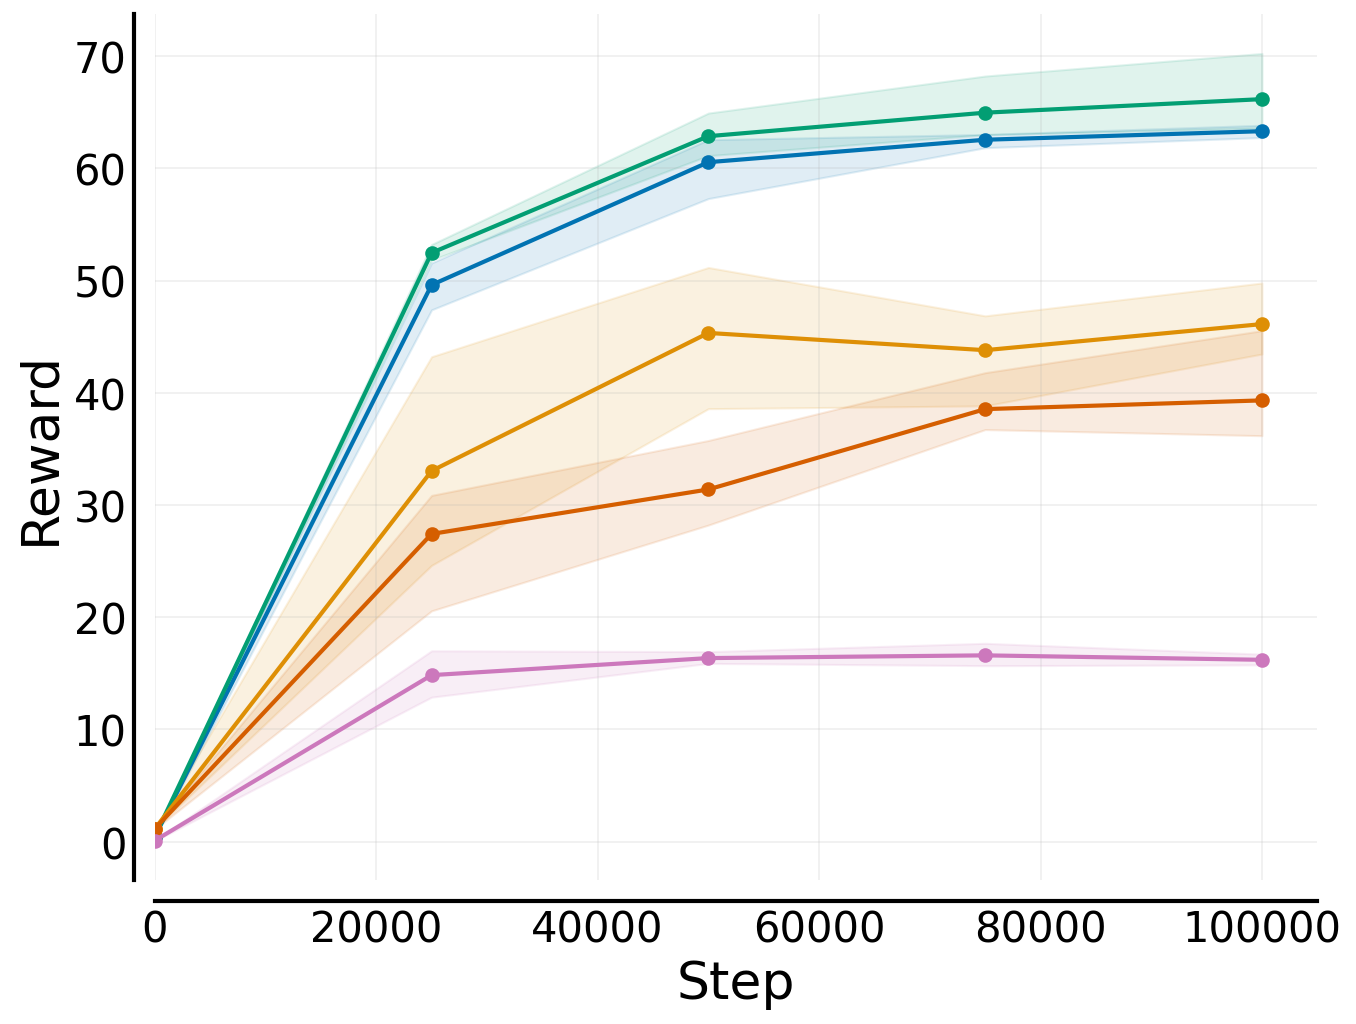
\includegraphics[width=0.31\linewidth]{figures/darkroom/10x10/train.png}
        \label{fig:sub1}
    }
    \hspace{1cm}
    \subfigure[20 Eval Goals]{
        
\includegraphics[width=0.31\linewidth]{figures/darkroom/10x10/eval.png}
        \label{fig:sub2}
    }
    \caption{Average performances on \textbf{Dark-Room 10$\times$10} over the course of training for \textbf{(a)} train and \textbf{(b)} test tasks.
    We train each agent for 100K steps and evaluate every 25K steps. Curves are averaged across the 80 training and 20 evaluation tasks, respectively. We report mean reward (+ 95\% CI) over 3 seeds.}    
    \label{fig:darkroom-train-eval-avg}
\end{figure*}

\begin{figure}[ht]
    \centering
    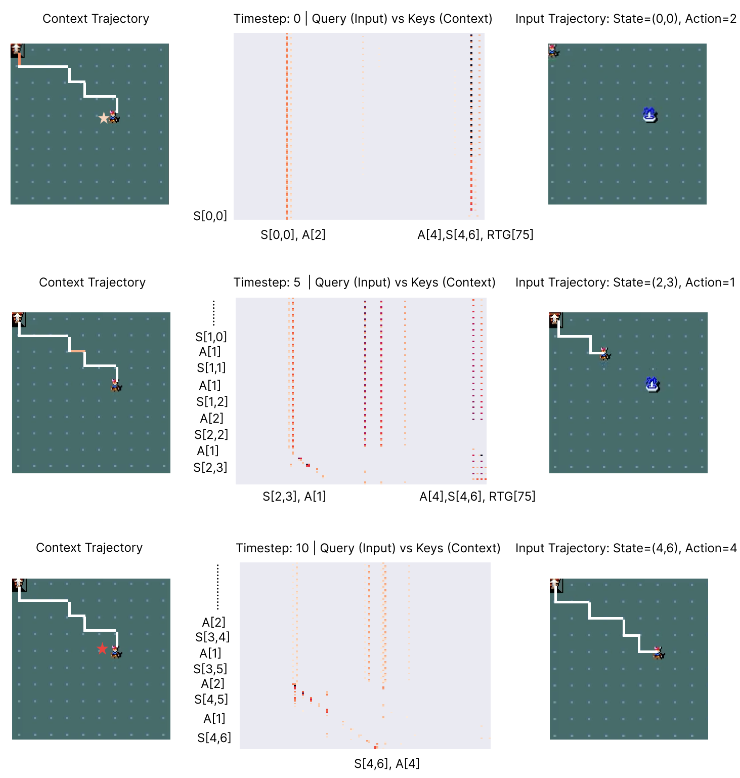
\includegraphics[width=1.0\linewidth]{figures/visualisation/positive.png}  
    \caption{Attention map analysis for an \textbf{optimal context-trajectory} on Dark-Room $10\times10$. We plot the retrieved context trajectory (left), the corresponding attention map, and the actual agent state (right), across timesteps (1, 5, 10).
    Queries (input trajectory) are on the y-axis and keys (context trajectory) on the x-axis. 
    We highlight the sub-sequence in the context trajectory with the highest attention score (left).
    To improve readability, we mask out attention scores below a certain threshold and only provide labels for tokens that exhibit the highest attention scores.
    The agent imitates the context trajectory and successfully finds the goal.}
    \label{appendix:att-map-optimal}
\end{figure}
\begin{figure}[ht]
    \centering
    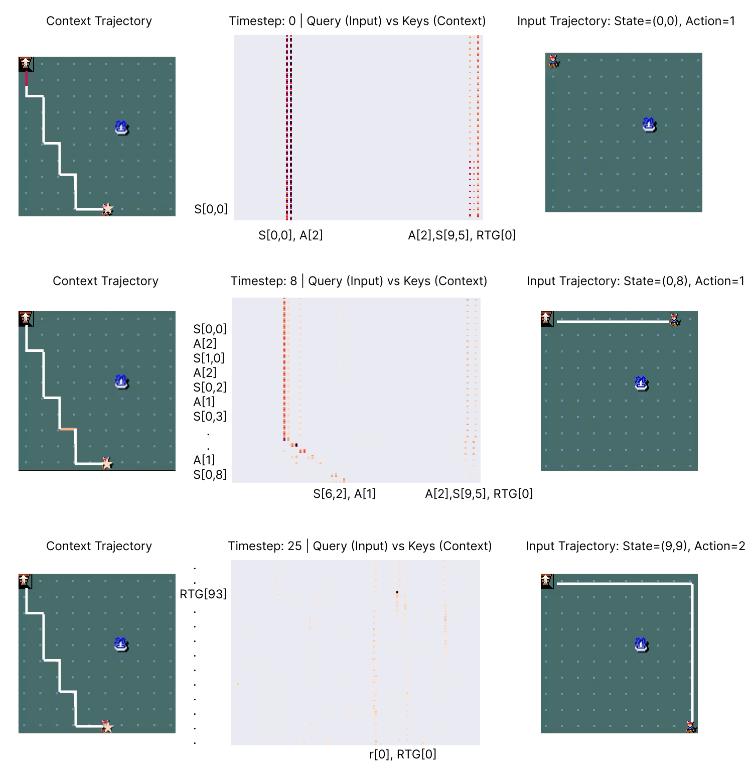
\includegraphics[width=1.0\linewidth]{figures/visualisation/negative.png}  
    \caption{
    Attention map analysis for a \textbf{suboptimal context-trajectory} on Dark-Room $10\times10$.     
    The agent selects a different route than is present in the suboptimal context trajectory and explores the environment.}
    \label{appendix:att-map-suboptimal}
\end{figure}

\clearpage
\section{Additional Results}\label{appendix:results}
\subsection{Dark-Room}\label{appendix:expdetails-darkroom}
Analogous to the ICL curves on the 20 evaluation tasks in Figure \ref{fig:darkroom-icl-eval}, we present ICL curves on the 80 train tasks in Figure \ref{fig:darkroom-icl-train}. 
In general, we observe a similar learning behaviour on the train tasks as on the evaluation tasks, with slightly higher scores on average. 
Interestingly, the domain-agnostic variant of RA-DT slightly outperforms its domain-specific counterpart on the training tasks. 

In addition, we also show the learning curves on Dark-Room $10\times 10$ over the entire training phase in Figure \ref{fig:darkroom-train-eval-avg}. 
We evaluate after every 25K updates and observe a steady improvement in the average performance with every evaluation.  

\subsubsection{Attention Map Analysis}\label{appendix:attn-maps}
We conduct a qualitative analysis on Dark-Room $10\times10$ to better understand how RA-DT leverages the retrieved context sub-sequences. 
First, we analyse the attention maps for different Dark-Room $10\times10$ goal locations.

\textbf{What happens if an optimal trajectory is retrieved in context? }
In Figure \ref{appendix:att-map-optimal}, we showcase this example. 
The goal location is located at grid cell (4,6).
The attention maps exhibit high attention scores for the state and the RTG at the end of the retrieved trajectory.
We also observe high attention scores for the state, similar to the current state and the action selected in that state. 
The agent initially imitates the actions in the context trajectory, but deviates further into the episode. 
Once the agent reaches the goal state, the attention scores for states and RTGs at the end of the trajectory reduce considerably, because the agent needs not pay attention to the retrieved context any more.


\textbf{What happens if a suboptimal trajectory is retrieved in Context?}
Similarly, we show the corresponding example in Figure \ref{appendix:att-map-suboptimal}.
The goal location is again in grid cell (4,6). 
The retrieved context trajectory reaches the final state (9,5).
Similar to Figure \ref{appendix:att-map-optimal}, the attention maps exhibit high attention scores for the last state and RTG for that state, as well as for a state at a similar timestep.
Previously, RA-DT imitated the action, but in this situation, the agent
picks a different route, as the context trajectory does not lead to a successful outcome. 

This analysis suggests that RA-DT can develop capabilities to either imitate a given positive experience or to behave differently than a given negative experience.   

\subsubsection{Exploration Analysis}
\textbf{State Visitations.}
In Section \ref{appendix:attn-maps}, we found that RA-DT learned to either copy or avoid behaviours given positive or negative context trajectories. 
Therefore, we further analyse the exploration behaviour of RA-DT by visualizing the state-visitation frequencies on Dark-Room $10\times10$ across the 40 ICL trials for three different goal locations: $(5,8)$, $(5,1)$, and $(4,6)$ (see Figure \ref{appendix:exploration}).
The agent visits nearly all states at least once at test time, as visualized in Figure \ref{appendix:exploration} (a) and (b). 
Once the agent finds the goal location, it starts to imitate and stops exploring, as illustrated in Figure \ref{appendix:exploration} (c). 

\begin{figure*}[ht]
    \centering
    \subfigure[Goal Location: (5,8)]{
        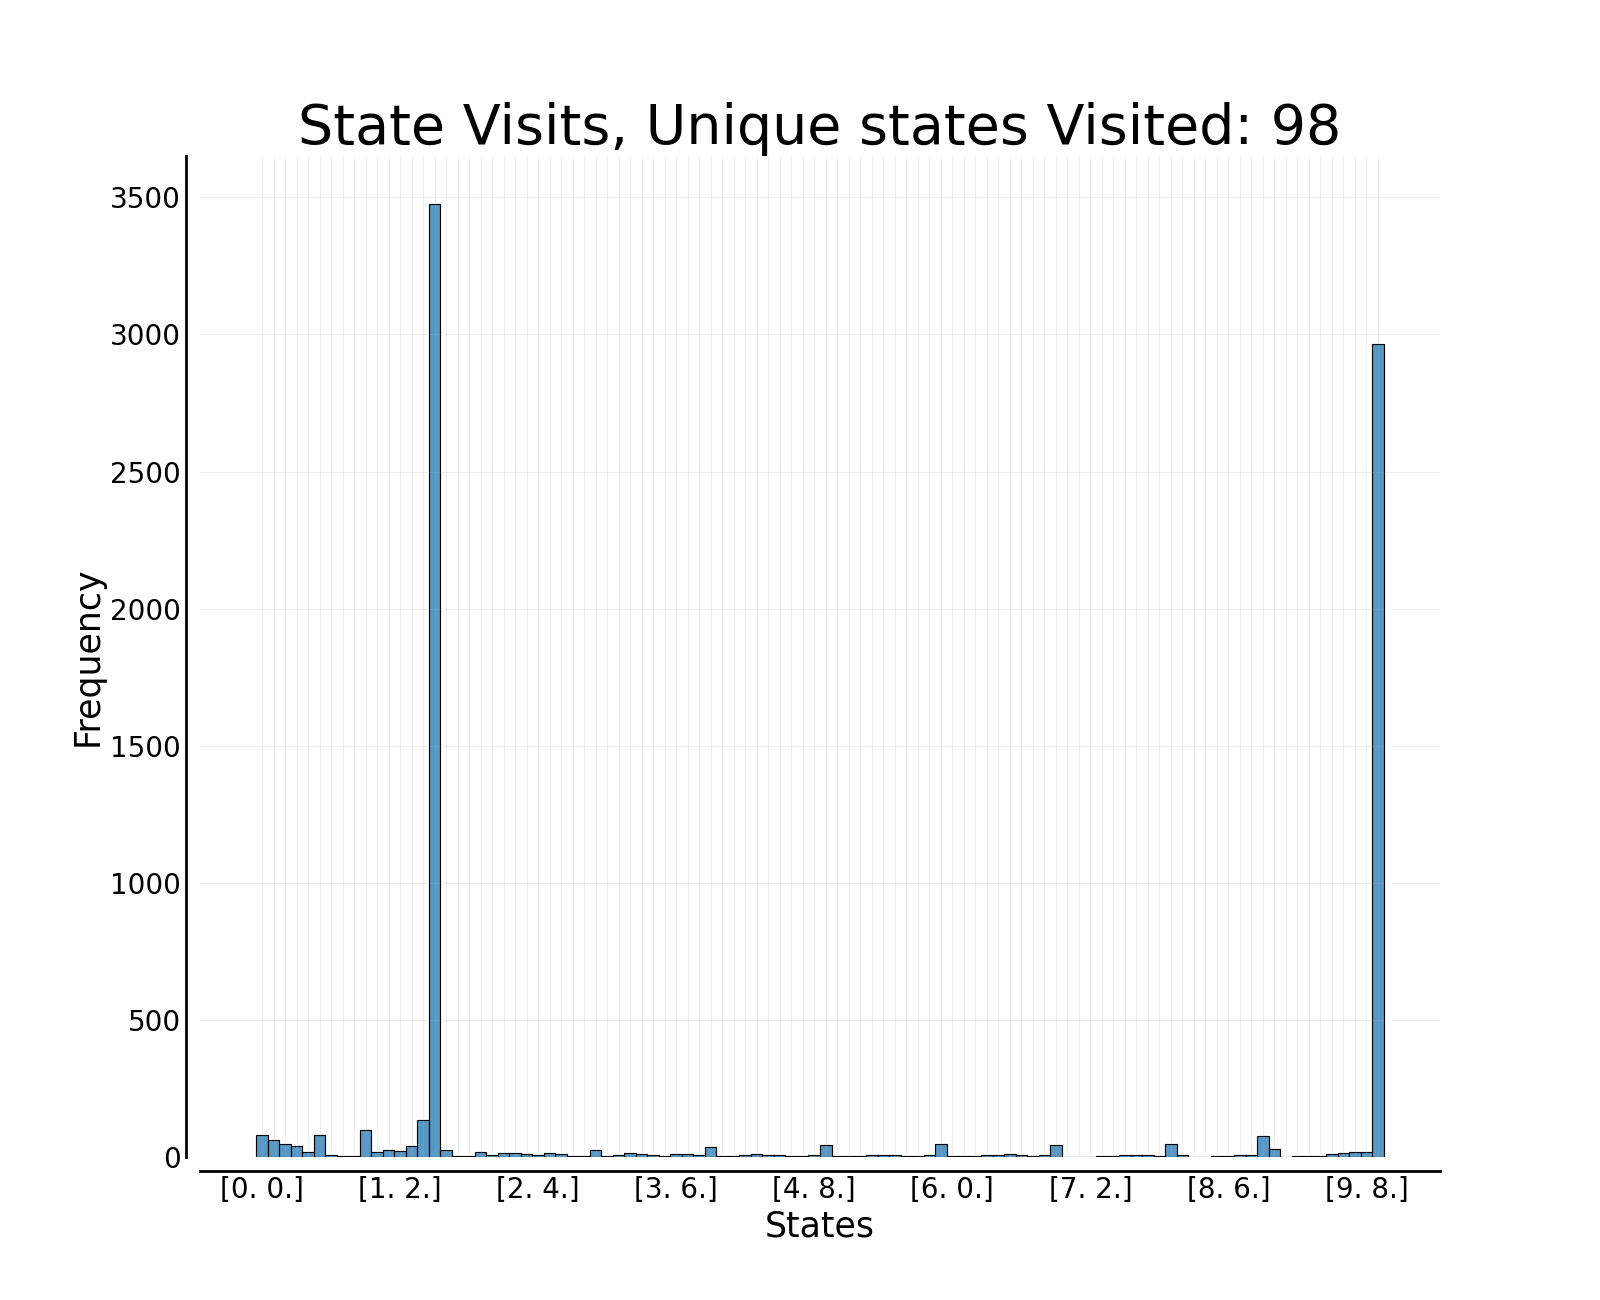
\includegraphics[width=0.31\linewidth]{figures/visualisation/state_action_coverage_RTG_84_5_8.png}
    }
    \hfill
    \subfigure[Goal Location: (5,1)]{
        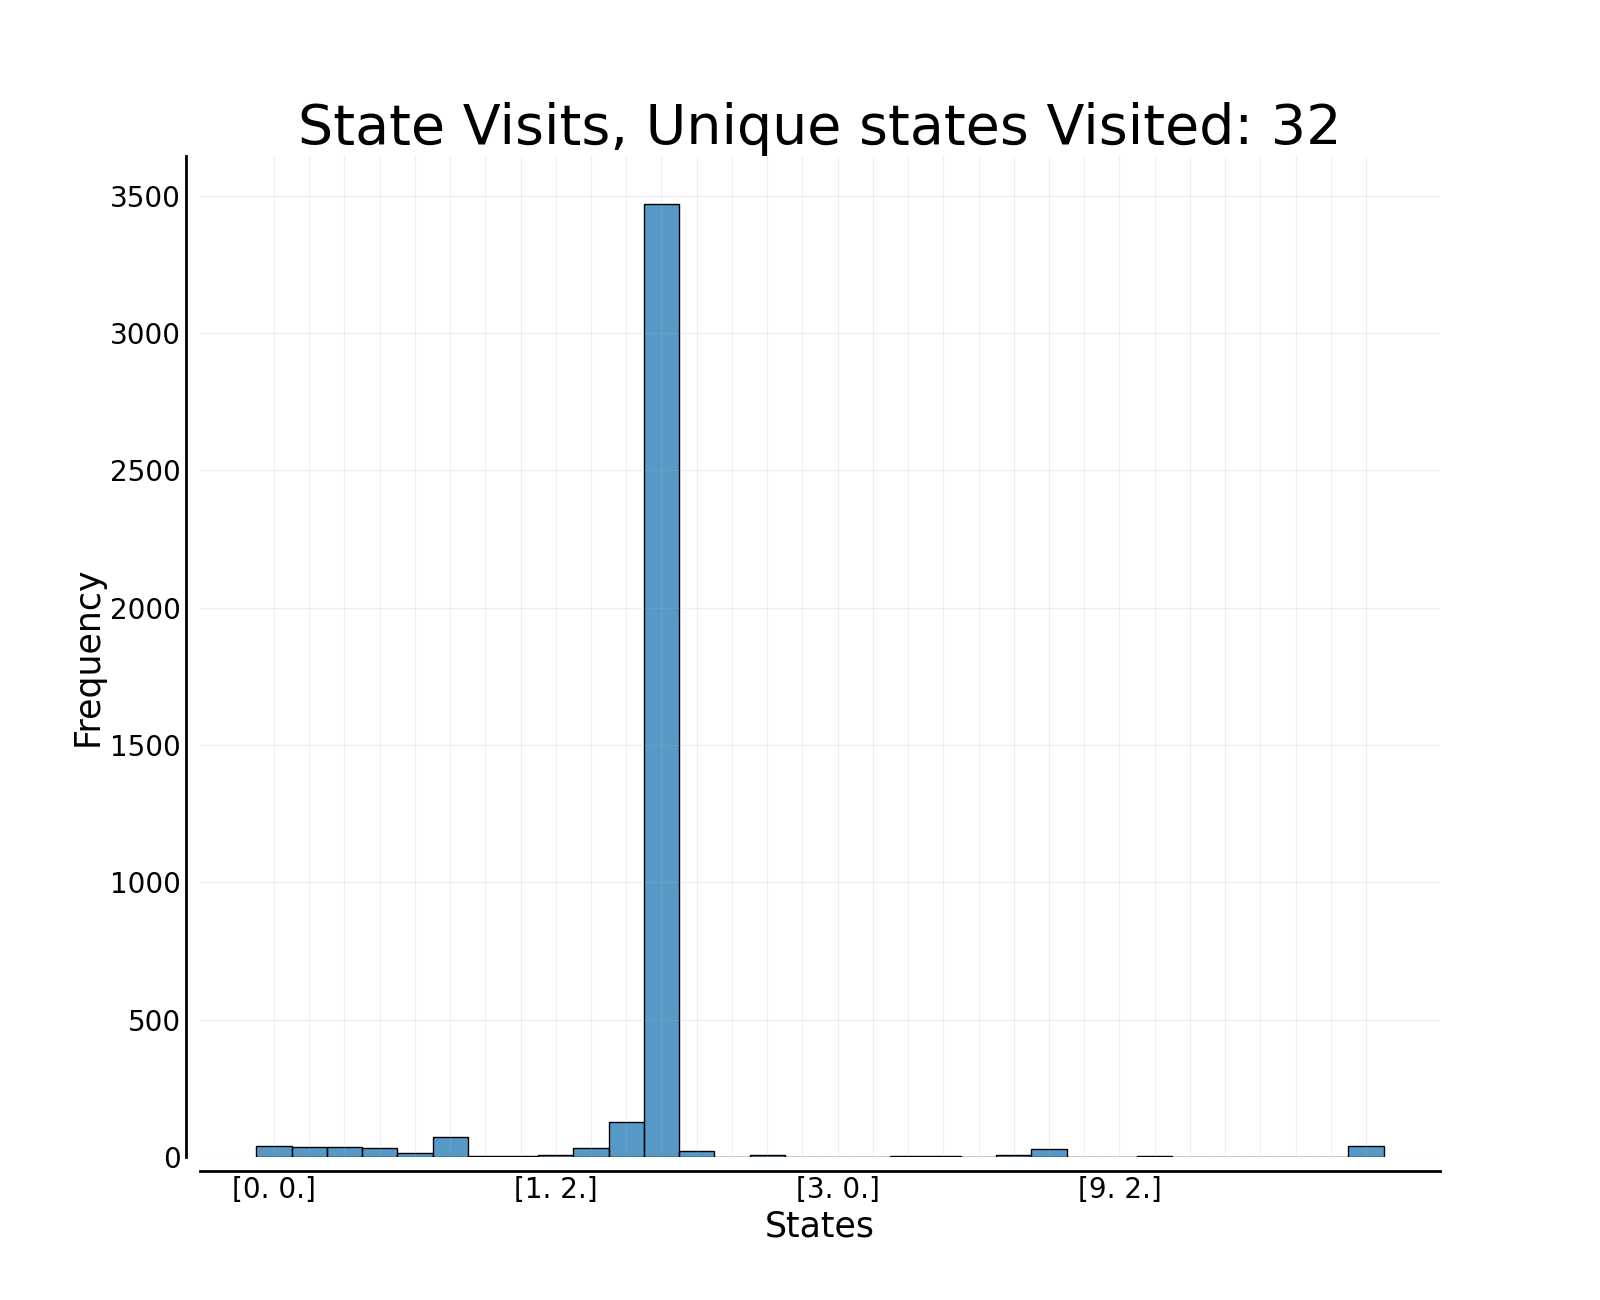
\includegraphics[width=0.31\linewidth]{figures/visualisation/state_action_coverage_RTG_7_5_1.png}
    }
    \hfill
    \subfigure[Goal Location (4,6)]{
        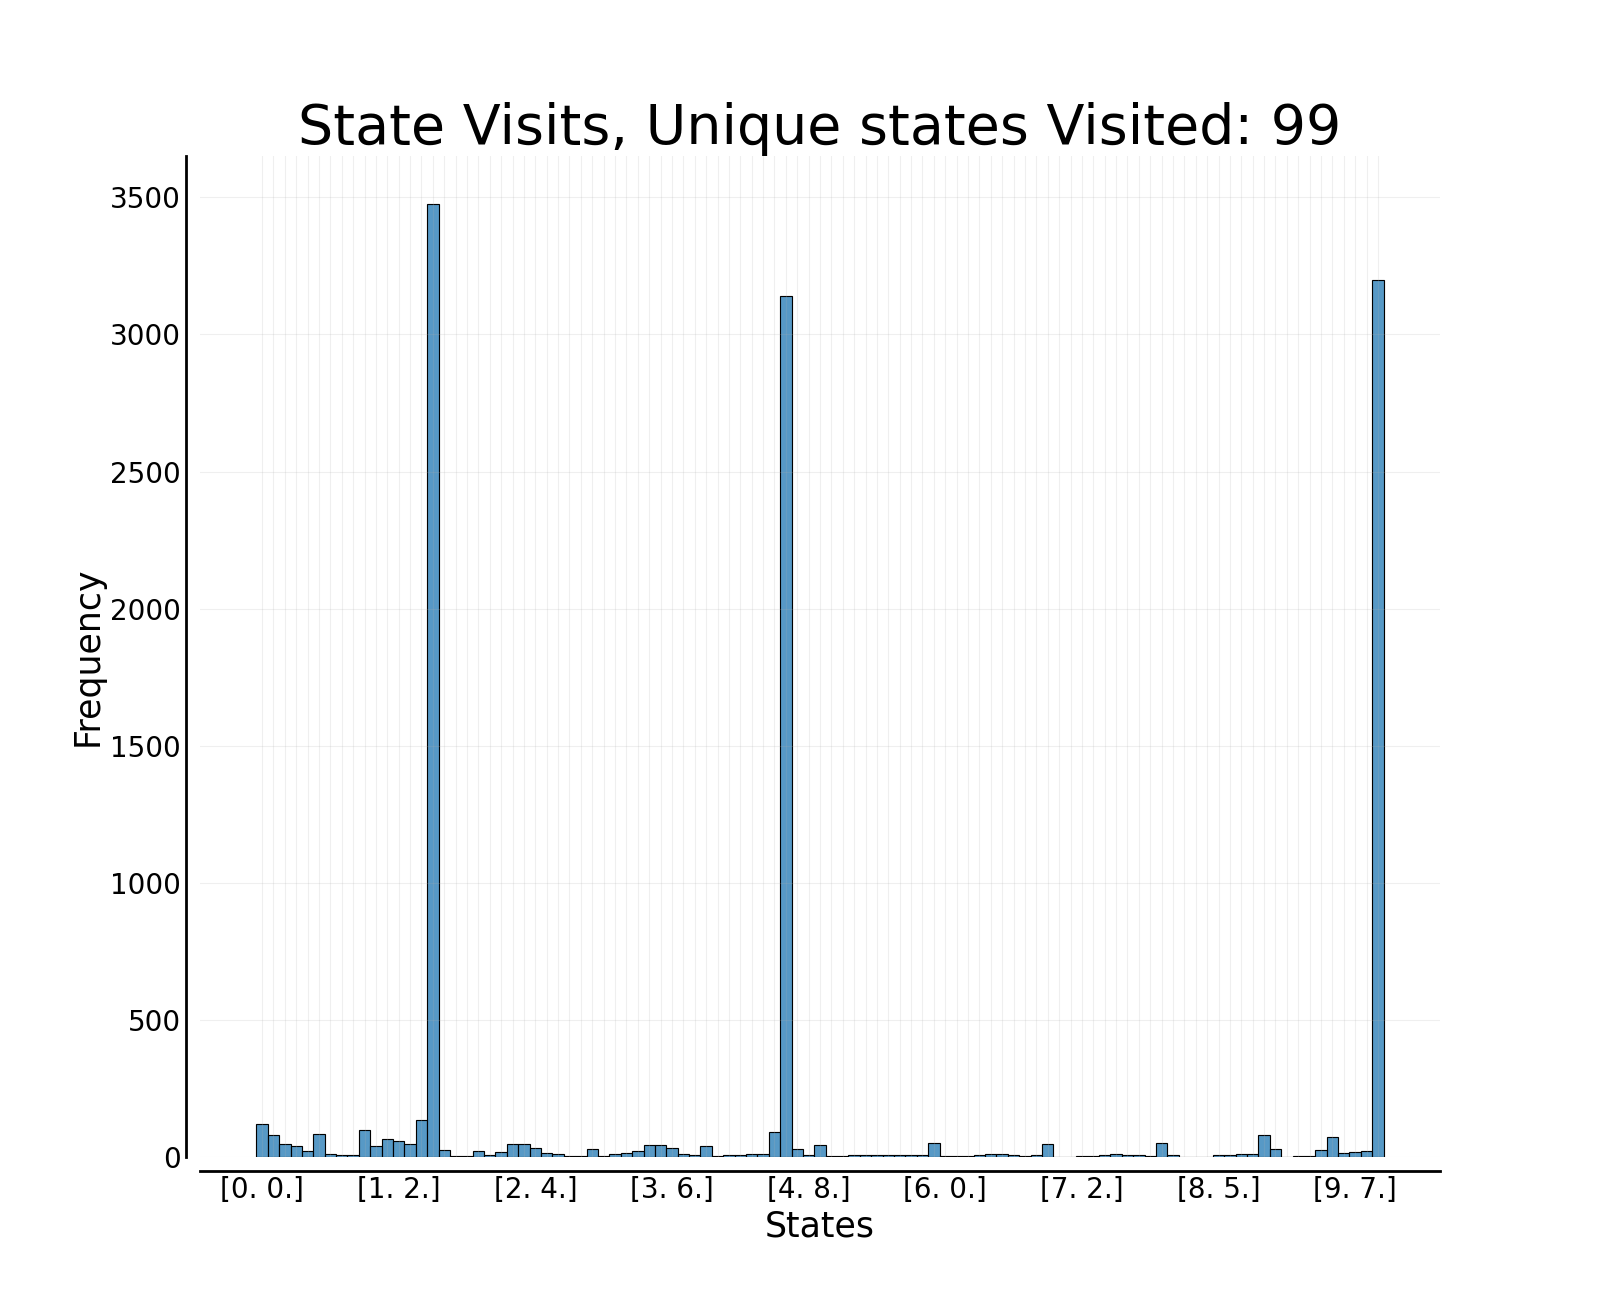
\includegraphics[width=0.31\linewidth]{figures/visualisation/state_action_coverage_RTG_0_6_4.png}
    }
    \caption{We count the state visitations on Dark-Room $10\times10$ over all ICL trials for three different goal locations: $(5,8)$, $(5,1)$, and $(4,6)$. The total number of states is 100. The agent attempts to visit all states at least once. Once the agent finds the goal, it starts exploiting (e.g., goal location $(5,1)$).}
    \label{appendix:exploration}
\end{figure*}

\textbf{Delusions in RA-DT.} 
Furthermore, we find that in some unsuccessful trials, the agent repeatedly performs the same suboptimal action sequences.  
\citet{Ortega:21} refer to such behaviour as delusions. 
In Figure \ref{appendix:delusions}, we illustrate two examples in which the agent suffers from delusions and does not recover until the end of the episode.

\begin{figure}[ht]
    \centering
    \subfigure[$(0,2) \rightarrow (0,4)$]{
        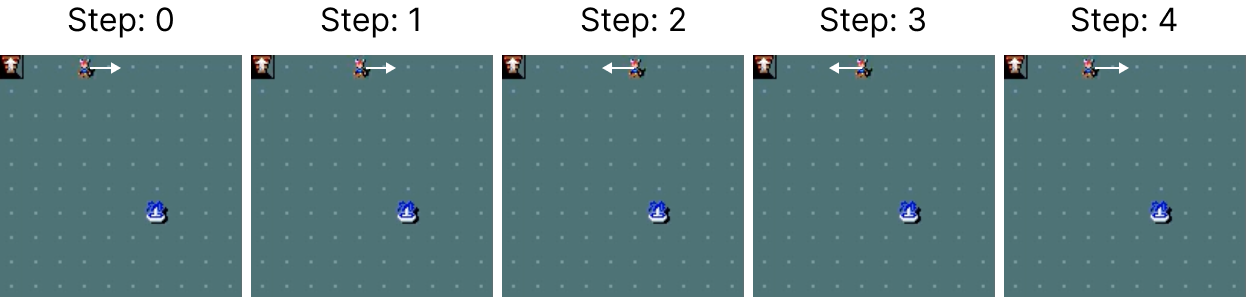
\includegraphics[width=1.0\linewidth]{figures/visualisation/delusions_1.png}  
    }
    \subfigure[$(3,9) \rightarrow (4,9)$]{
        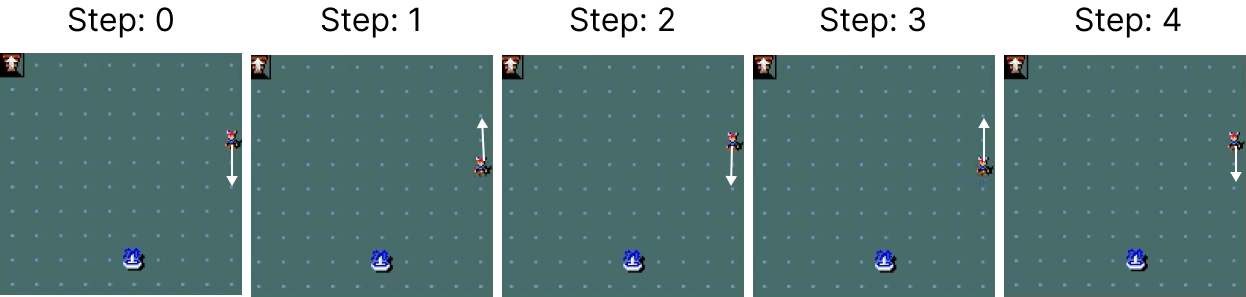
\includegraphics[width=1.0\linewidth]{figures/visualisation/delusions_2.png}  
    }
    \caption{Illustrations of delusions in RA-DT on Dark-Room $10\times10$. In \textbf{(a)}, the agent navigates from state (0, 2) to (0, 4) and returns to (0, 2). In \textbf{(b)}, the agent 
    The agent goes from state (3, 9) and (4, 9) and back. In both examples, the agent repeats the unsuccessful action sequence.}
    \label{appendix:delusions}
\end{figure}

\subsection{Maze-Runner}\label{appendix:expdetails-mazerunner}
In Figures \ref{fig:mazerunner-avg-bar} and \ref{fig:mazerunner-icl}, we report the average performances at the end of the training (100K) for both the 100 train and 20 evaluation mazes, as well as the corresponding ICL curves, respectively.

While RA-DT outperforms competitors, we observe a considerable performance gap between train mazes and test mazes (0.65 vs. 0.4 reward, see Figure \ref{fig:mazerunner-avg-bar}).
This indicates that RA-DT struggles to solve difficult, unseen mazes.
We believe that this gap is an artifact of the small pre-training distribution of 100 mazes and can be closed by increasing the number of pre-training mazes.
Furthermore, increasing the number of ICL trials may also enhance the performance. 
\begin{figure}[h]
    \centering
    
\includegraphics[width=0.75\linewidth]{figures/mazerunner/15x15/bar_legend.png}  
    
    \subfigure[100 Train Mazes]{
        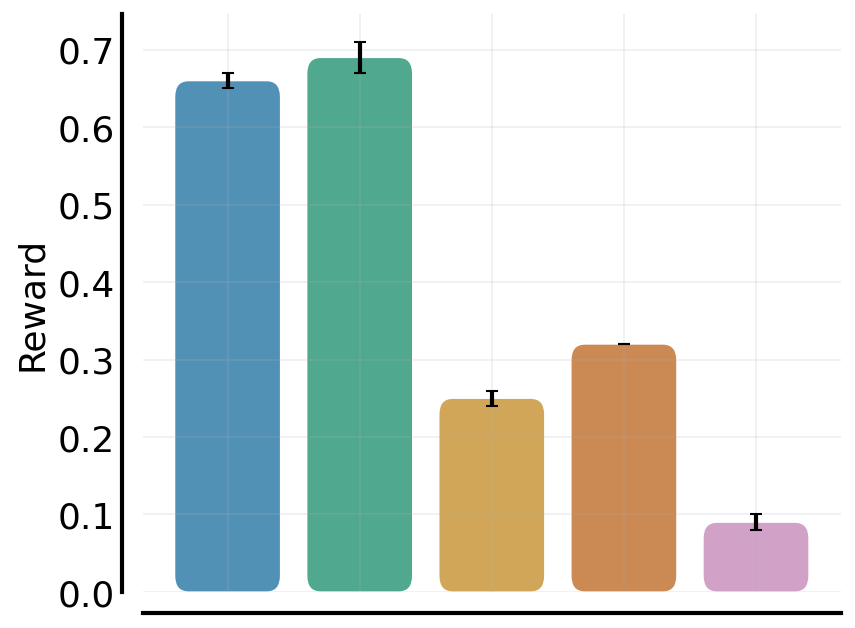
\includegraphics[width=0.31\linewidth]{figures/mazerunner/15x15/bar_train.png}
        \label{fig:X}
    }
    \hspace{1cm}
    \subfigure[20 Test Mazes]{
        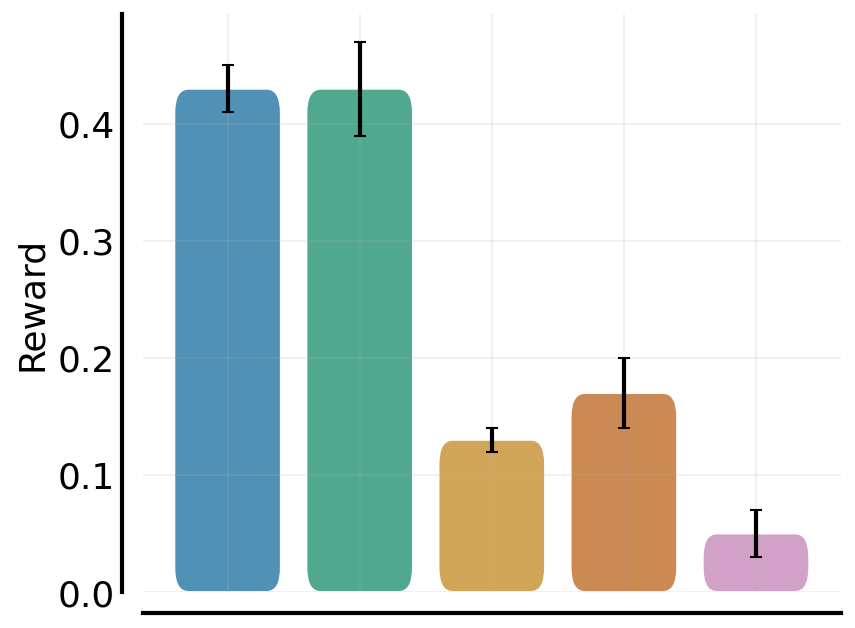
\includegraphics[width=0.31\linewidth]{figures/mazerunner/15x15/bar_eval.png}
        \label{fig:X}
    }
    \caption{Average performance on \textbf{(a)} 100 train and \textbf{(b)} 20 test mazes at end of training (100K steps). We evaluate each agent for 30 episodes and report the mean reward (+ 95\% CI) over 3 seeds.}
    \label{fig:mazerunner-avg-bar}
\end{figure}

\begin{figure}[h]
    \centering
    
\includegraphics[width=0.75\linewidth]{figures/mazerunner/15x15/legend.png}  
    
    \subfigure[100 Train Mazes]{
        
\includegraphics[width=0.31\linewidth]{figures/mazerunner/15x15/train_icl.png}
        \label{fig:X}
    }
    \hspace{1cm}
    \subfigure[20 Test Mazes]{
        
\includegraphics[width=0.31\linewidth]{figures/mazerunner/15x15/eval_icl.png}
        \label{fig:X}
    }
    \caption{ICL on \textbf{(a)} 100 train and \textbf{(b)} 20 test mazes at end of training (100K steps). We evaluate each agent for 30 episodes and report the mean reward (+ 95\% CI) over 3 seeds.}
    \label{fig:mazerunner-icl}
\end{figure}

\subsection{Meta-World}\label{appendix:expdetails-metaworld}
In Figures \ref{fig:ML45-avg} and \ref{fig:ML45-icl}, we show the training curves across the entire training period (200K steps), and the corresponding ICL curves at the end of training for both ML45 and ML5. 

Generally, we observe that RA-DT outperforms competitors on the evaluation tasks in terms of average performance. 
However, on the training task, the average performance of RA-DT is lower than that of vanilla DT.
AD and DPT lag behind both methods. 
One potential reason is the RTG conditioning, which biases DT and RA-DT towards higher quality behaviour. 

    

\begin{figure}[h]
    \centering
    
\includegraphics[width=0.5\linewidth]{figures/metaworld/legend.png}  
    
    \subfigure[ML45]{
        
\includegraphics[width=0.31\linewidth]{figures/metaworld/train.png}
        \label{fig:X}
    }
    \hspace{1cm}
    \subfigure[MT5]{
        
\includegraphics[width=0.31\linewidth]{figures/metaworld/eval.png}
        \label{fig:X}
    }
    \caption{Learning curves on \textbf{(a)} ML45 and \textbf{(b)} MT5 over the full training period (200K). We evaluate each agent for 30 episodes and report the mean reward (+ 95\% CI) over 3 seeds.}
    \label{fig:ML45-avg}
\end{figure}

Nevertheless, we do not observe improved ICL performance of RA-DT on evaluation tasks. 
While all in-context RL methods exhibit in-context improvement on the training tasks (ML45), neither RA-DT nor other methods show signs of improvement on the evaluation tasks (MT5).

\begin{figure}[h]
    \centering
    
\includegraphics[width=0.5\linewidth]{figures/metaworld/legend.png}  
    
    \subfigure[ML45]{
        
\includegraphics[width=0.31\linewidth]{figures/metaworld/train_icl.png}
        \label{fig:X}
    }
    \hspace{1cm}
    \subfigure[MT5]{
        
\includegraphics[width=0.31\linewidth]{figures/metaworld/eval_icl.png}
        \label{fig:X}
    }
    \caption{ICL performance on \textbf{(a)} ML45 and \textbf{(b)} MT5 at end of training (200K steps). We evaluate each agent for 30 episodes and report the mean reward (+ 95\% CI) over 3 seeds.}
    \label{fig:ML45-icl}
\end{figure}

In addition, we provide the average rewards and data-normalized scores for the MT5 evaluation tasks in Table \ref{tab:metaworld-eval}.

\begin{table}[h]
    \centering
    \caption{Meta-World Evaluation Tasks.}
\begin{tabular}{lcccc}
    \toprule
    \textbf{Environment} &  \textbf{DT} & \textbf{AD} & \textbf{DPT} & \textbf{RA-DT} \\
    \midrule
    \multicolumn{5}{c}{\textbf{Reward}} \\
bin-picking        &           62.28 ± 34.37 &          42.63 ± 17.47 &           27.52 ± 14.07 &          14.47 ± 1.79 \\
box-close          &            70.34 ± 6.72 &           85.4 ± 14.96 &           106.79 ± 23.7 &        110.09 ± 46.69 \\
hand-insert        &             27.38 ± 3.1 &          51.82 ± 59.93 &            13.06 ± 0.15 &        182.25 ± 99.63 \\
door-lock          &           229.76 ± 11.4 &        333.89 ± 161.77 &           239.2 ± 20.19 &         219.44 ± 2.51 \\
door-unlock        &         588.66 ± 454.89 &          450.71 ± 8.37 &          249.17 ± 63.38 &       1163.02 ± 36.42 \\
\textbf{Average}                            &          195.68 ± 97.31 &         192.89 ± 23.48 &          127.15 ± 16.97 &        337.85 ± 34.94 \\
\midrule
\multicolumn{5}{c}{\textbf{Data-normalized Scores}} \\
bin-picking &             0.24 ± 0.14 &            0.16 ± 0.07 &             0.09 ± 0.06 &           0.04 ± 0.01 \\
box-close   &            -0.07 ± 0.01 &           -0.03 ± 0.03 &             0.01 ± 0.05 &            0.02 ± 0.1 \\
hand-insert &              0.02 ± 0.0 &            0.04 ± 0.05 &              0.01 ± 0.0 &           0.15 ± 0.08 \\
door-lock   &              0.0 ± 0.01 &            0.08 ± 0.12 &             0.01 ± 0.01 &            -0.0 ± 0.0 \\
door-unlock &             0.27 ± 0.31 &            0.18 ± 0.01 &             0.04 ± 0.04 &           0.66 ± 0.02 \\
\textbf{Average}                              &             0.09 ± 0.08 &            0.08 ± 0.01 &             0.03 ± 0.03 &           0.17 ± 0.04 \\
\bottomrule
\end{tabular}
\label{tab:metaworld-eval}
\end{table}


\subsection{DMControl}\label{appendix:expdetails-dmc}
In Figures \ref{fig:dmc-avg} and \ref{fig:dmc-icl}, we show the training curves across the entire training period (200K steps) and the corresponding ICL curves at the end of training for both DMC11 and DMC5. 

Similar to our results on Meta-World, we observe that RA-DT outperforms competitors on average. 
However, we do not observe in-context improvement on the evaluation tasks. 
    

\begin{figure}[h]
    \centering
    
\includegraphics[width=0.75\linewidth]{figures/dmcontrol/legend_new.png}  
    
    \subfigure[DMC11]{
        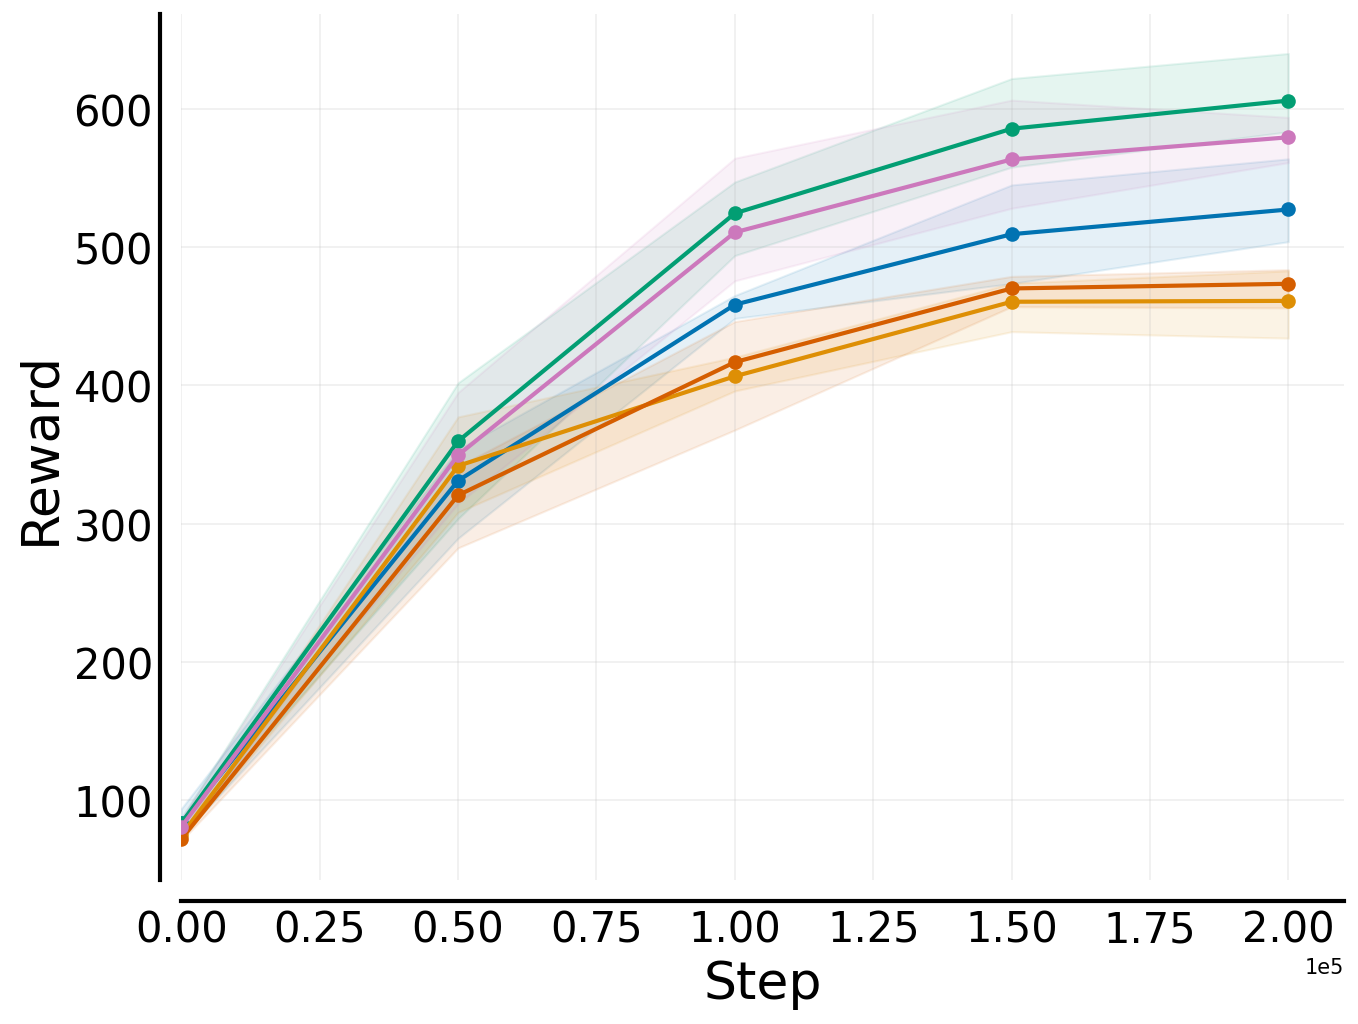
\includegraphics[width=0.31\linewidth]{figures/dmcontrol/train_new.png}
        \label{fig:X}
    }
    \hspace{1cm}
    \subfigure[DMC5]{
        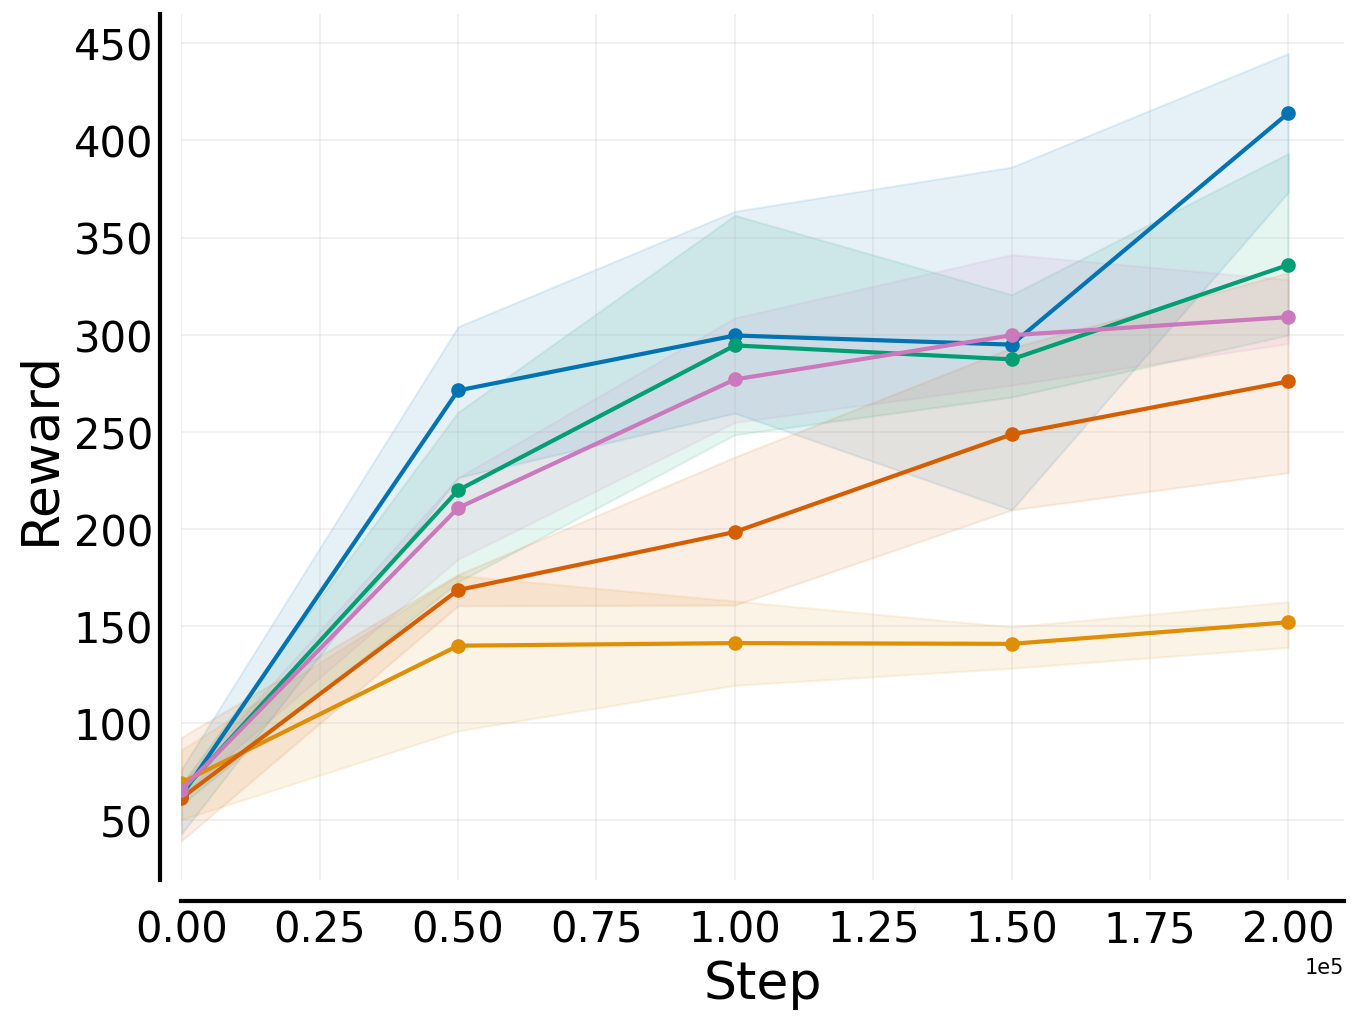
\includegraphics[width=0.31\linewidth]{figures/dmcontrol/eval_new.png}
        \label{fig:X}
    }
    \caption{Average performance on \textbf{(a)} DMC11 and \textbf{(b)} DMC5 at end of training (200K steps). We evaluate each agent for 30 episodes and report the mean reward (+ 95\% CI) over 3 seeds.}
    \label{fig:dmc-avg}
\end{figure}

\begin{figure}[h]
    \centering
    
\includegraphics[width=0.75\linewidth]{figures/dmcontrol/legend_new.png}  
    
    \subfigure[DMC11]{
        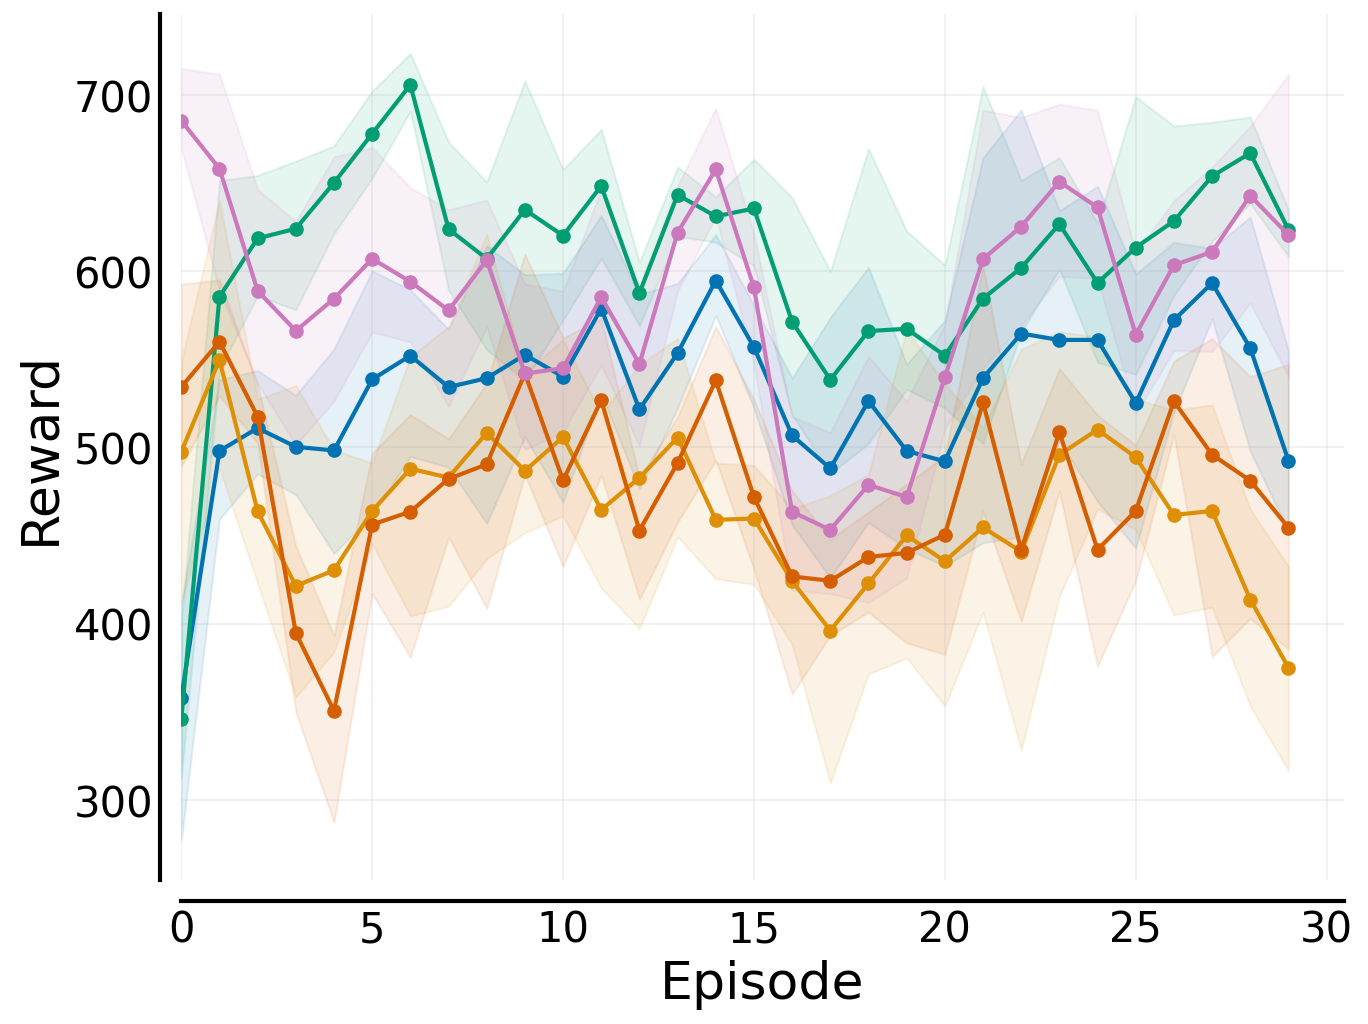
\includegraphics[width=0.31\linewidth]{figures/dmcontrol/train_icl_new.png}
        \label{fig:x}
    }
    \hspace{1cm}
    \subfigure[DMC5]{
        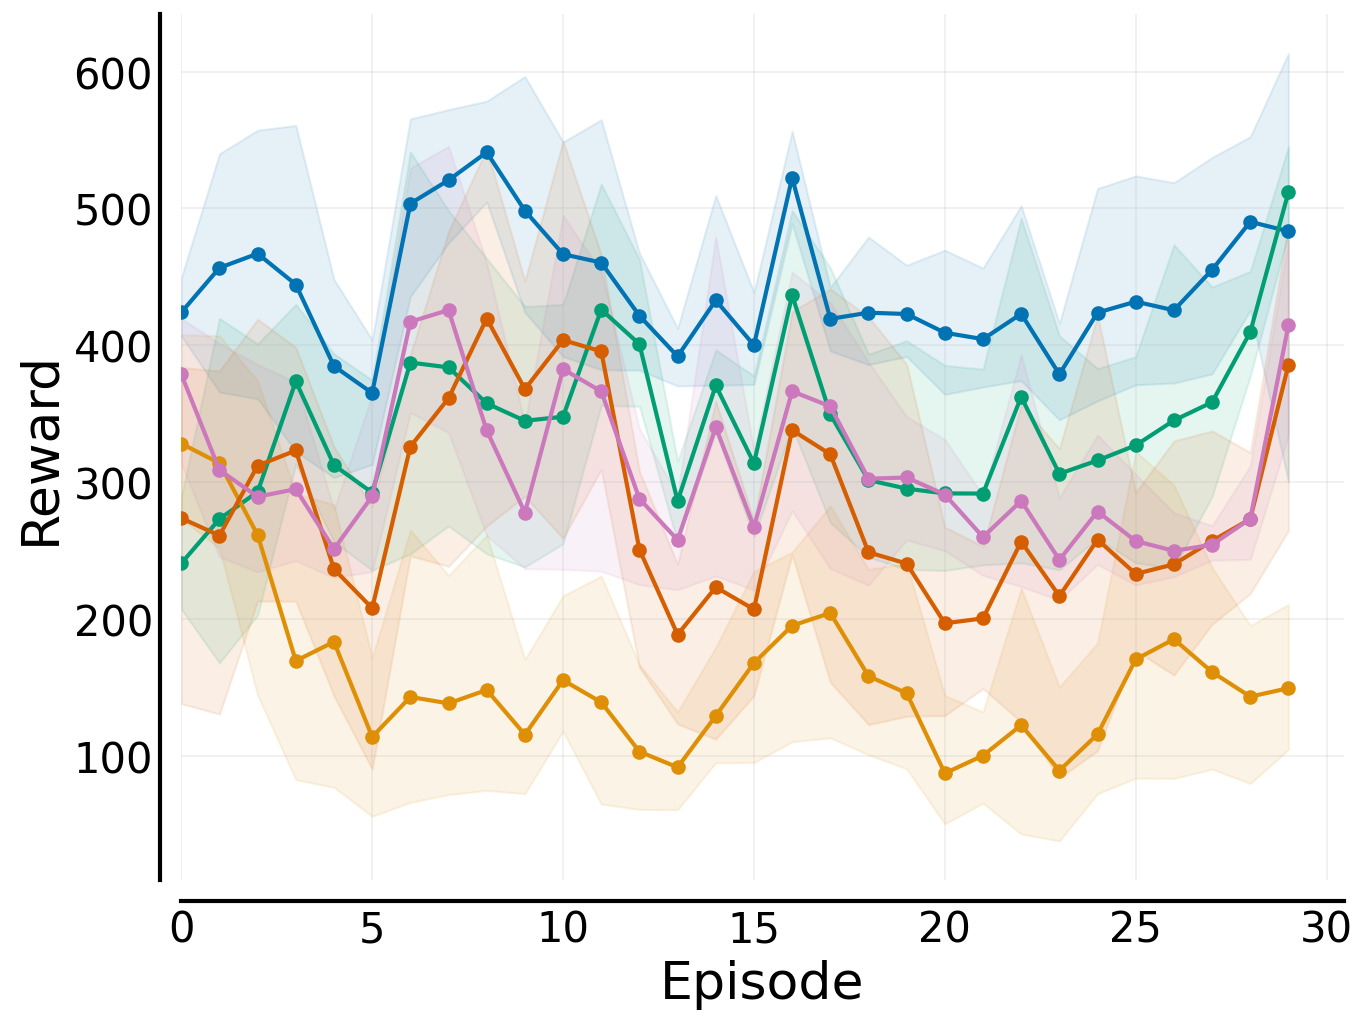
\includegraphics[width=0.31\linewidth]{figures/dmcontrol/eval_icl_new.png}
        \label{fig:X}
    }
    \caption{ICL performance on \textbf{(a)} DMC11 and \textbf{(b)} DMC5 at end of training (200K steps). We evaluate each agent for 30 episodes and report the mean reward (+ 95\% CI) over 3 seeds.}
    \label{fig:dmc-icl}
\end{figure}\

In addition, we show the average rewards obtained and corresponding data-normalized scores for all DMC5 evaluation tasks in Table \ref{tab:dmcontrol-eval}.

\begin{table}[h]
    \centering
    \caption{DMControl Eval Tasks.}
\begin{tabular}{lcccc}
    \toprule
    \textbf{Environment}                    &  \textbf{AD}        & \textbf{DT} & \textbf{DPT} & \textbf{RA-DT} \\
    \midrule
    \multicolumn{5}{c}{\textbf{Reward}} \\
    cartpole-balance                                             & 211.96 $\pm$ 62.8   & 946.49 $\pm$ 44.91  & 703.89 $\pm$ 263.11 & 910.1 $\pm$ 106.0    \\
    finger-turn\_hard                                            & 199.34 $\pm$ 46.0   & 253.13 $\pm$ 43.0   & 295.2 $\pm$ 51.88   & 336.37 $\pm$ 16.51  \\
    pendulum-swingup                                             & 1.18 $\pm$ 2.04     & 0.0 $\pm$ 0.0       & 0.0 $\pm$ 0.0       & 0.0 $\pm$ 0.0       \\
    reacher-hard                                                 & 34.22 $\pm$ 17.25   & 167.7 $\pm$ 42.86  & 157.29 $\pm$ 94.79 & 95.4 $\pm$ 15.4    \\
    walker-walk                                                  & 326.42 $\pm$ 102.52 & 189.46 $\pm$ 10.22  & 257.11 $\pm$ 57.21  & 877.9 $\pm$ 15.2    \\
    \textbf{Average}                                             &         154.63 $\pm$ 12.17 &        311.36 $\pm$ 12.49 &        282.7 $\pm$ 54.62 &       443.95 $\pm$ 25.7 \\
    \midrule
    \multicolumn{5}{c}{\textbf{Data-normalized Score}} \\
    cartpole-balance                                             & -0.24 $\pm$ 0.11  & 1.01 $\pm$ 0.08   & 0.6 $\pm$ 0.45   & 0.95 $\pm$ 0.18   \\
    finger-turn\_hard                                            & 0.25 $\pm$ 0.07   & 0.33 $\pm$ 0.07   & 0.4 $\pm$ 0.08   & 0.47 $\pm$ 0.03   \\
    pendulum-swingup                                             & 0.0 $\pm$ 0.0     & 0.0 $\pm$ 0.0     & 0.0 $\pm$ 0.0     & 0.0 $\pm$ 0.0     \\
    reacher-hard                                                 & 0.03 $\pm$ 0.02   & 0.21 $\pm$ 0.06   & 0.19 $\pm$ 0.12  & 0.11 $\pm$ 0.02   \\
    walker-walk                                                  & 0.4 $\pm$ 0.14    & 0.21 $\pm$ 0.01   & 0.31 $\pm$ 0.08   & 1.14 $\pm$ 0.02   \\
    \textbf{Average}    &   0.09 $\pm$ 0.02 &           0.35 $\pm$ 0.02 &    0.3 $\pm$ 0.09   &   0.53 $\pm$ 0.04 \\
    \bottomrule
    \end{tabular}
    \label{tab:dmcontrol-eval}
\end{table}


\subsection{Procgen}\label{appendix:expdetails-procgen}
In Figures \ref{fig:procgen-avg} and \ref{fig:procgen-avg-icl}, we show the training curves across the entire training period (200K steps), and the corresponding ICL curves at the end of training for PG12-Seen, PG12-Unseen, and PG4.
While we observe slightly better average performance of RA-DT compared to competitors, we do not find any in-context improvement. 

\textbf{RA-DT constructs bursty sequences.}. 
Building on work by \citet{Chan:22}, \citet{Raparthy:23} identified trajectory burstiness as one important property for ICL to emerge on the Procgen benchmark.
A given sequence is considered bursty if it contains at least two trajectories from the same seed (or level).
Consequently, the agent obtains relevant information that it can leverage to predict the next action. 
Therefore, we follow \citet{Raparthy:23} and always provide a trajectory from the same seed in the context of AD and DPT. 
Indeed, we observed that this improves performance, compared to not taking trajectory burstiness into account.
Interestingly, we found that RA-DT retrieves trajectories from the same or similar seeds (seed accuracy of $~80$\% %
This intuitively makes sense, as retrieval directly searches for the most relevant experiences (see Section \ref{sec:reweighting}). 
Therefore, for RA-DT, we do not provide additional information that indicates with which environment the trajectory was generated. 

\begin{figure}[h]
    \centering
    
\includegraphics[width=0.5\linewidth]{figures/procgen/legend.png}  
    
    \subfigure[PG12-Seen]{
        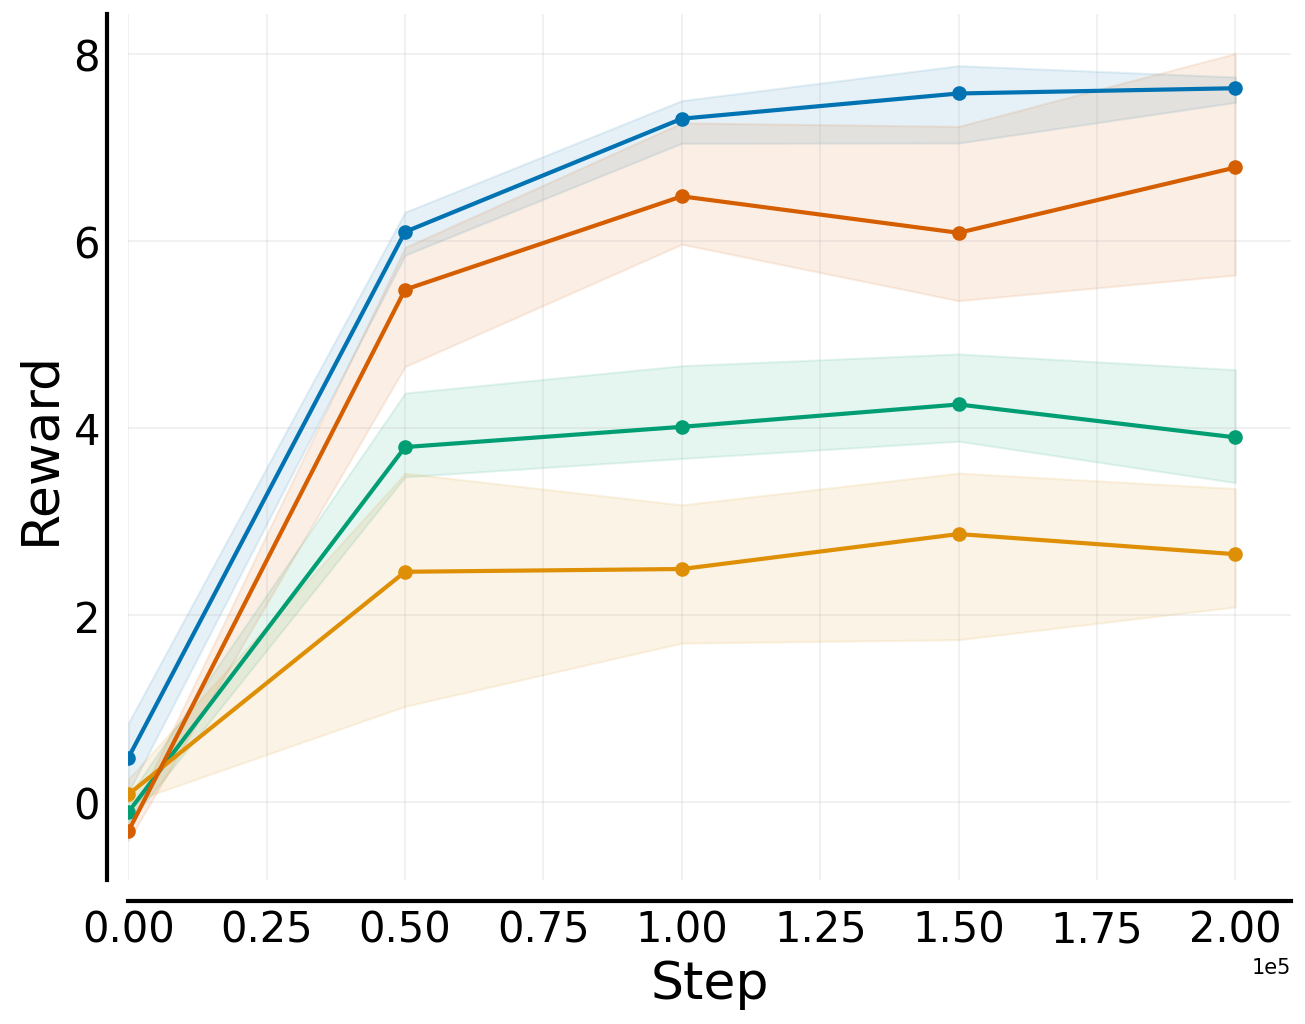
\includegraphics[width=0.31\linewidth]{figures/procgen/train_seeds.png}
        \label{fig:X}
    }
    \hfill
    \subfigure[PG12-Unseen]{
        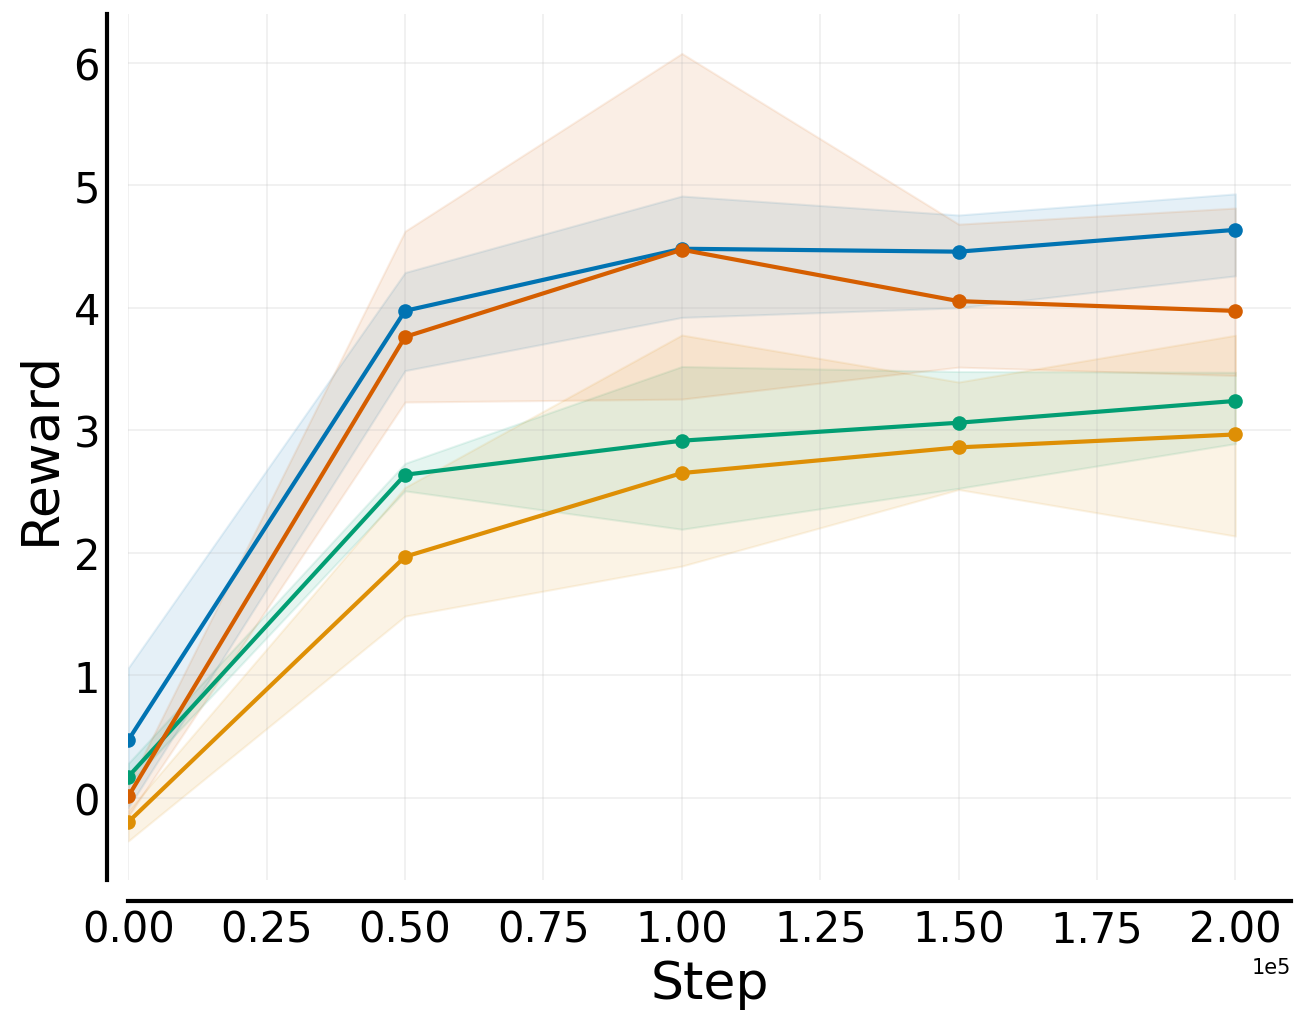
\includegraphics[width=0.31\linewidth]{figures/procgen/train_eval_seeds.png}
        \label{fig:X}
    }
    \hfill
    \subfigure[PG4]{
        
\includegraphics[width=0.31\linewidth]{figures/procgen/eval.png}
        \label{fig:X}
    }
    \caption{Learning curves on Procgen across \textbf{(a)} PG12-Seen, \textbf{(b)} PG12-Unseen, and \textbf{(c)} PG4 seed over the full training period. We train for 200K steps, evaluate every 50K steps for 30 episodes, and report mean reward (+ 95\% CI) over 3 seeds.}
    \label{fig:procgen-avg}
\end{figure}

\begin{figure}[h]
    \centering
    
\includegraphics[width=0.5\linewidth]{figures/procgen/legend.png}  
    
    \subfigure[PG12-Seen]{
        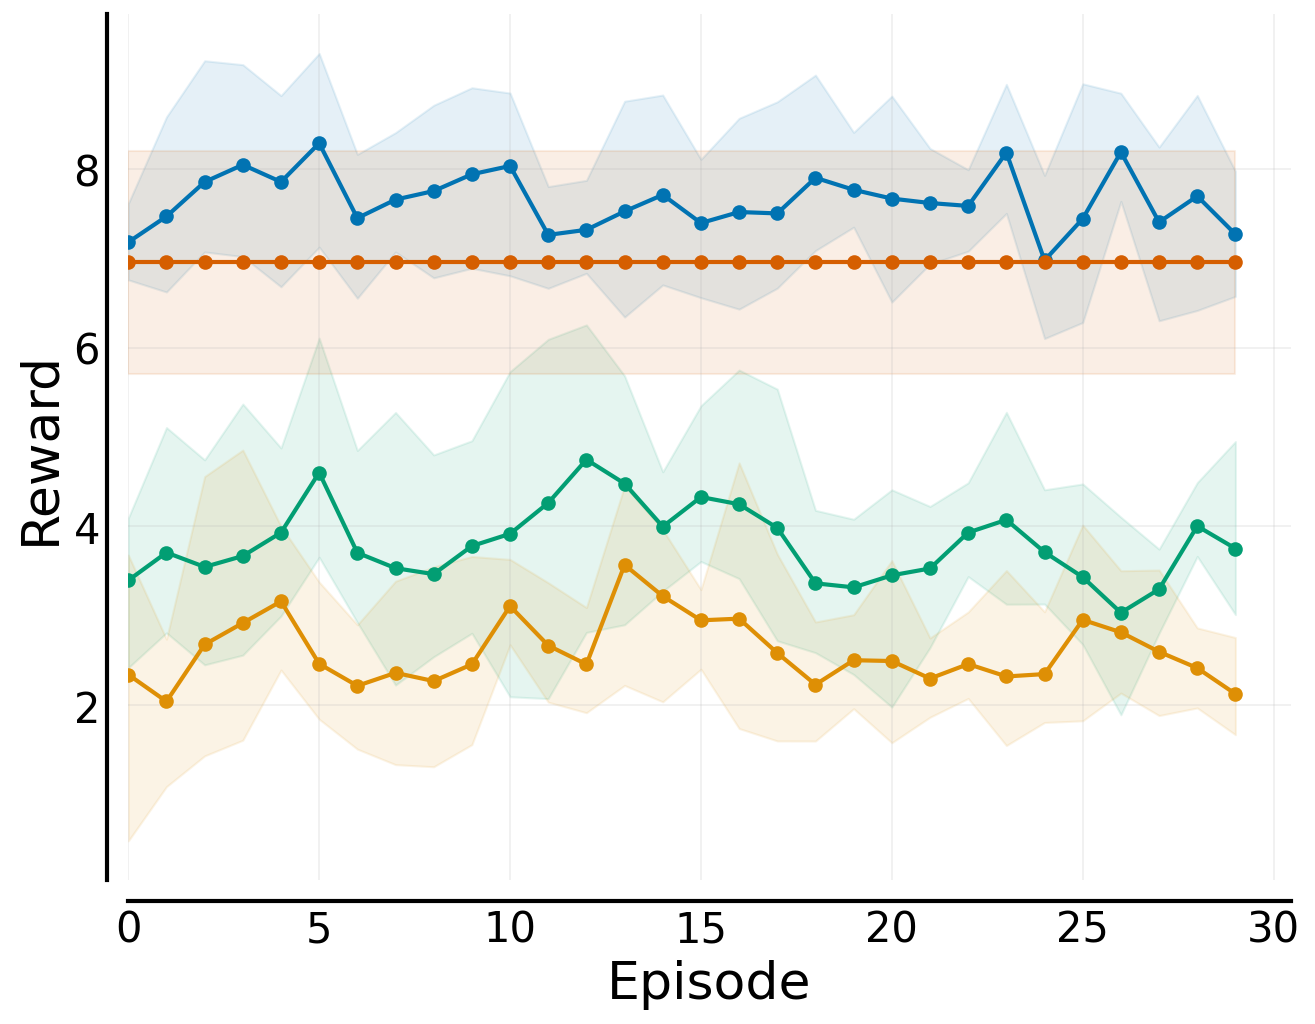
\includegraphics[width=0.31\linewidth]{figures/procgen/train_seeds_icl.png}
        \label{fig:X}
    }
    \hfill
    \subfigure[PG12-Unseen]{
        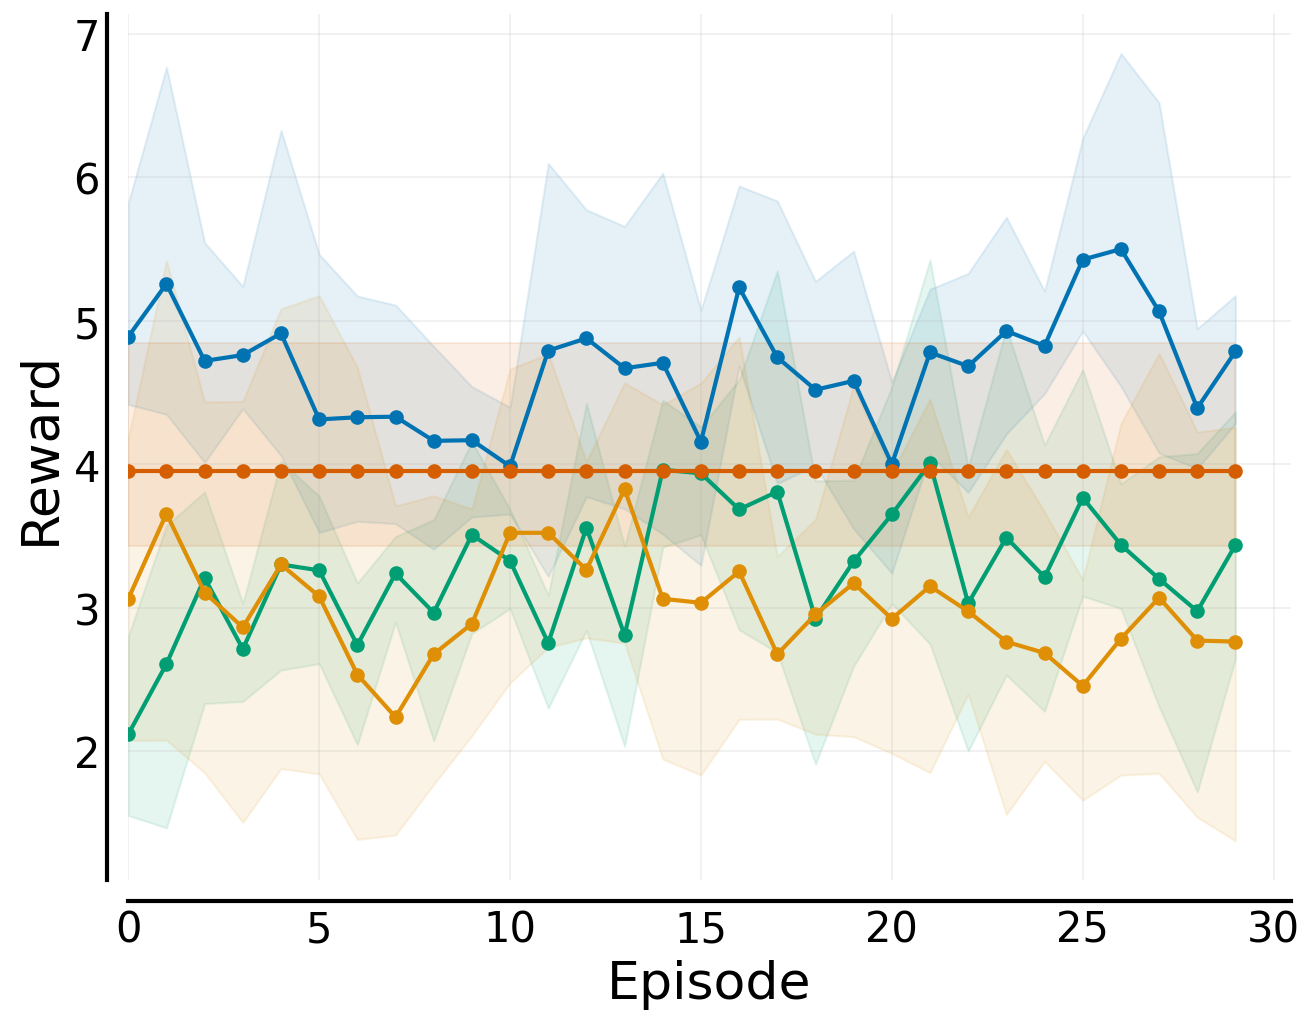
\includegraphics[width=0.31\linewidth]{figures/procgen/train_eval_seeds_icl.png}
        \label{fig:X}
    }
    \hfill
    \subfigure[PG4]{
        
\includegraphics[width=0.31\linewidth]{figures/procgen/eval_icl.png}
        \label{fig:X}
    }
    \caption{ICL performances on Procgen across \textbf{(a)} PG12-Seen, \textbf{(b)} PG12-Unseen, and \textbf{(c)} PG4. We evaluate for 30 episodes, and report mean reward (+ 95\% CI) over 3 seeds.}
    \label{fig:procgen-avg-icl}
\end{figure}

\begin{table}[h]
    \centering
    \caption{Procgen Train Tasks, Train Seeds.}
    \begin{tabular}{@{} l c c c c@{}}
    \toprule
    \textbf{Environment} & \textbf{DT} & \textbf{AD} & \textbf{DPT} & \textbf{RA-DT} \\ \midrule
    \multicolumn{5}{c}{\textbf{Rewards}} \\ 
    \texttt{bigfish}     &                  4.67 $\pm$ 3.51 &                    2.0 $\pm$ 0.76 &                    2.41 $\pm$ 0.1 &            5.21 $\pm$ 0.25 \\
    \texttt{bossfight}   &                    1.0 $\pm$ 0.0 &                   0.46 $\pm$ 0.55 &                    0.9 $\pm$ 0.26 &            1.31 $\pm$ 0.08 \\
    \texttt{caveflyer}   &                  3.33 $\pm$ 5.77 &                   0.22 $\pm$ 0.19 &                    3.0 $\pm$ 3.28 &             9.67 $\pm$ 0.0 \\
    \texttt{chaser}      &                  1.49 $\pm$ 1.05 &                    1.7 $\pm$ 0.49 &                   1.64 $\pm$ 0.59 &            2.78 $\pm$ 0.46 \\
    \texttt{coinrun}     &                  6.67 $\pm$ 5.77 &                   5.89 $\pm$ 0.69 &                   7.78 $\pm$ 1.17 &            8.33 $\pm$ 0.33 \\
    \texttt{dodgeball}   &                  7.33 $\pm$ 7.57 &                   2.47 $\pm$ 0.79 &                    2.8 $\pm$ 1.44 &            8.98 $\pm$ 0.87 \\
    \texttt{fruitbot}    &                   8.0 $\pm$ 2.65 &                   7.66 $\pm$ 0.62 &                   7.19 $\pm$ 1.09 &             8.6 $\pm$ 0.23 \\
    \texttt{heist}       &                   10.0 $\pm$ 0.0 &                     0.0 $\pm$ 0.0 &                   0.33 $\pm$ 0.58 &            9.11 $\pm$ 1.02 \\
    \texttt{leaper}      &                    0.0 $\pm$ 0.0 &                     0.0 $\pm$ 0.0 &                     0.0 $\pm$ 0.0 &              0.0 $\pm$ 0.0 \\
    \texttt{maze}        &                   10.0 $\pm$ 0.0 &                   0.11 $\pm$ 0.19 &                   5.56 $\pm$ 5.09 &            8.56 $\pm$ 0.69 \\
    \texttt{miner}      &                   13.0 $\pm$ 0.0 &                   0.94 $\pm$ 0.48 &                   1.23 $\pm$ 1.15 &           11.37 $\pm$ 0.23 \\
    \texttt{starpilot}  &                 18.0 $\pm$ 10.54 &                   9.72 $\pm$ 4.78 &                   12.9 $\pm$ 4.69 &           17.82 $\pm$ 0.72 \\
    \textbf{Avgerage} &                  6.96 $\pm$ 1.25 &                    2.6 $\pm$ 0.62 &                   3.81 $\pm$ 0.68 &            7.64 $\pm$ 0.07 \\
    \midrule
    \multicolumn{5}{c}{\textbf{Human-normalized scores}} \\ 
    \texttt{bigfish}             &                  0.09 $\pm$ 0.09 &                   0.03 $\pm$ 0.02 &                    0.04 $\pm$ 0.0 &            0.11 $\pm$ 0.01 \\
    \texttt{bossfight}           &                   0.04 $\pm$ 0.0 &                   -0.0 $\pm$ 0.04 &                   0.03 $\pm$ 0.02 &            0.06 $\pm$ 0.01 \\
    \texttt{caveflyer}           &                 -0.02 $\pm$ 0.68 &                  -0.39 $\pm$ 0.02 &                  -0.06 $\pm$ 0.39 &             0.73 $\pm$ 0.0 \\
    \texttt{chaser}              &                  0.08 $\pm$ 0.08 &                    0.1 $\pm$ 0.04 &                   0.09 $\pm$ 0.05 &            0.18 $\pm$ 0.04 \\
    \texttt{coinrun}             &                  0.33 $\pm$ 1.15 &                   0.18 $\pm$ 0.14 &                   0.56 $\pm$ 0.23 &            0.67 $\pm$ 0.07 \\
    \texttt{dodgeball}           &                  0.33 $\pm$ 0.43 &                   0.06 $\pm$ 0.04 &                   0.07 $\pm$ 0.08 &            0.43 $\pm$ 0.05 \\
    \texttt{fruitbot}            &                  0.28 $\pm$ 0.08 &                   0.27 $\pm$ 0.02 &                   0.26 $\pm$ 0.03 &             0.3 $\pm$ 0.01 \\
    \texttt{heist}               &                    1.0 $\pm$ 0.0 &                   -0.54 $\pm$ 0.0 &                  -0.49 $\pm$ 0.09 &            0.86 $\pm$ 0.16 \\
    \texttt{leaper}              &                  -0.43 $\pm$ 0.0 &                   -0.43 $\pm$ 0.0 &                   -0.43 $\pm$ 0.0 &            -0.43 $\pm$ 0.0 \\
    \texttt{maze}                &                    1.0 $\pm$ 0.0 &                  -0.98 $\pm$ 0.04 &                   0.11 $\pm$ 1.02 &            0.71 $\pm$ 0.14 \\
    \texttt{miner}              &                    1.0 $\pm$ 0.0 &                  -0.05 $\pm$ 0.04 &                   -0.02 $\pm$ 0.1 &            0.86 $\pm$ 0.02 \\
    \texttt{starpilot}          &                  0.25 $\pm$ 0.17 &                   0.12 $\pm$ 0.08 &                   0.17 $\pm$ 0.08 &            0.25 $\pm$ 0.01 \\
    \textbf{Average}           &                       0.33 $\pm$ 0.14 &                  -0.14 $\pm$ 0.03 &                   0.03 $\pm$ 0.05 &             0.39 $\pm$ 0.0 \\
    \bottomrule
\end{tabular}
\label{tab:procgen-train-train}
\end{table}

\begin{table}[h]
    \centering
    \caption{Procgen Train Tasks, Evaluation Seeds.}
    \begin{tabular}{@{} l c c c c@{}}
    \toprule
    \textbf{Environment} & \textbf{DT} & \textbf{AD} & \textbf{DPT} & \textbf{RA-DT} \\ \midrule
    \multicolumn{5}{c}{\textbf{Rewards}} \\ 
    \texttt{bigfish}    &                    0.0 $\pm$ 0.0 &                   0.37 $\pm$ 0.64 &                   0.04 $\pm$ 0.08 &              0.38 $\pm$ 0.3 \\
    \texttt{bossfight}  &                  0.33 $\pm$ 0.58 &                   0.02 $\pm$ 0.02 &                   0.01 $\pm$ 0.02 &             0.02 $\pm$ 0.04 \\
    \texttt{caveflyer}  &                  6.67 $\pm$ 5.77 &                   3.67 $\pm$ 2.08 &                   7.67 $\pm$ 1.33 &             9.89 $\pm$ 0.19 \\
    \texttt{chaser}     &                  2.79 $\pm$ 0.65 &                    2.1 $\pm$ 0.67 &                   2.75 $\pm$ 0.93 &             5.17 $\pm$ 0.58 \\
    \texttt{coinrun}    &                   10.0 $\pm$ 0.0 &                   9.11 $\pm$ 0.84 &                   9.89 $\pm$ 0.19 &              10.0 $\pm$ 0.0 \\
    \texttt{dodgeball}  &                    0.0 $\pm$ 0.0 &                    0.29 $\pm$ 0.3 &                     0.0 $\pm$ 0.0 &             0.47 $\pm$ 0.41 \\
    \texttt{fruitbot}   &                    5.0 $\pm$ 4.0 &                   0.63 $\pm$ 1.65 &                   1.04 $\pm$ 0.83 &             4.01 $\pm$ 1.83 \\
    \texttt{heist}      &                    0.0 $\pm$ 0.0 &                     0.0 $\pm$ 0.0 &                     0.0 $\pm$ 0.0 &             0.11 $\pm$ 0.19 \\
    \texttt{leaper}     &                    0.0 $\pm$ 0.0 &                   0.11 $\pm$ 0.19 &                   0.11 $\pm$ 0.19 &             0.22 $\pm$ 0.38 \\
    \texttt{maze}       &                  6.67 $\pm$ 5.77 &                   2.78 $\pm$ 4.23 &                   1.67 $\pm$ 2.89 &              8.0 $\pm$ 3.46 \\
    \texttt{miner}     &                    0.0 $\pm$ 0.0 &                   0.58 $\pm$ 0.31 &                   0.41 $\pm$ 0.07 &             0.77 $\pm$ 0.09 \\
    \texttt{starpilot} &                   16.0 $\pm$ 1.0 &                   16.26 $\pm$ 5.4 &                  15.81 $\pm$ 3.27 &            17.12 $\pm$ 1.58 \\
    \textbf{Average}              &                  3.95 $\pm$ 0.78 &                   2.99 $\pm$ 0.92 &                   3.28 $\pm$ 0.26 &             4.68 $\pm$ 0.33 \\
    \midrule
    \multicolumn{5}{c}{\textbf{Human-normalized scores}} \\ 
    \texttt{bigfish}            &                  -0.03 $\pm$ 0.0 &                  -0.02 $\pm$ 0.02 &                   -0.02 $\pm$ 0.0 &            -0.02 $\pm$ 0.01 \\
    \texttt{bossfight}          &                 -0.01 $\pm$ 0.05 &                   -0.04 $\pm$ 0.0 &                   -0.04 $\pm$ 0.0 &             -0.04 $\pm$ 0.0 \\
    \texttt{caveflyer}          &                  0.37 $\pm$ 0.68 &                   0.02 $\pm$ 0.24 &                   0.49 $\pm$ 0.16 &             0.75 $\pm$ 0.02 \\
    \texttt{chaser}             &                  0.18 $\pm$ 0.05 &                   0.13 $\pm$ 0.05 &                   0.18 $\pm$ 0.07 &             0.37 $\pm$ 0.05 \\
    \texttt{coinrun}            &                    1.0 $\pm$ 0.0 &                   0.82 $\pm$ 0.17 &                   0.98 $\pm$ 0.04 &               1.0 $\pm$ 0.0 \\
    \texttt{dodgeball}          &                  -0.09 $\pm$ 0.0 &                  -0.07 $\pm$ 0.02 &                   -0.09 $\pm$ 0.0 &            -0.06 $\pm$ 0.02 \\
    \texttt{fruitbot}           &                  0.19 $\pm$ 0.12 &                   0.06 $\pm$ 0.05 &                   0.08 $\pm$ 0.02 &             0.16 $\pm$ 0.05 \\
    \texttt{heist}              &                  -0.54 $\pm$ 0.0 &                   -0.54 $\pm$ 0.0 &                   -0.54 $\pm$ 0.0 &            -0.52 $\pm$ 0.03 \\
    \texttt{leaper}             &                  -0.43 $\pm$ 0.0 &                  -0.41 $\pm$ 0.03 &                  -0.41 $\pm$ 0.03 &             -0.4 $\pm$ 0.05 \\
    \texttt{maze}               &                  0.33 $\pm$ 1.15 &                  -0.44 $\pm$ 0.85 &                  -0.67 $\pm$ 0.58 &              0.6 $\pm$ 0.69 \\
    \texttt{miner}             &                  -0.13 $\pm$ 0.0 &                  -0.08 $\pm$ 0.03 &                  -0.09 $\pm$ 0.01 &            -0.06 $\pm$ 0.01 \\
    \texttt{starpilot}         &                  0.22 $\pm$ 0.02 &                   0.22 $\pm$ 0.09 &                   0.22 $\pm$ 0.05 &             0.24 $\pm$ 0.03 \\
    \textbf{Average}                  &                   0.09 $\pm$ 0.1 &                   -0.03 $\pm$ 0.1 &                   0.01 $\pm$ 0.04 &             0.17 $\pm$ 0.05 \\
    \bottomrule
\end{tabular}
\label{tab:procgen-train-eval}
\end{table}

\begin{table}[h]
    \centering
    \caption{Procgen Eval Envs.}
    \begin{tabular}{@{} l c c c c@{}}
    \toprule
    \textbf{Environment} & \textbf{DT} & \textbf{AD} & \textbf{DPT} & \textbf{RA-DT} \\ \midrule
    \multicolumn{5}{c}{\textbf{Reward}} \\ 
    \texttt{climber} & 0.0 $\pm$ 0.0 & 0.0 $\pm$ 0.0 & 0.0 $\pm$ 0.0 & 0.0 $\pm$ 0.0 \\
    \texttt{ninja} & 0.0 $\pm$ 0.0 & 0.0 $\pm$ 0.0 & 0.0 $\pm$ 0.0 & 1.89 $\pm$ 2.71 \\
    \texttt{plunder} & 2.0 $\pm$ 1.73 & 0.27 $\pm$ 0.13 & 0.48 $\pm$ 0.32 & 2.39 $\pm$ 0.67 \\
    \texttt{jumper} & 3.33 $\pm$ 5.77 & 2.78 $\pm$ 2.83 & 2.0 $\pm$ 1.45 & 4.33 $\pm$ 2.33 \\
    \textbf{Average} & 1.33 $\pm$ 1.01 & 0.76 $\pm$ 0.68 & 0.62 $\pm$ 0.37 & 2.15 $\pm$ 0.85 \\ \midrule
    \multicolumn{5}{c}{\textbf{Human-normalized Score}} \\ 
    \texttt{climber} & -0.19 $\pm$ 0.0 & -0.19 $\pm$ 0.0 & -0.19 $\pm$ 0.0 & -0.19 $\pm$ 0.0 \\
    \texttt{ninja} & -0.54 $\pm$ 0.0 & -0.54 $\pm$ 0.0 & -0.54 $\pm$ 0.0 & -0.25 $\pm$ 0.42 \\
    \texttt{plunder} & -0.1 $\pm$ 0.07 & -0.17 $\pm$ 0.01 & -0.16 $\pm$ 0.01 & -0.08 $\pm$ 0.03 \\
    \texttt{jumper} & 0.05 $\pm$ 0.82 & -0.03 $\pm$ 0.4 & -0.14 $\pm$ 0.21 & 0.19 $\pm$ 0.33 \\
    \textbf{Average} & -0.19 $\pm$ 0.19 & -0.23 $\pm$ 0.1 & -0.26 $\pm$ 0.05 & -0.08 $\pm$ 0.12 \\ \bottomrule
    \end{tabular}
    \label{tab:procgen-eval}
\end{table}

\section{Ablation Studies}\label{appendix:ablations}
To better understand the effect of learning with retrieval, we presented a number of ablation studies on critical components in RA-DT (Section \ref{sec:exp-ablations}).
We conduct all ablations on Dark-Room $10\times 10$ and otherwise retain the same experiment design choices, as reported in Section \ref{sec:exp-darkroom}.

\subsection{Retrieval outperforms sampling of experiences}
RA-DT is conditioned on sub-trajectories via cross-attention. 
By default, RA-DT leverages retrieval to search for relevant sub-trajectories for a given input sequence.
Instead of retrieval, sub-trajectories can be sampled at random from the external memory. Therefore, we conduct an ablation in which we swap the retrieval mechanism with random sampling of sub-trajectories during training.
This is to investigate the effect of the relevance of retrieved sub-trajectories on learning performance.
We apply random sampling only during training and use our regular retrieval during inference.

In Figure \ref{fig:ablations-mixture-main}a, 
we show the ICL curves for training RA-DT with retrieved sub-trajectories, sub-trajectories sampled from the same task as the input sequence, and sub-trajectories sampled uniformly across all tasks.
We find that training with retrieval outperforms both sampling variants. 
Uniform sampling results in poor ICL performance.
A reason for this is that context trajectories from a different goal location are not relevant for predicting actions in the current sequences. 
As a result, the model ignores the given context during the training phase and subsequently is unable to leverage it during inference. 
In contrast, sampling sub-trajectories from the same task as the input sequence results in better ICL performance, as the model learns to make use of the context trajectories.
Nevertheless, using retrieval results in even better ICL performance, as sub-trajectories are not only relevant for the current task, but also similar to the current situation. 

\subsection{Reweighting Mechanism}
Next, we evaluate how our reweighting mechanism affects the ICL abilities of RA-DT. 
RA-DT reweights a sub-trajectory by its \textit{relevance} and \textit{utility} score (see Section \ref{sec:radt}). 
During training, we set $s_{u}(\tau_{\text{ret}}) = 1$, if the $\tau_{\text{ret}}$ is from the same task as $\tau_{\text{in}}$, and 0 otherwise.
Instead of reweighting by task ID, alternatives are to reweight a $\tau_{\text{ret}}$ by its return achieved or by its position in the training dataset. 
When reweighting by position, we assign $s_{u}(\tau_{\text{ret}})=1$ if $\tau_{\text{ret}}$ was generated before $\tau_{\text{in}}$ by the PPO agent that generated the data.
Reweighting by position makes it likely that RA-DT observes the improvement steps in its context.

We find that task-based reweighting is essential for achieving the highest performance scores (see Figure \ref{fig:ablation-reweighting}).
Using no reweighting at all results in a considerable drop in ICL performance. 
However, using retrieval with no task reweighting still compares favourably to uniform sampling across all tasks.
This result suggests that retrieval can play an important role in environments without a clear task separation or in scenarios where no task IDs are available. 

\begin{figure*}[h]
    \centering
    
\includegraphics[width=0.95\linewidth]{figures/ablations/reweighting/legend.png}
    
    \subfigure[80 Train Goals]{
        
\includegraphics[width=0.31\linewidth]{figures/ablations/reweighting/train_icl.png}
        \label{fig:sub1}
    }
    \hspace{1cm}
    \subfigure[20 Eval Goals]{
        
\includegraphics[width=0.31\linewidth]{figures/ablations/reweighting/eval_icl.png}
        \label{fig:sub2}
    }
    \caption{Effect of the \textbf{Reweighting Mechanism}. Average performances on Dark-Room 10$\times$10 over the course of training for \textbf{(a)} train and \textbf{(b)} test tasks.}    
    \label{fig:ablation-reweighting}
\end{figure*}

In addition, we conduct a sensitivity analysis on the $\alpha$ parameter used in the re-weighting mechanism that determines how strongly the utility scores influence the final retrieval score.
$\alpha=1$ is used both during training for task-based reweighing and during evaluation for return-based reweighting (see Section \ref{sec:method}).
In Figure \ref{fig:reweighting-sensitivity}, we vary $\alpha$ \textbf{(a)} during training, or \textbf{(b)} during evaluation, while keeping the other fixed.
We find that RA-DT performs well for a range of values, but performance declines if no re-weighting is employed ($\alpha=0$).

\begin{figure}[h]
     \centering
    
\includegraphics[width=0.75\linewidth]{figures/ablations/sensitivity_return/legend.png}
     
     \subfigure[Train - Task reweighting]{
\includegraphics[width=0.31\linewidth]{figures/ablations/sensitivity_task/darkroom10x10.png}}
    \hspace{0.5cm}
     ~
     \subfigure[Eval - Return reweighting]{
\includegraphics[width=0.31\linewidth]{figures/ablations/sensitivity_return/darkroom10x10.png}}
    \caption{\textbf{Sensitivity analysis} on $\alpha$ parameter used in re-weighting mechanism of RA-DT on Dark-Room 10$\times$10.}
    \label{fig:reweighting-sensitivity}
\end{figure}


\subsection{Retrieval Regularization} 
Providing the agent with too similar trajectories can encourage it to adopt copying behaviour instead of generating high-reward actions. 
To mitigate this, we found it useful to regularize the retrieval using three strategies: deduplication, similarity cut-off, and query dropout. 
To evaluate their impact on ICL performance, we systematically removed each one from RA-DT in Figure \ref{fig:ablation-regularization}.

We find that deduplication plays the most significant role in enhancing performance.
One reason why deduplication is effective is that RL datasets contain many very similar trajectories. 
Removing overlapping trajectories altogether is therefore beneficial for learning. 
Notably, deduplication also reduces the index size, thereby speeding up the search process.
The effect of deduplication may vary depending on dataset characteristics, such as state-action coverage \citep{Schweighofer:22}.
\begin{figure*}[t]
    \centering
    
\includegraphics[width=0.85\linewidth]{figures/ablations/regularization/legend.png}
    
    \subfigure[80 Train Goals]{
        
\includegraphics[width=0.31\linewidth]{figures/ablations/regularization/train_icl.png}
        \label{fig:sub1}
    }
    \hspace{1cm}
    \subfigure[20 Eval Goals]{
        
\includegraphics[width=0.31\linewidth]{figures/ablations/regularization/eval_icl.png}
        \label{fig:sub2}
    }
    \caption{Effect of \textbf{Retrieval Regularization}. Average performances on Dark-Room 10$\times$10 over the course of training for \textbf{(a)} train and \textbf{(b)} test tasks.}    
    \label{fig:ablation-regularization}
\end{figure*}

\subsection{Query Construction \& Sequence Aggregation}\label{appendix:seq-agg}
In RA-DT, we aggregate the hidden states of an input trajectory using mean aggregation of state tokens over the context length $C$ to obtain the $d_r$-dimensional query representation.
It is, however, possible to use the hidden states of other tokens to construct the query.
Therefore, we provide empirical evidence for this design choice in Figure \ref{fig:ablations-mixture}a.
We compare aggregating states, rewards, actions, return-to-gos, all tokens, or only using the very last hidden state.
Indeed, we find that aggregating state tokens gives the best results.  
\begin{figure}[h]
     \centering     
    \begin{minipage}[b]{0.3\linewidth}
        \centering
        
\includegraphics[width=1\linewidth]{figures/ablations/seq_aggregation/legend.png}
        
\includegraphics[width=1\linewidth]{figures/ablations/seq_aggregation/darkroom10x10.png}
        (a) 
    \end{minipage}
    \begin{minipage}[b]{0.3\linewidth}
        \centering
        
\includegraphics[width=0.9\linewidth]{figures/ablations/ca_placement/legend.png}
        
\includegraphics[width=1\linewidth]{figures/ablations/ca_placement/darkroom10x10.png}
        (b) 
    \end{minipage}
     ~
    \begin{minipage}[b]{0.3\linewidth}
        \centering
        
\includegraphics[width=0.85\linewidth]{figures/ablations/evalretsteps/legend.png}
        
\includegraphics[width=1\linewidth]{figures/ablations/evalretsteps/darkroom10x10.png}
        (c) 
    \end{minipage}
    \caption{Ablations on important components of RA-DT conducted on Dark-Room 10$\times$10. In \textbf{(a)} we investigate \textbf{sequence aggregations} to construct the query for retrieval. By default, we average state-tokens in the sequence ("mean, s"). In \textbf{(b)} we vary the \textbf{placement of cross-attention layers} in the DT. In \textbf{(c)} we vary the number of \textbf{steps in-between retrievals }during evaluation. We find that RA-DT delivers robust performance across settings.}
    \label{fig:ablations-mixture}
\end{figure}

\subsection{Placement of Cross-Attention Layers}\label{appendix:ca-layer-placement}
Next, we investigate the effect of the placement of the cross-attention layers in RA-DT. 
By default, we use cross-attention after every self-attention layer.
As a result, RA-DT has slightly more parameters than AD/DPT/DT (14M vs. 16.5M).
Note that most of the parameters reside in the MLPs rather than in the attention layers.
To verify that the increased parameter count is not responsible for the improved performance, we conduct an ablation study in Figure \ref{fig:ablations-mixture}b, in which we vary the placement of the cross-attention layers. 
Interestingly, using a single cross-attention block at the first layer yields similar performance to using cross-attention after every layer.
Moreover, while placing the cross-attention layers at the bottom layers tends to be beneficial, placing them only upper-level layers tends to hurt performance. 

\subsection{Interaction steps between context retrieval}\label{appendix:steps-between-retrievals}
As mentioned in Section \ref{appendix:radt-details}, we perform context retrieval after every $t$ environment steps.
Here, $t$ represents a trade-off between inference time and final performance. 
For grid-worlds, we use $t=1$ by default.
To better understand the effect of this design choice, we conduct an ablation in which we vary $t$ (see Figure \ref{fig:ablations-mixture}c). 
Indeed, we find that higher values for $t$ result in a slight decrease in performance, but faster inference. 

\subsection{Effect of retrieval-augmentation on Training efficiency} \label{appendix:training-efficiency}
\rebuttal{
Retrieval-augmentation adds computational overhead to the training pipeline due to the cost of embedding the query trajectories and searching for similar experiences in the vector index.
Therefore, we study the effect of retrieval-augmentation on the training efficiency of RA-DT.
For the purpose of this analysis, we measure training efficiency in terms of the \textit{number of samples processed per second} (higher is better).
We run all experiments on an A100 GPU using the same training setup (batch sizes, context lengths) as described in Appendix \ref{appendix:expdetails}.
}

\rebuttal{
In Figure \ref{fig:darkroom-training-efficiency}, we compare domain-specific/agnostic RA-DT to the three considered baselines on Dark-Room across grid sizes $10\times10$, $20\times20$, and $40\times20$.
We find that the domain-specific variant of RA-DT attains minor training speed-ups on $10\times10$ and trains almost 7$\times$ faster than baselines on the largest grid. 
The domain-agnostic variant of RA-DT, in contrast, exhibits slower training times on $10\times10$, but also trains significantly faster on the largest grid.
Note that the differences among the three grid-sizes in the number of samples processed per second of RA-DT stem from the difference in sequence lengths ($C=50$ for $10\times10$, $C=100$ for $20\times20$/$40\times20$) and batch sizes ($B=128$ for $10\times10$/$20\times20$, $B=32$ for $40\times20$).
}

\rebuttal{
The efficiency gains of RA-DT are a direct result of the shorter required sequence lengths.
In contrast to the baselines, the computational requirements of RA-DT do not grow with the episode length of the environment.
Additional speed-ups can be achieved for RA-DT by pre-computing the retrieved trajectories prior to training, similar to \citet{Borgeaud:22}. 
We also want to highlight that all baselines use FlashAttention to speed up the training times and to ensure a fair comparison.
Consequently, the empirical evidence demonstrates that RA-DT not only improves the downstream performance in the environments, but is also significantly faster to train (up to $7\times$). 
}

\begin{figure*}[h]
    \centering
    
\includegraphics[width=0.7\linewidth]{figures/darkroom/train_times/legend.png}  
    
    \subfigure[Dark-Room 10$\times$10]{
        
\includegraphics[width=0.31\linewidth]{figures/darkroom/train_times/10x10.png}
        \label{fig:sub1}
    }
    \hfill
    \subfigure[Dark-Room 20$\times$20]{
        
\includegraphics[width=0.31\linewidth]{figures/darkroom/train_times/20x20.png}
        \label{fig:sub2}
    }
    \hfill
    \subfigure[Dark-Room 40$\times$20]{
        
\includegraphics[width=0.33\linewidth]{figures/darkroom/train_times/40x20.png}
        \label{fig:sub3}
    }
    \caption{Training efficiency for all considered methods on \textbf{(a) Dark-Room 10$\times$10}, \textbf{(b) Dark-Room 20$\times$20}, \textbf{(c) Dark-Room 40$\times$20}. We measure training efficiency in terms of the number of samples processed per second (higher is better). RA-DT achieves considerable speed-ups, in particular for larger grid sizes.}
    \label{fig:darkroom-training-efficiency}
\end{figure*}


\subsection{Effect of retrieval-augmentation on Inference efficiency} \label{appendix:inference}
\rebuttal{
Retrieval-augmentation also incurs computational overhead during inference. 
Therefore, we study the effect of retrieval-augmentation on the inference efficiency of RA-DT, similar to Appendix \ref{appendix:training-efficiency}.
We measure inference efficiency in the \textit{number of environment interaction steps performed per second} (higher is better).
Note that this metric includes the environment latency.
We average the inference efficiency metric across episodes to get a more robust estimate and discard the first episode to exclude compilation times. 
We conduct our analysis on an A100 GPU and use the same inference setup as described in Appendix \ref{appendix:expdetails}.
}

\rebuttal{
In Figure \ref{fig:darkroom-inference-efficiency}, we report the inference efficiency for domain-specific/agnostic RA-DT and the considered baselines on Dark-Room.
For RA-DT, we report the inference times with $t \in \{1, 25\}$ where $t$ represents the number of interaction steps between retrievals. 
In Appendix \ref{appendix:steps-between-retrievals}, we found that increasing $t$ only results in minor performance drops for RA-DT. 
For $t=1$ RA-DT exhibits slightly slower inference speeds compared to the baselines. 
In contrast, for $t=25$ there is no significant difference in inference speed between RA-DT and the baselines.
}

\begin{figure*}[h]
    \centering
    
\includegraphics[width=1\linewidth]{figures/darkroom/inf_times/legend.png}  
    
    \subfigure[Dark-Room 10$\times$10]{
        
\includegraphics[width=0.31\linewidth]{figures/darkroom/inf_times/10x10.png}
        \label{fig:sub1}
    }
    \hfill
    \subfigure[Dark-Room 20$\times$20]{
        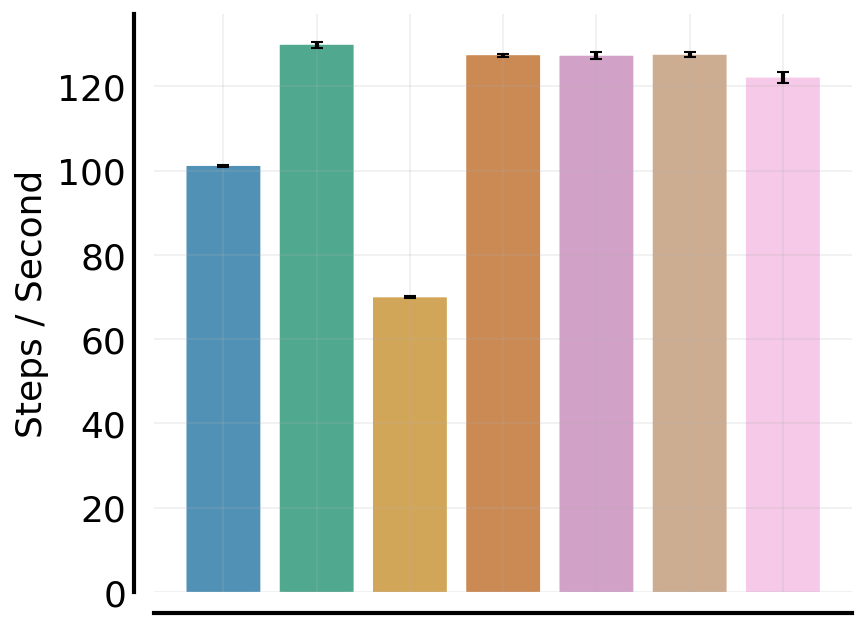
\includegraphics[width=0.31\linewidth]{figures/darkroom/inf_times/20x20.png}
        \label{fig:sub2}
    }
    \hfill
    \subfigure[Dark-Room 40$\times$20]{
        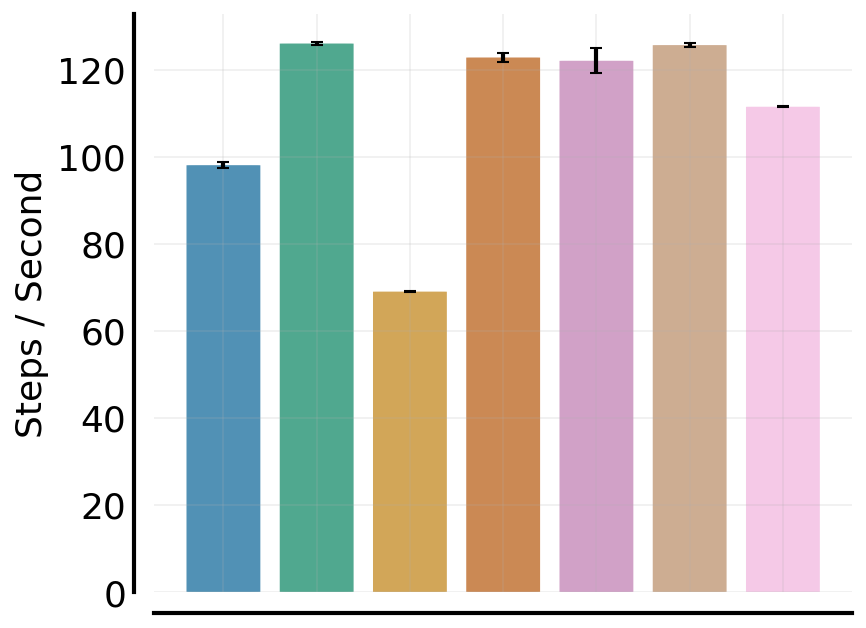
\includegraphics[width=0.33\linewidth]{figures/darkroom/inf_times/40x20.png}
        \label{fig:sub3}
    }
    \caption{Inference efficiency for all considered methods on \textbf{(a) Dark-Room 10$\times$10}, \textbf{(b) Dark-Room 20$\times$20}, \textbf{(c) Dark-Room 40$\times$20}. We measure inference efficiency in terms of the number of environment interaction steps performed per second (higher is better).}
    \label{fig:darkroom-inference-efficiency}
\end{figure*}

Note that the inference speed is roughly the same across grid sizes and consequently episode lengths. 
This suggests that the inference time is not yet dominated by the quadratic cost of self-attention for $B=1$ and the sequence lengths we consider in this analysis. 
This is because inference remains memory-bound with $B=1$ when using FlashAttention on the hardware setup we consider.
For environments with even longer episode lengths, higher batch sizes, or bigger models, the inference would move towards a compute-bound regime, and similar speed-ups for RA-DT are to be expected as for training time.
To further support this, we run an ablation in which we compare the inference efficiency for all baselines with and without FlashAttention (see Figure \ref{fig:ad-effect-of-fa}) on Dark-Room $40 \times 20$. 
Indeed, we observe a significant drop in inference speed when FlashAttention is disabled.  

\begin{figure}[h]
     \centering
     
\includegraphics[width=0.75\textwidth]{figures/darkroom/inf_times/legend_nofa.png}

     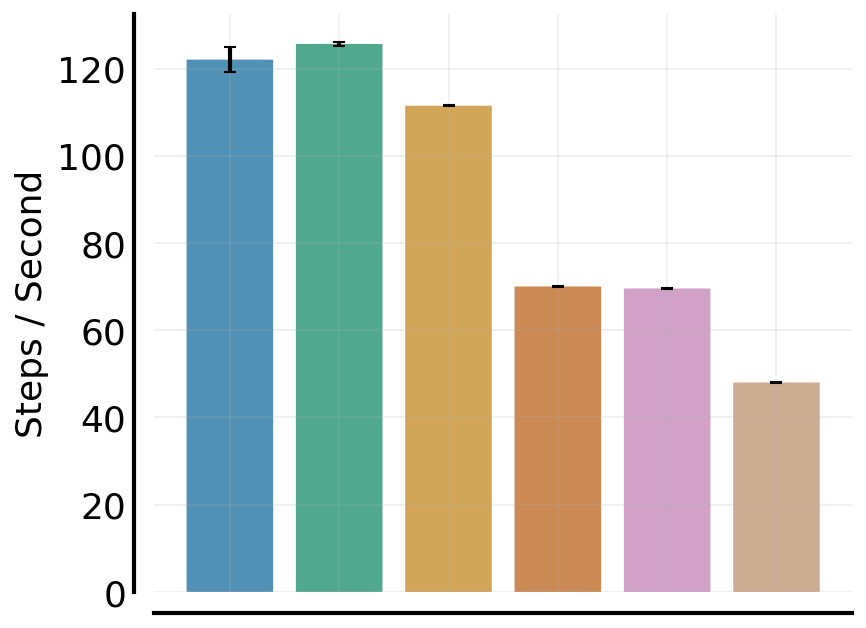
\includegraphics[width=0.31\textwidth]{figures/darkroom/inf_times/40x20_no_fa.png}
    \caption{Effect of FlashAttention on inference efficiency of AD, DPT, and DT on Dark-Room $40\times20$. Disabling FlashAttention results in a considerable drop in inference speed.}
    \label{fig:ad-effect-of-fa}
\end{figure}

\rebuttal{
To conclude this analysis, our findings indicate that while RA-DT is slightly slower when retrieving on every step, it achieves comparable inference speeds to the baselines when retrieving less frequently. 
Importantly, the retrieval mechanism in RA-DT enables access to the entirety of the experiences collected across all ICL trials.
In contrast, the baselines can only access experiences from a limited set of the most recent episodes that are preserved in the context (2 in our experiments). 
If we were to provide more context episodes to the baselines, the quadratic complexity of self-attention would kick in (similar to Figure \ref{fig:darkroom-training-efficiency}).
The ability of RA-DT to access a much broader set of experiences may be a reason for its enhanced downstream performance. 
}

\subsection{Pre-trained Language Model}
We investigate how strongly the ICL performance of RA-DT is influenced by the pre-trained LM used in our domain-agnostic embedding model.  
In Figure \ref{fig:ablation-lm}, we compare our default choice BERT \citep{Devlin:18} against four alternative encoder and decoder backbones, namely RoBERTa \citep{Liu:19}, DistilRoBERTa, DistilBERT \citep{Sanh:19}, and DistilGPT2. 
We find that RA-DT maintains decent performance across all pre-trained LMs, indicating robust retrieval performance across different LMs. 
Generally, the non-distilled variants outperform their distilled counterparts. 
Moreover, this experiment suggests a clear advantage of encoder-only models over the decoder-only LM, DistilGPT2. 
This suggests that the encoder-only LMs are better able to capture the relations between tokens within the token sequence, which leads to more precise retrieval of sub-trajectories and higher downstream performance.
\begin{figure*}[h]
    \centering
    
\includegraphics[width=0.85\linewidth]{figures/ablations/pretrained_lm/legend.png}
    
    \subfigure[80 Train Goals]{
        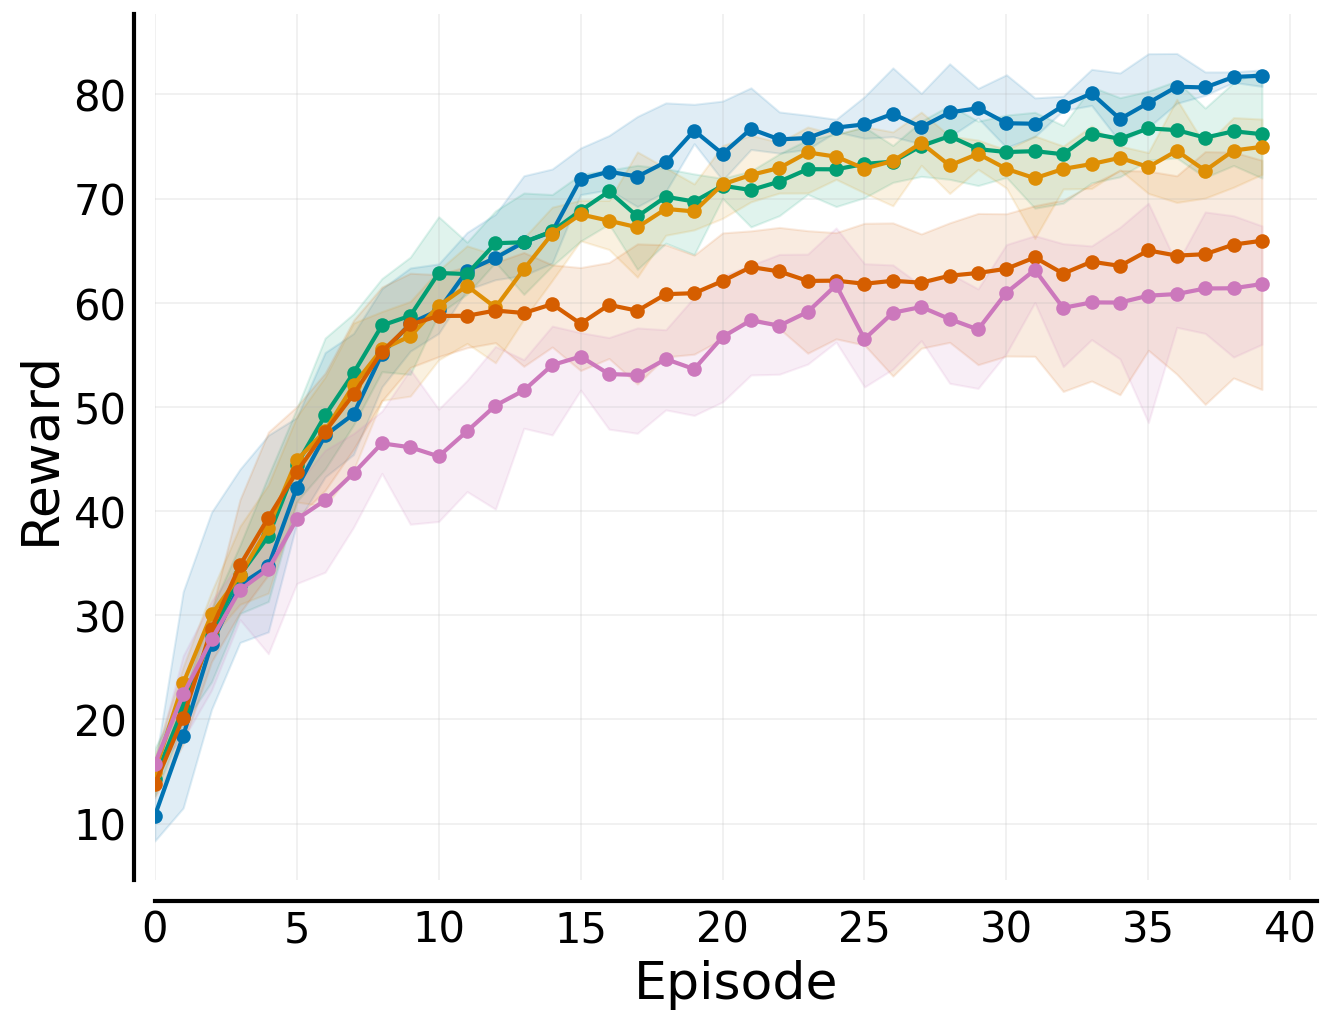
\includegraphics[width=0.31\linewidth]{figures/ablations/pretrained_lm/train_icl.png}
        \label{fig:sub1}
    }
    \hspace{1cm}
    \subfigure[20 Eval Goals]{
        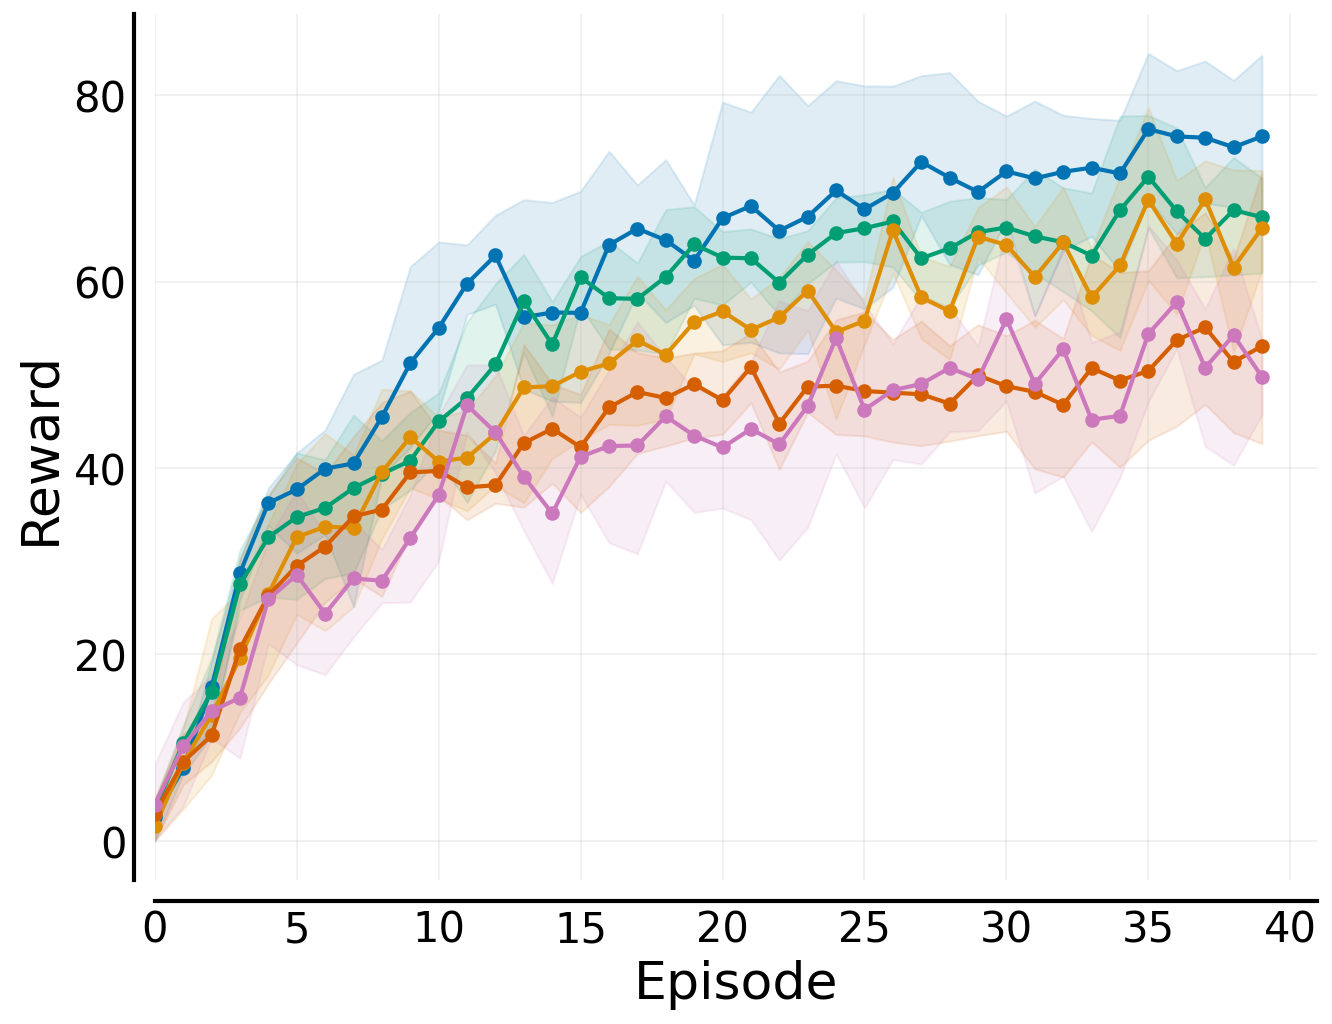
\includegraphics[width=0.31\linewidth]{figures/ablations/pretrained_lm/eval_icl.png}
        \label{fig:sub2}
    }
    \caption{Effect of the \textbf{Pre-trained LM}. Average performances on Dark-Room 10$\times$10 over the course of training for \textbf{(a)} train and \textbf{(b)} test tasks.}    
    \label{fig:ablation-lm}
\end{figure*}


\subsection{Effect of $K$ on Algorithm Distillation} \label{appendix:k-in-ad}
Finally, we investigate the effect of $K$ on the performance of AD. 
$K$ determines the number of episodes that have passed between the current and the context trajectory, which are provided to AD as the context. 
Consequently, $K$ specifies the extent of improvement observed between subsequent episodes.
By default, we use $K=100$ for our experiments on Dark-Room $10\times10$. 
Therefore, we conduct an ablation study, in which we vary $K$ (see Figure \ref{fig:ad-effect-of-k}.
We find that too small values for $K$ (e.g., 1 and 10) result in slow ICL behavior. 
In contrast, too high values for $K$ (e.g., 500) lead to fast initial progress but suboptimal performance in the long term. 
Only $K=100$ leads to steady improvement across all interaction episodes.
Consequently, AD requires careful tuning of $K$.

\begin{figure}[h]
     \centering
     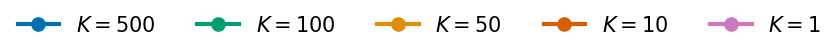
\includegraphics[width=0.6\textwidth]{figures/ablations/ad_k/legend.png}

     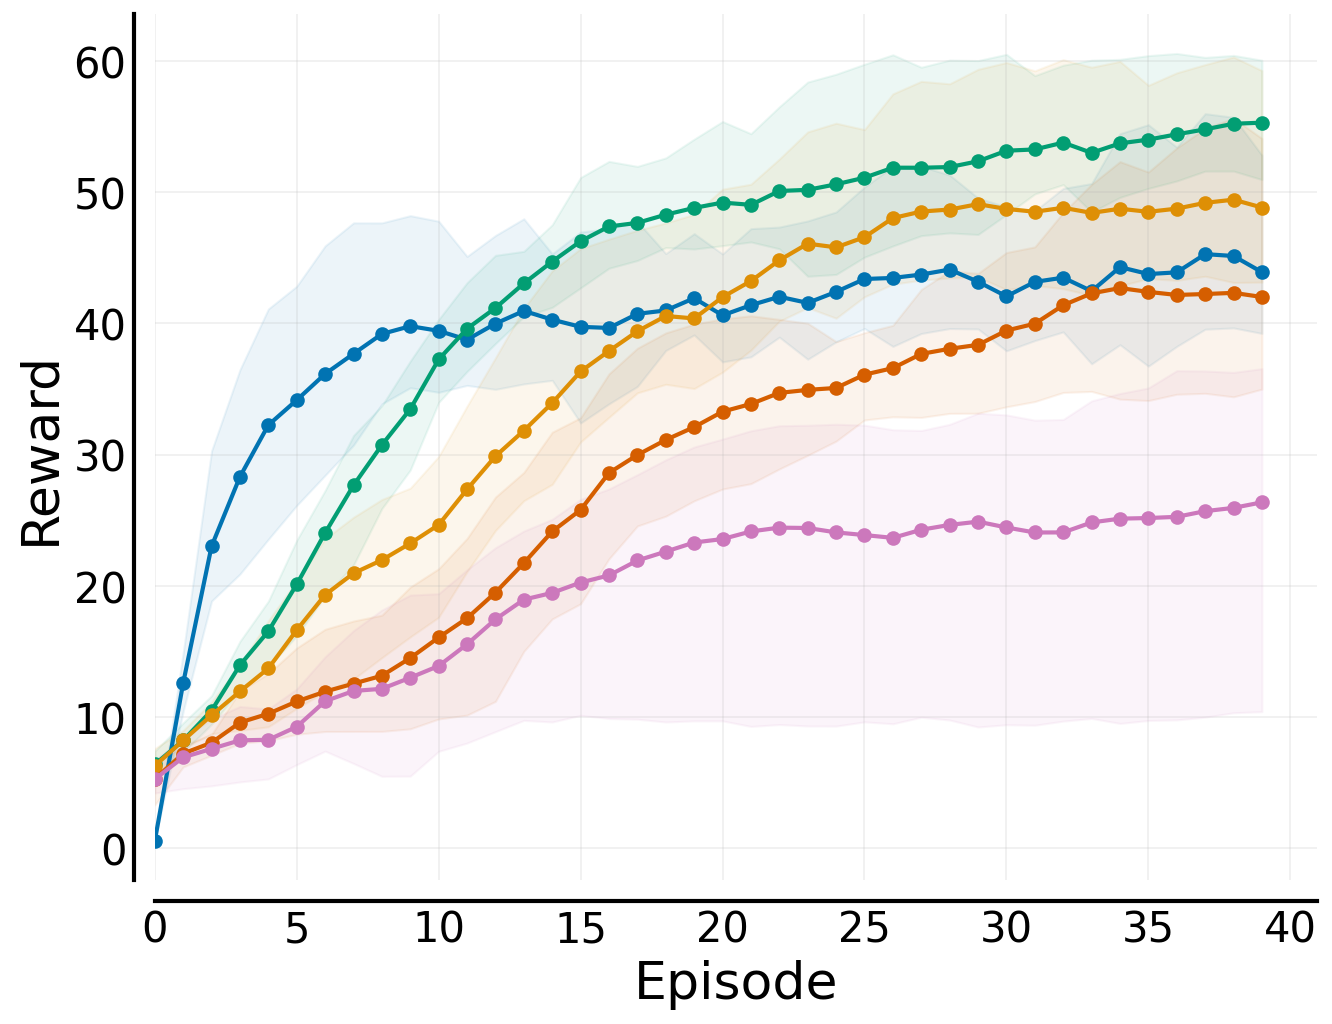
\includegraphics[width=0.31\textwidth]{figures/ablations/ad_k/darkroom10x10.png}
    \caption{Ablation on the number of episodes $K$ in AD that have passed between “current” trajectory and “context” trajectory on Dark-Room 10$\times$10. $K$ determines how much improvement is observed between episodes. We find that performance increases as $K$ increases, but only up to a certain point ($K=100$). With $K=500$, AD improves rapidly in the first few episodes, but then flattens out.}
    \label{fig:ad-effect-of-k}
\end{figure}

\subsection{Convergence of Baselines}
\rebuttal{
In the main experiments on grid-worlds reported in Section \ref{sec:exp-darkroom}, we found that the baselines AD and DPT only reach sub-optimal performance within the 40 ICL trials. 
Therefore, we analyse their performance when evaluating for more ICL trials.
In Figure \ref{fig:baselines-convergence}, we compare the evaluation performance of AD and DPT across 200 ICL trials on the 20 hold-out tasks for Dark-Room $10\times10$. 
We find that both methods continue to improve towards optimal performance in this environment when given more ICL trials.
For this ablation, we found it useful to set $K=50$ in AD (see Appendix \ref{appendix:k-in-ad}) instead of $K=100$ as used in our main experiments over 40 ICL trials.  
}

\begin{figure}[h]
     \centering
     
\includegraphics[width=0.2\textwidth]{figures/darkroom/converging_baselines/legend.png}

     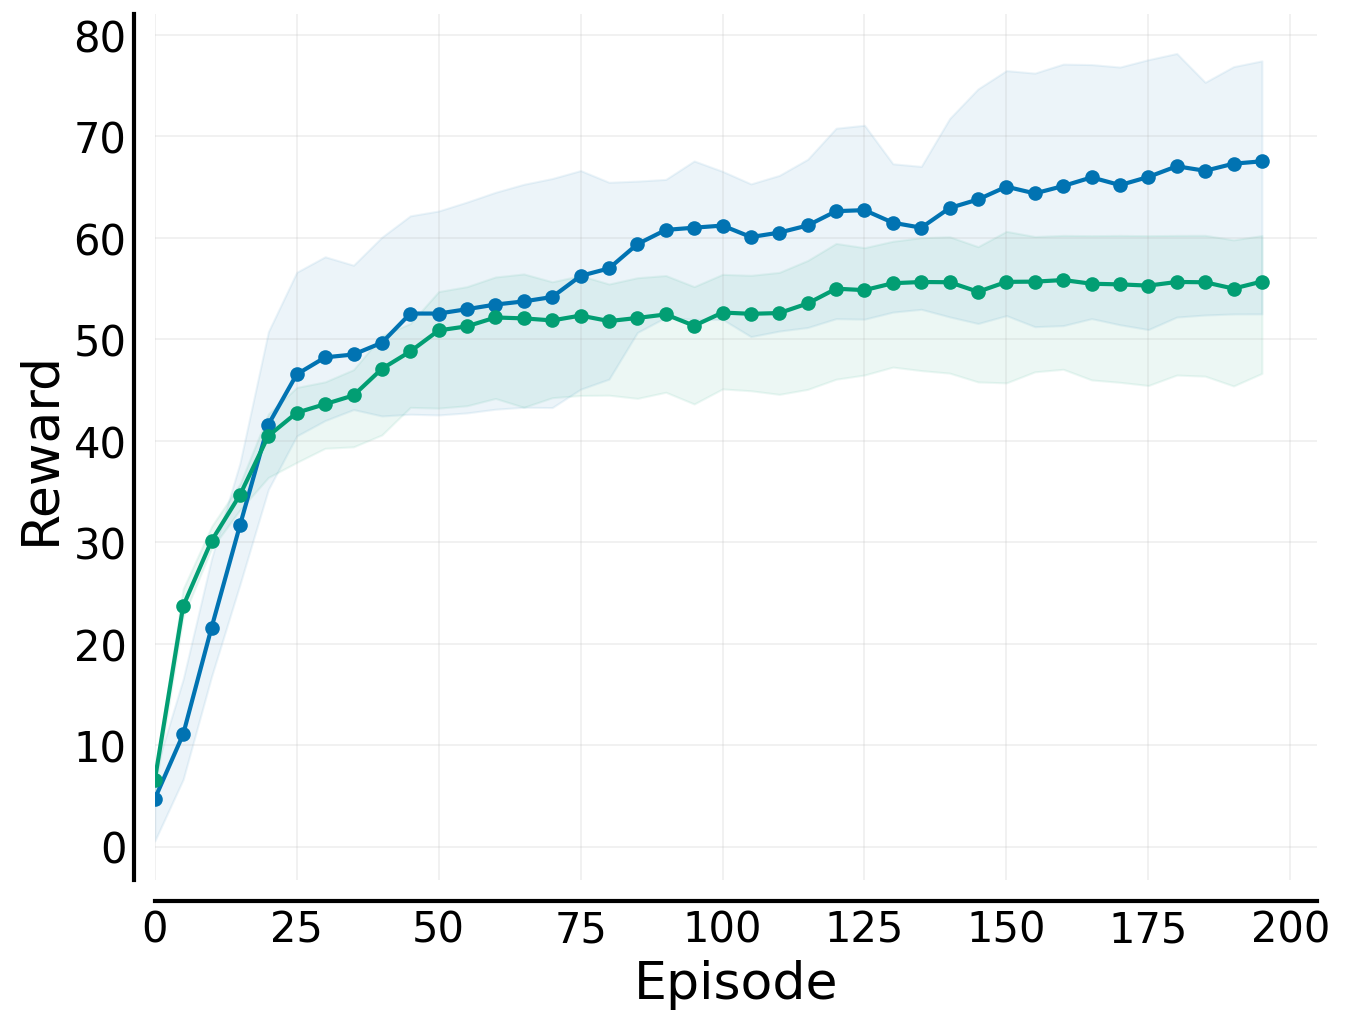
\includegraphics[width=0.31\textwidth]{figures/darkroom/converging_baselines/10x10.png}
    \caption{Evaluation of AD and DPT on Dark-Room 10$\times$10 over 200 ICL trials. Both methods continue to improve towards optimal performance in this environment.}
    \label{fig:baselines-convergence}
\end{figure}



